% \documentclass[draft]{beamer}
\documentclass{beamer}
\usepackage[latin1]{inputenc}
\usepackage{textpos}

\usepackage{graphics}
% \usepackage[demo]{graphicx}
\usepackage{adjustbox}

\usepackage[english]{babel}
\usepackage{colortbl}
\usepackage{caption}
% \usepackage{subcaption}
\usepackage{multirow}
\usepackage{amsmath}
\usepackage[makeroom]{cancel}
\usepackage{xcolor} % for colored text

\usepackage{tikz} % for flow charts
\usetikzlibrary{shapes,arrows,positioning,shadows,calc}

\usepackage{filecontents}% http://ctan.org/pkg/filecontents
\usepackage{silence}% http://ctan.org/pkg/silence
\WarningFilter{latex}{Overwriting file}% Remove LaTeX warnings starting with "Overwriting file"
\begin{filecontents*}{linereg.data}
#x y
0 4
10 24
\end{filecontents*} 

\begin{filecontents*}{linereg2.data}
#x y
2 8
8 20
\end{filecontents*} 

	\renewcommand<>{\item}[1]{\only#2{\beameroriginal{\item}{#1}}} % for replace a equation for other equation in the same place
	
	% \usetheme{Warsaw}
	\usetheme{Frankfurt}
	% \usetheme{Boadilla}
	\setbeamertemplate{navigation symbols}{} 
	% \useoutertheme{infolines} 
% \setbeamertemplate{footline}{\hbox{\vspace{0.1cm} \insertshortauthor \hspace*{3.5cm} \insertshorttitle \hspace*{4.0cm} \hfill\insertframenumber/\inserttotalframenumber}} 

\setbeamertemplate{footline}{\hbox{\vspace{0.1cm} \insertshortauthor \hspace*{3.5cm} \insertshorttitle \hspace*{4.4cm} \hfill\insertframenumber}} 

\def\braces#1{[#1]} % to define square parenthesis 
	
% \usecolortheme{orchid}

% \usecolortheme{lily}

% \usecolortheme{default}
\usecolortheme{cranejavier}

% \setbeamertemplate{footline}[frame number]
% \setbeamertemplate{footline}[page number]
	
	
	% -------------------------------------- Slide 1
	\title[Field Measurements and Instrumentation]{Intro to Instrumentation and Field Measurements in Remote Sensing}
	\author[J. Concha \& P. Romanczyk]{\Large Javier Concha and Paul Romanczyk}
	\institute{\footnotesize Digital Imaging and Remote Sensing Lab\\Chester F. Carlson Center for Imaging Science\\ Rochester Institute of Technology}
	\date{\today}


\AtBeginSection[ ]
{	\setbeamertemplate{footline}{} 	
	\begin{frame}{\LARGE Outline} 
	\LARGE
		\tableofcontents[currentsection]
	\end{frame}

\addtocounter{framenumber}{-1}	

\setbeamertemplate{footline}{\hbox{\vspace{0.1cm} \insertshortauthor \hspace*{2.0cm} \insertshorttitle \hspace*{3.8cm} \hfill\insertframenumber}} 
}	

% \AtBeginSubsection[ ]
% {		
% 	\begin{frame}{\LARGE Outline} 
% 		\tableofcontents[currentsection,currentsubsection]
% 	\end{frame}
% \addtocounter{framenumber}{-1}	
% }		
\newcounter{tmpc} % for resume counter
%&&&&&&&&&&&&&&&&&&&&&&&&&&&&&&&&&&&&&&&&&&&&&&&&&&&&&&&&&&&&&&&
%&&&&&&&&&&&&&&&&&&&&&&&&&&&&&&&&&&&&&&&&&&&&&&&&&&&&&&&&&&&&&&&
\begin{document}
{	
\setbeamertemplate{footline}{} 
\setbeamertemplate{headline}{}
	
	\begin{frame} 
	\titlepage
	
	\begin{textblock*}{10cm}(10.0cm,-8.2cm)
	   
\includegraphics[height=10mm]{Images/tiger_walking_rit_color.eps}
	\end{textblock*}
	
	\begin{textblock*}{10cm}(-.7cm,-8.2cm)
	   
\includegraphics[height=10mm]{./Images/dirs_logo.png}
	\end{textblock*}
	
	\begin{textblock*}{9cm}(2cm,-4.5cm)

	   \tikz\node[opacity=0.3]{ 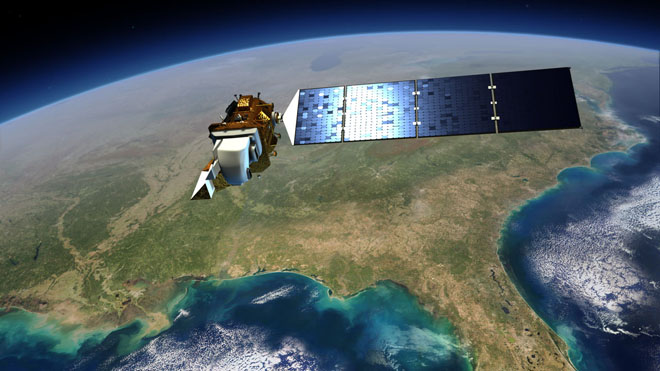
\includegraphics[width=65mm]{./Images/landsat8-earth.jpg}};
	\end{textblock*}

	\begin{textblock*}{12cm}(3.0cm,0cm)
	   \scriptsize Presented for 2015 Intersession Term
	\end{textblock*}
	
	\end{frame}

}
\addtocounter{framenumber}{-1}
%\setbeamercovered{highly dynamic}
%\setbeamercovered{transparent}
\setbeamercovered{still covered={\opaqueness<1->{2}},again covered={\opaqueness<1->{2}}}

% ----------------------------------- Slide ----------------------------------------------	

\addtobeamertemplate{frametitle}{}{%
\begin{textblock*}{90mm}(8.2cm,-0.5cm)
% \includegraphics[height=0.5cm]{/Users/javier/Desktop/Javier/MASTER_RIT/SPIE2012/Slides/rit_white_no_bar.jpg}

\includegraphics[height=0.4cm]{./Images/RIT_LOGO.png}
\end{textblock*}}


% ----------------------------------- Slide ----------------------------------------------
{
\setbeamertemplate{footline}{} 
\begin{frame}{\LARGE Outline} 
\LARGE
	\tableofcontents
\end{frame}

\addtocounter{framenumber}{-1}
}

%%%%%%%%%%%%%%%%%%% SECTION %%%%%%%%%%%%%%%%%%%%%%%%%%%%%%%%
\section{Introduction}
\subsection*{Motivation}
% --- slide ------------------------------------------------
\begin{frame}{\LARGE Course Goals} 
\LARGE
\begin{itemize}\itemsep.4cm
	\item Learn the importance of field measurements
	\item Learn how to take field measurements
	\item Learn about DIRS instruments
\end{itemize}
\end{frame}
% --- slide ------------------------------------------------
\begin{frame}{\LARGE Course Description} 
\LARGE
\begin{itemize}\itemsep.4cm
	\item Friday: Introduction
	\item Monday: Introduction (con't) and DIRS instruments exhibition
	\item Tuesday: Lab: Reflectance measurements
	\item Wednesday: Lab: LIDAR measurements
\end{itemize}
\end{frame}
% --- slide ------------------------------------------------
\begin{frame}{\LARGE Definitions} 
\Large

\begin{itemize}\itemsep.5cm
	\item {\bf Remote Sensing:}\\
``Remote sensing is the science of obtaining information about objects or areas from a distance, typically from aircraft or satellites.''\\
	\item {\bf Field Measurements or Groundtruth or Ground-based data or reference data or ancillary data:}\\

``Observations or measurements made at or near the surface of the earth in support of remote sensing.''\\

\end{itemize}

\end{frame}
% --- slide ------------------------------------------------
\begin{frame}{\LARGE Motivation}
\LARGE
{\bf Why is it important?}\\
\begin{itemize}\itemsep.3cm
	\item Validation: comparison to know how close a model is to the field measurements (accuracy)
	\item Calibration or Correction: adjust model or instrument to be more precise (data fitting)
	\item Data collection to get characteristics of target, materials, etc.
\end{itemize}
\end{frame}
% % --- slide ------------------------------------------------
% \begin{frame}{\LARGE Motivation}{\vspace{0.1cm} \Large Examples}
% \vspace{-.7cm}
% Include:\\
% Javier's example (over water mea.)\\
% Paul's example (LIDAR and trees?)

% \end{frame}
% --- slide ------------------------------------------------
\begin{frame}{\LARGE Example: Field Data Collection }{\vspace{0.1cm} \Large Area of Study}
\begin{figure}[htb]
  \centering
	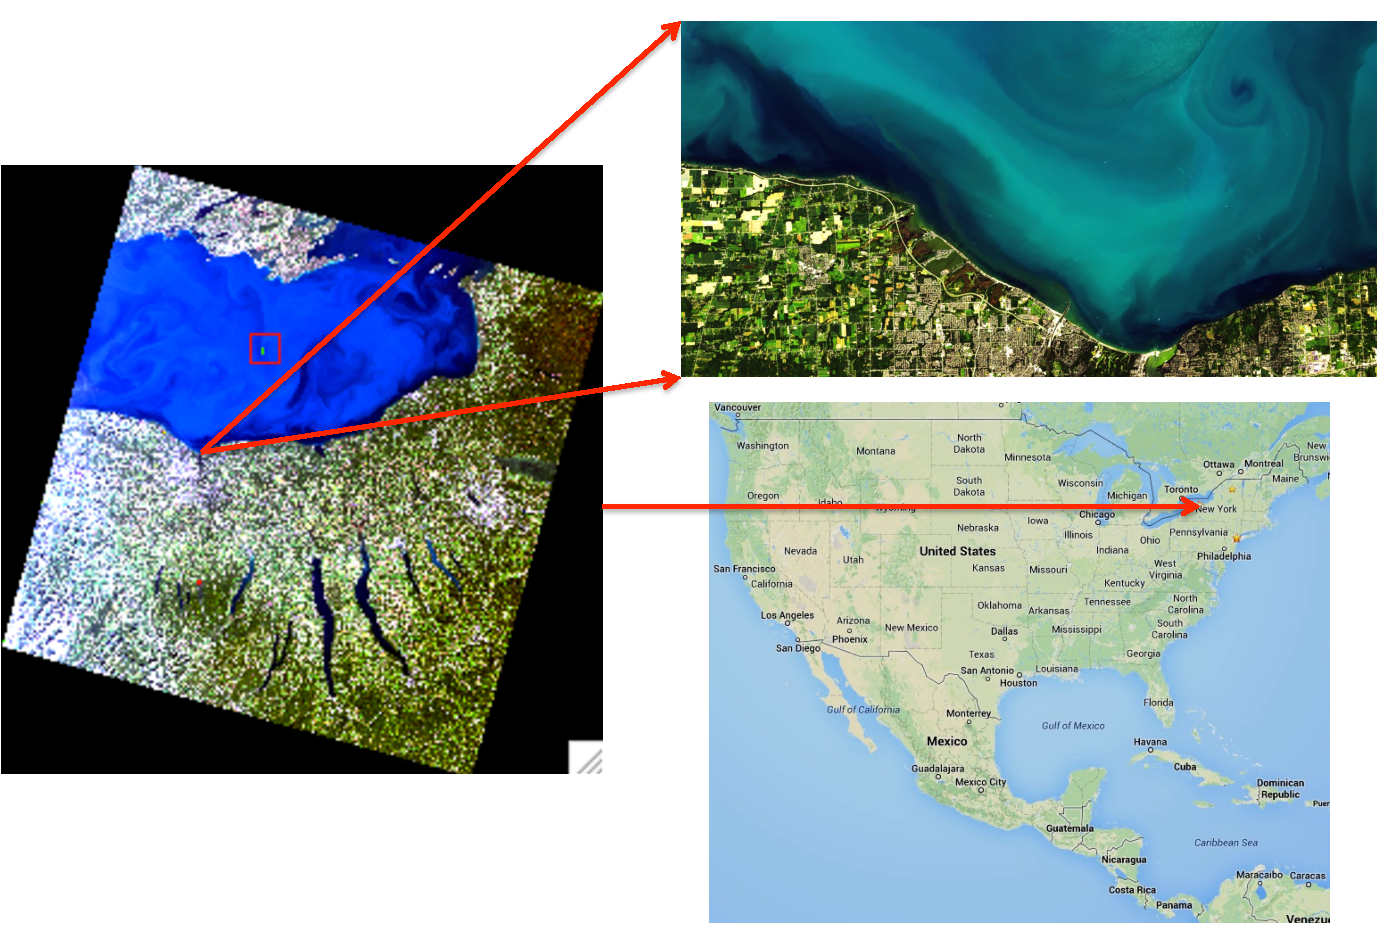
\includegraphics[height=7cm]{./Images/AreaOfStudy1.pdf} 
  % \caption{Sites in the Rochester Embayment for the water sample collection on September, $19^{th}$, 2013.\label{fig:0910913Sites} } 
\end{figure}
\end{frame}
% --- slide ------------------------------------------------
\begin{frame}{\LARGE Field Data Collection (con't)}{\vspace{0.1cm} \Large Area of Study}
\begin{figure}[htb]
  	\centering
  	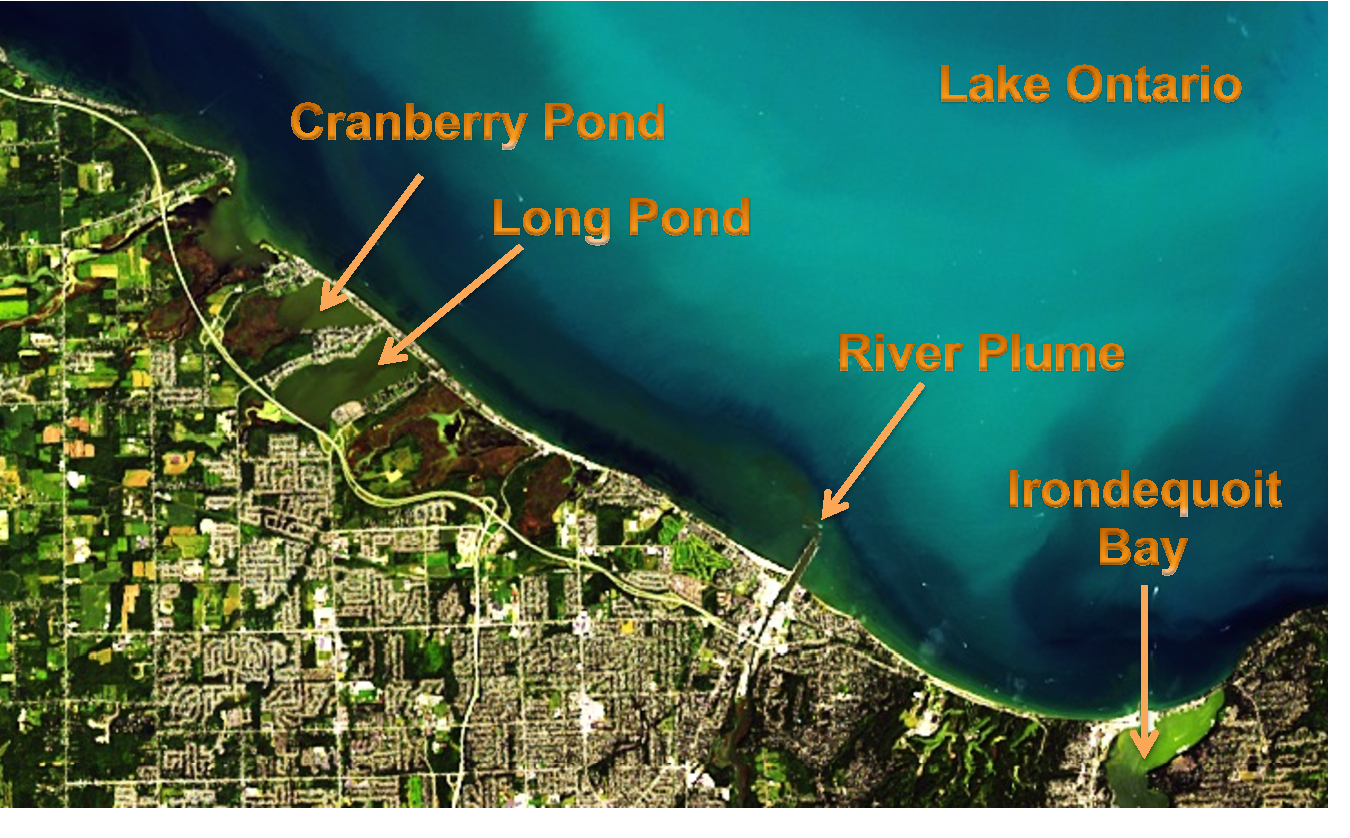
\includegraphics[height=6cm]{./Images/AreaOfStudy2.pdf}
\end{figure}
\end{frame}
% --- slide ------------------------------------------------
\begin{frame}{\LARGE Field Data Collection (con't)}
\vspace{-1cm}
\begin{figure}[htb]
\centering
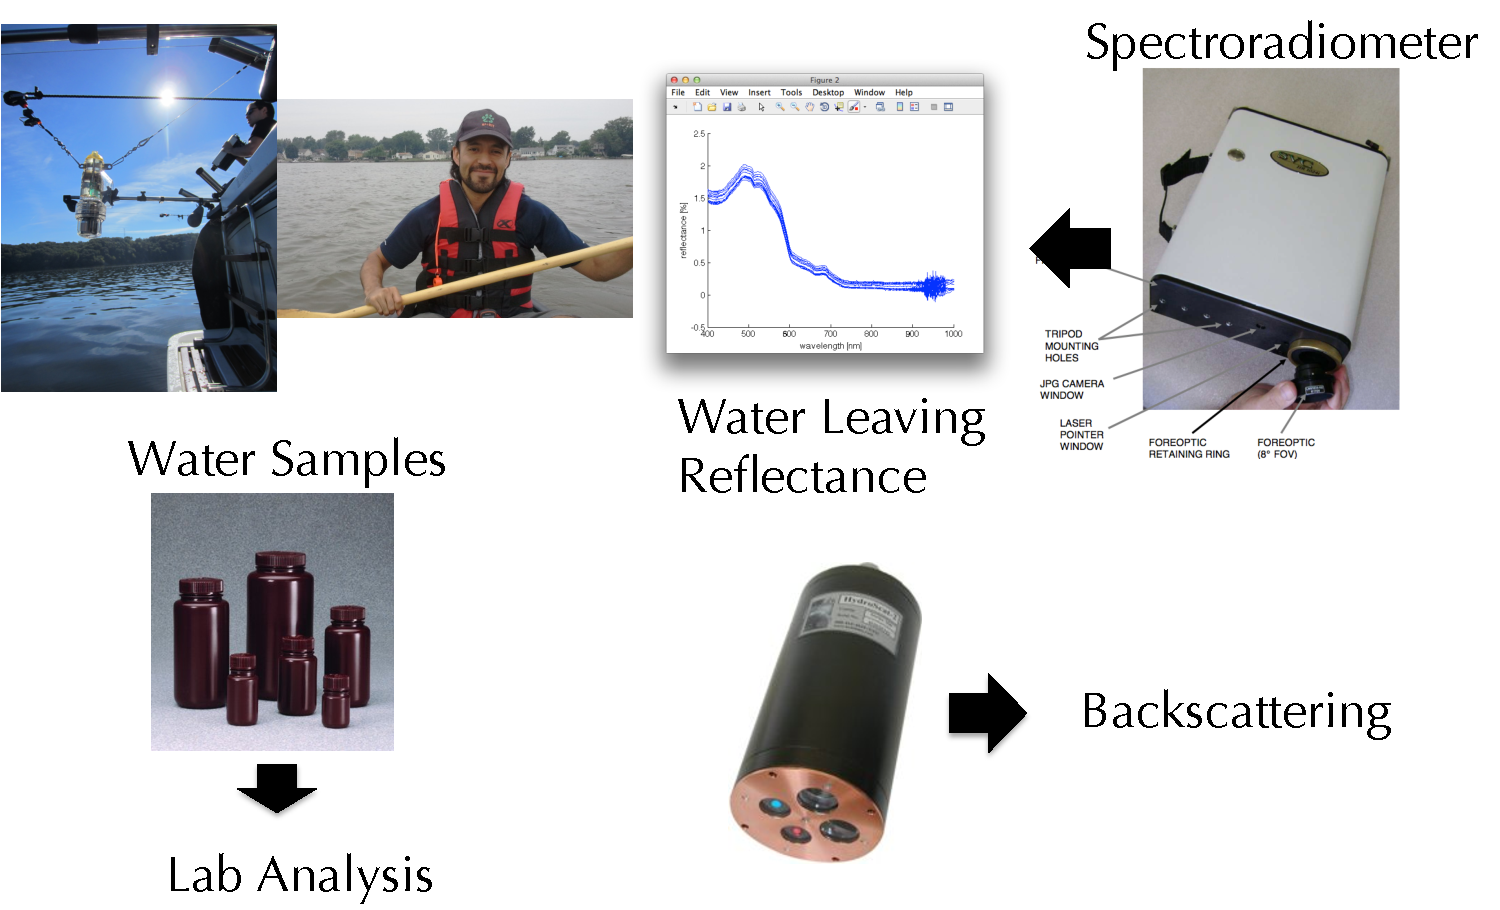
\includegraphics[height=7cm]{./Images/Collection.pdf}
      
\end{figure}
% \centerline{Comparison between traditional ELM (dashed lines)}
% \centerline{and model-based ELM (solid lines).}
\end{frame}
% --- slide ------------------------------------------------
\begin{frame}{\LARGE Field Data Collection (con't)}{\Large Lab Measurements} 
\vspace{-1cm}
\begin{figure}[htb]
\centering
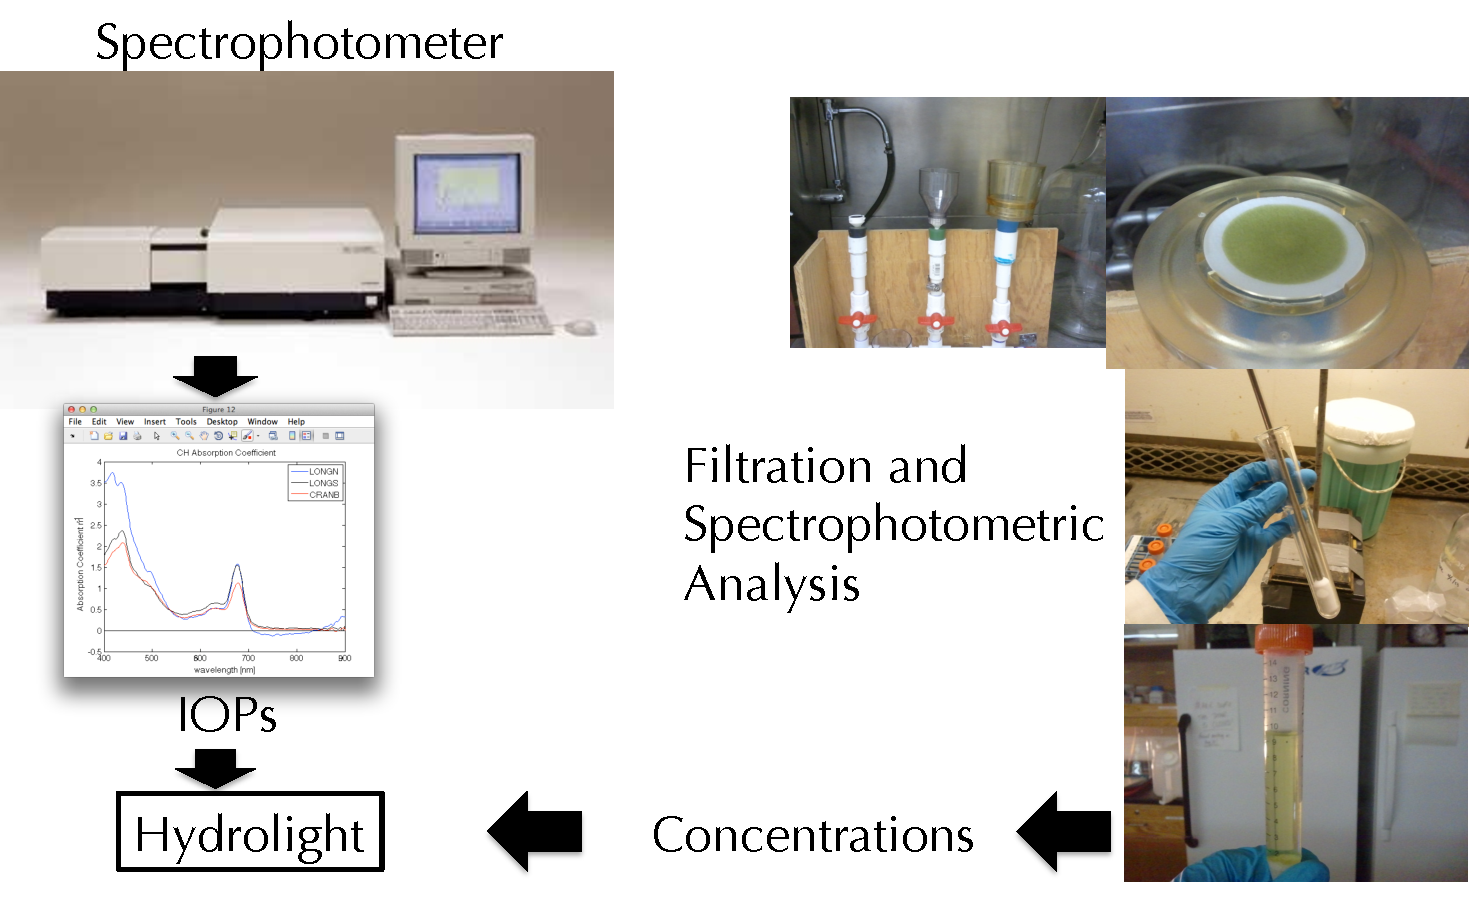
\includegraphics[height=7cm]{./Images/LabMeasurements.pdf}
      
\end{figure}
% \centerline{Comparison between traditional ELM (dashed lines)}
% \centerline{and model-based ELM (solid lines).}
\end{frame}
% --- slide ------------------------------------------------
\begin{frame}{\LARGE Field Data Collection (con't)}{\vspace{0.1cm} \Large 2013 and 2014 Seasons}
\begin{table}[htb]
  
  \centering
  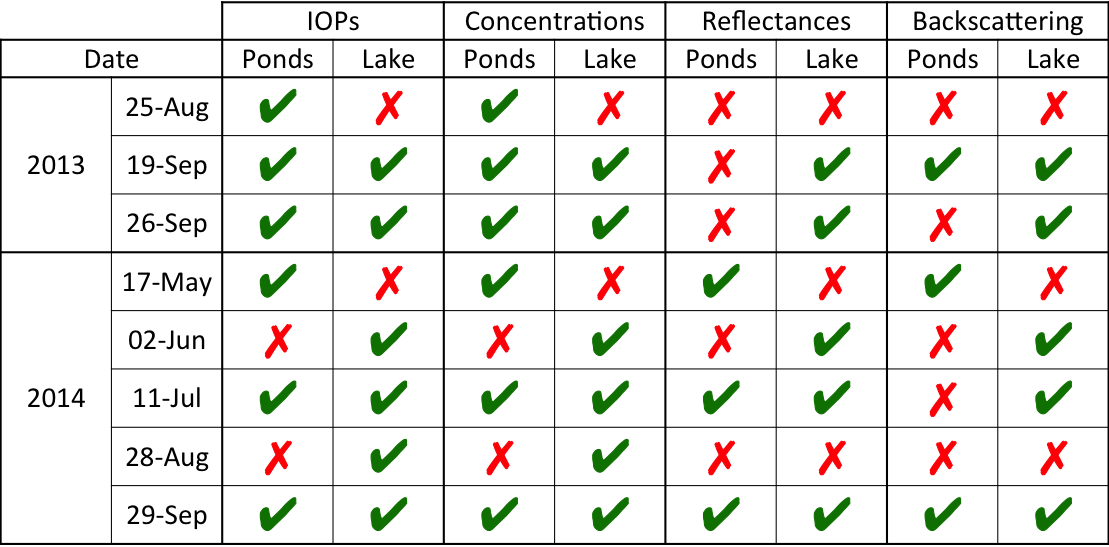
\includegraphics[width=11cm]{./Images/Collect1314.png}
  \label{tab:collect}
\end{table}
\end{frame}
% --- slide ------------------------------------------------
\begin{frame}{\LARGE Retrieval}{\vspace{.1cm} \Large Concentration Maps}
% \vspace{-.3cm}
\centering
\begin{figure}[htb]
\centering
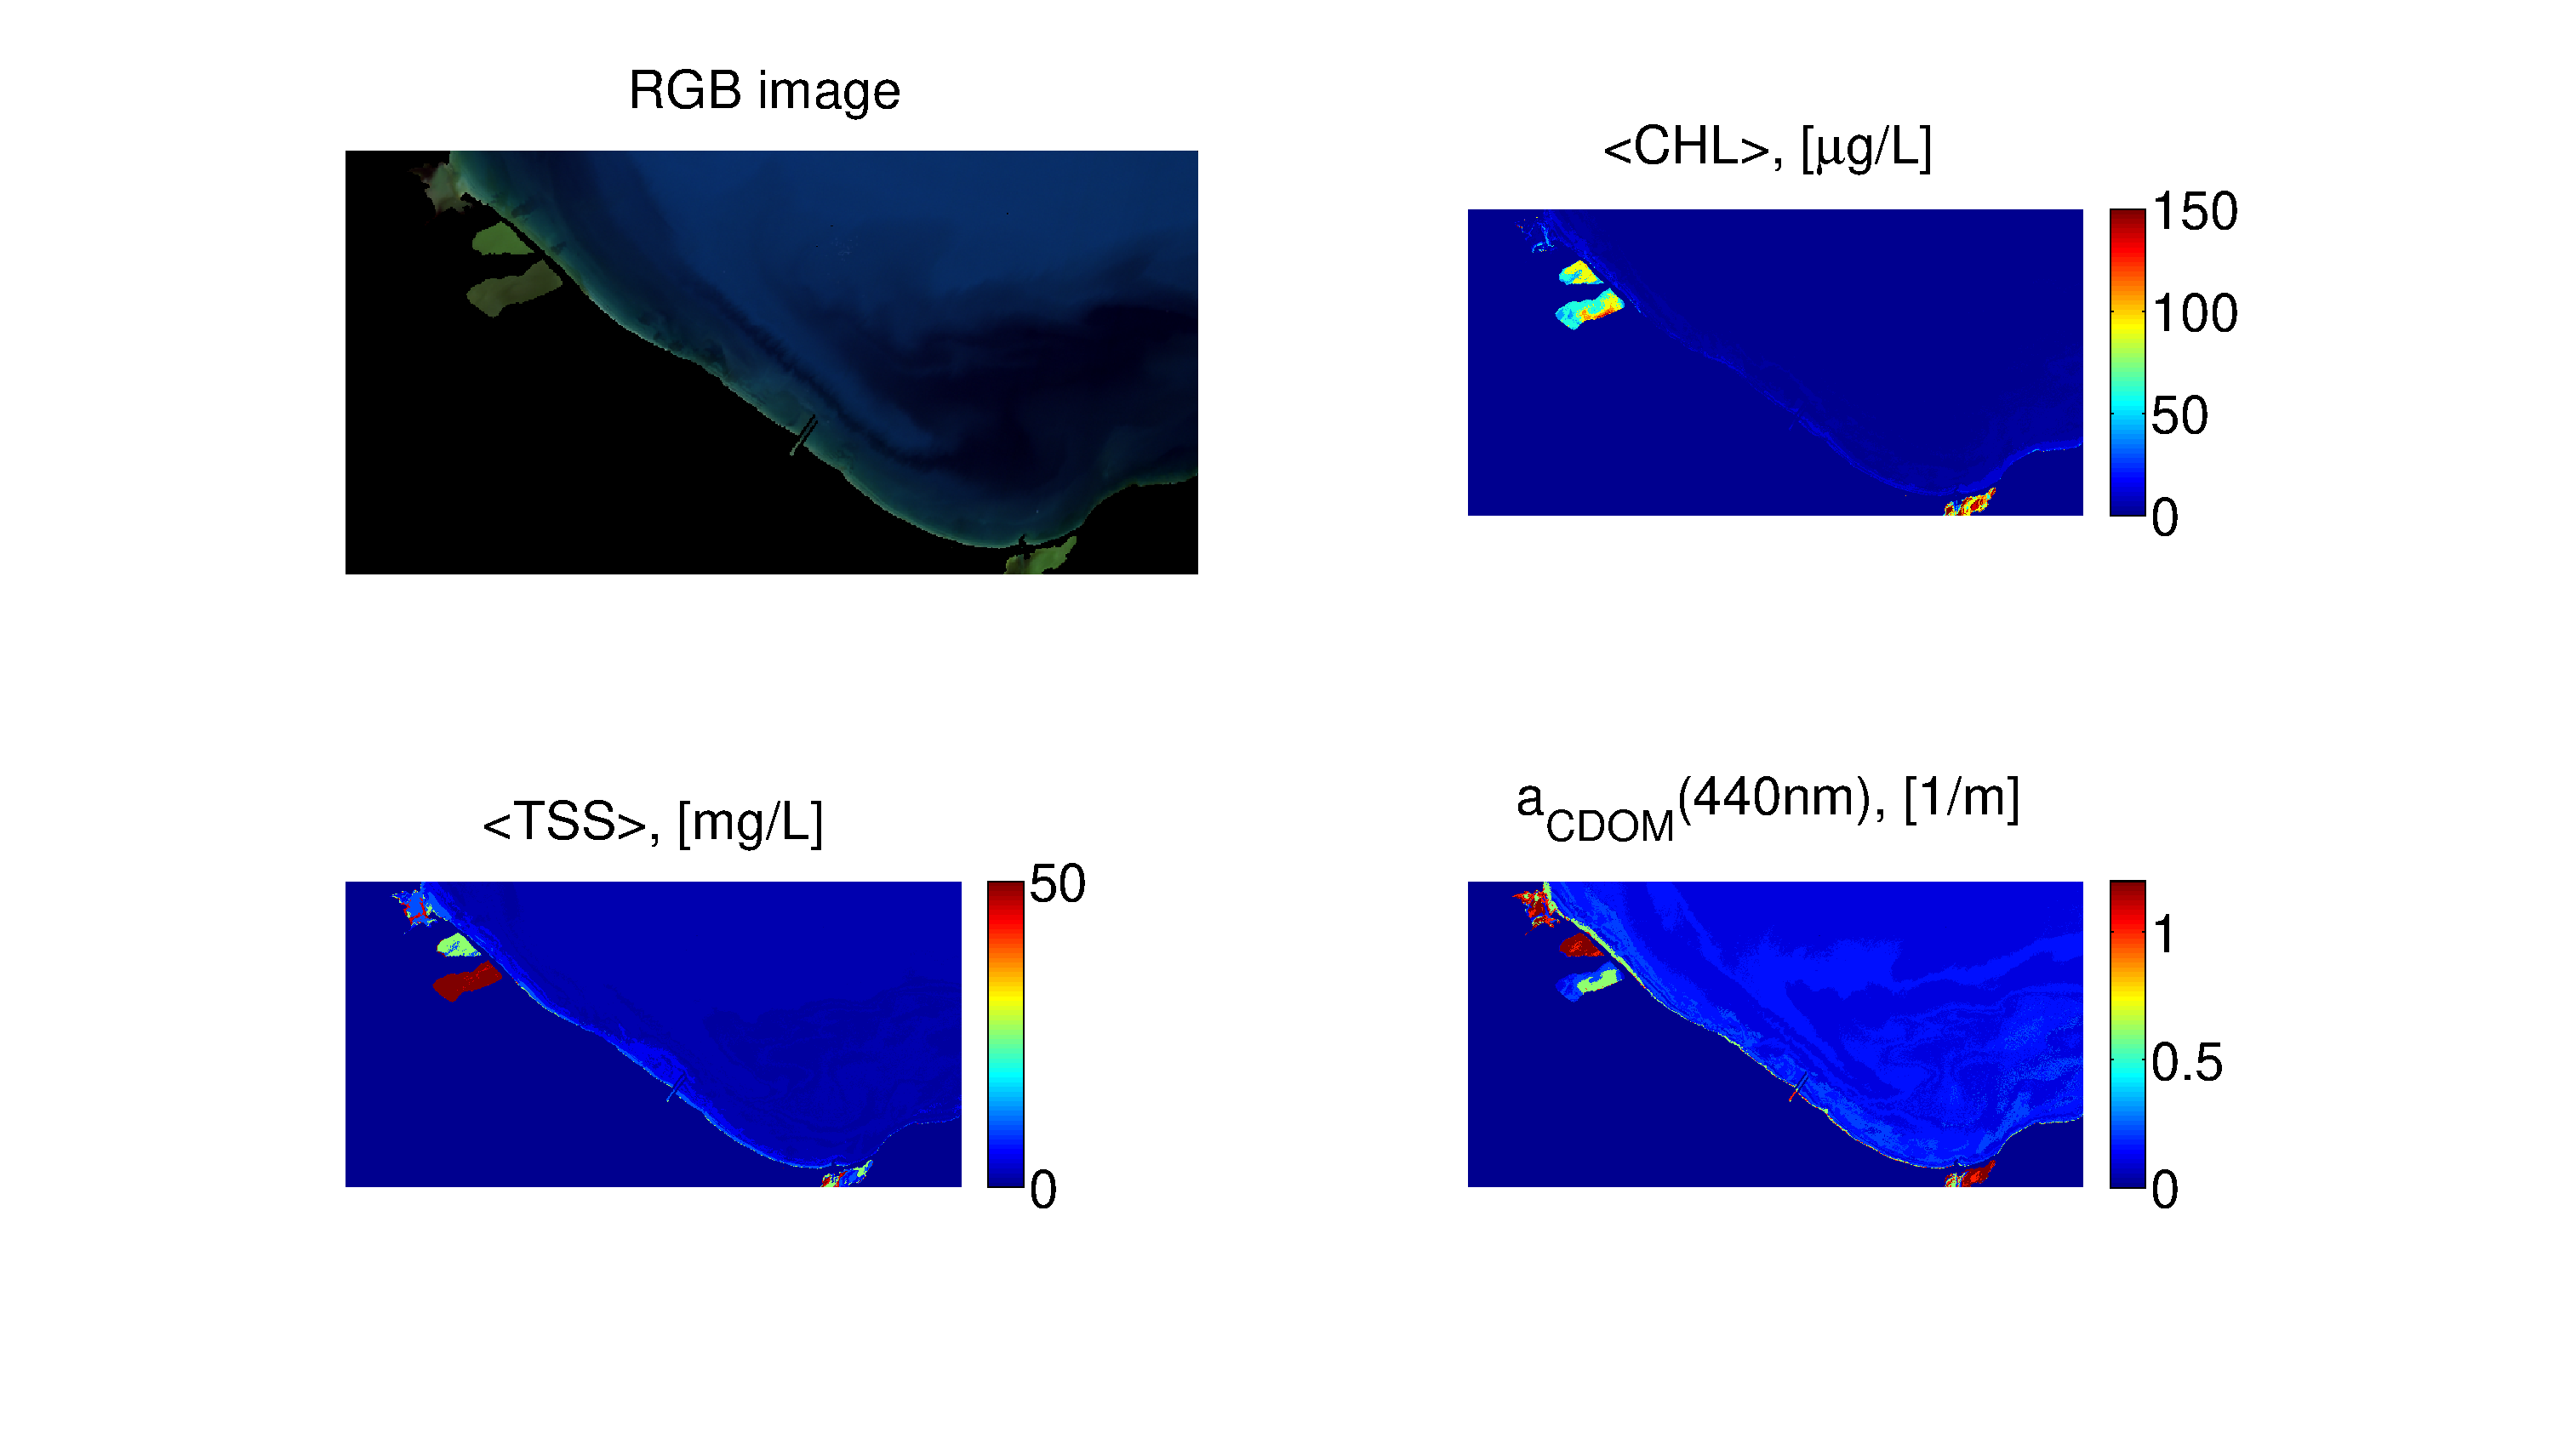
\includegraphics[trim=200 0 180 0,clip,height=8cm]{./Images/RetrievalResults.eps}
      
\end{figure}
% \centerline{Comparison between traditional ELM (dashed lines)}
% \centerline{and model-based ELM (solid lines).}
\end{frame}
% --- slide ------------------------------------------------
\begin{frame}{\LARGE Field Data Use}
\Large
\begin{itemize}\itemsep.5cm
	\item Reflectance: Atmospheric Correction
	\item Chl-{\it a} concentration: comparison with model
\end{itemize}

\end{frame}
%%%%%%%%%%%%%%%%%%% SECTION %%%%%%%%%%%%%%%%%%%%%%%%%%%%%%%%
\section{Background}
\subsection*{}
% --- slide ------------------------------------------------
\begin{frame}{\LARGE Examples of Kind of Measurements} 
\Large
\begin{itemize}\itemsep.4cm
	\item Reflectance: Radiometer
	\item Concentration: Spectrophotometer
	\item Location: GPS
	\item Structure: LIDAR
	\item Leaf Area Index (LAI): Ceptometer
\end{itemize}

\end{frame}
% --- slide ------------------------------------------------
\begin{frame}{\LARGE Radiometric Quantities: Radiance} 
% \begin{frame}{Radiometric Quantities: Radiance}
\begin{figure}[H]
\begin{columns}[t] % contents are top vertically aligned
	\begin{column}[T]{6cm} % each column can also be its own environment
  		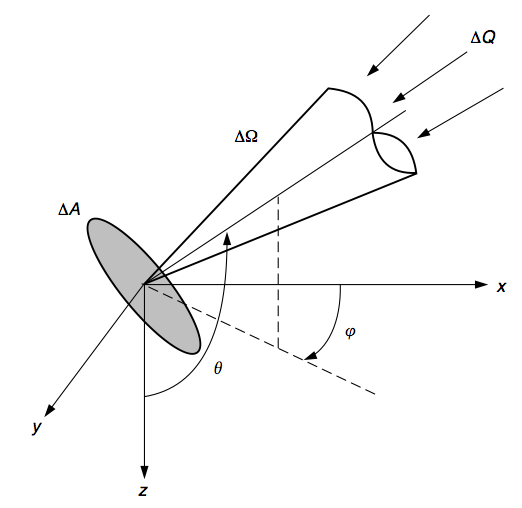
\includegraphics[height=6cm]{./Images/RadianceDef.png}
    \end{column}
	\begin{column}[T]{4cm} % each column can also be its own environment
  		$\Delta Q$: radian energy incident \\
  		$\Delta t$: time interval \\
  		$\Delta A$: surface area at location (x,y,z)\\
  		$\Delta\Omega$: solid angle in direction ($\theta$,$\varphi$) \\
  		$\Delta\lambda$: photons wavelength interval
    \end{column}
\end{columns}	
\end{figure}
\only<1>{\begin{equation}
	\small L(x,y,z,t,\theta,\varphi,\lambda)\equiv\frac{\Delta Q}{\Delta t\Delta A\Delta\Omega\Delta\lambda}~~\left[ Js^{-1}m^{-2}sr^{-1}nm^{-1} \right]
		\end{equation}}
\only<2>{\begin{equation}
	\small L(x,y,z,t,\theta,\varphi,\lambda)\equiv\frac{\partial^4 Q}{\partial t\partial A\partial\Omega\partial\lambda}~~\left[ Js^{-1}m^{-2}sr^{-1}nm^{-1} \right]
		\end{equation}}
\end{frame}
% --- slide ------------------------------------------------
\begin{frame}{\LARGE Radiance Sensor} 
\begin{figure}
\centering
    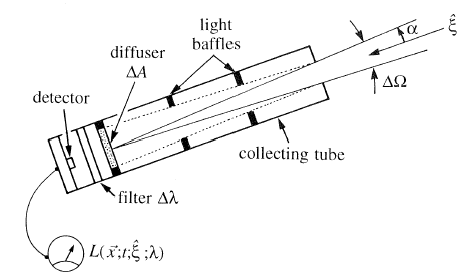
\includegraphics[height=5cm]{./Images/RadianceSensor.png}
\end{figure}
\vspace{-.7cm}
\hfill \scriptsize (Source: \cite{MobleyOnline})

% \vspace{0.2cm}
% \centerline{Water Pixels}
% \centerline{(Unknown concentrations)}

\end{frame}
% --- slide ------------------------------------------------
\begin{frame}{Radiometric Quantities: Irradiance}
\textbf{Spectral downwelling scalar irradiance} at depth z:
\begin{equation}
	E_{od}(z,\lambda)=\int_{2\pi_d} L(z,\theta,\varphi,\lambda)d\Omega~~\left[Wm^{-2}nm^{-1} \right]
\end{equation}
\textbf{Spectral upwelling scalar irradiance} at depth z:
\begin{equation}
	E_{ou}(z,\lambda)=\int_{2\pi_u} L(z,\theta,\varphi,\lambda)d\Omega~~\left[Wm^{-2}nm^{-1} \right]
\end{equation}
\textbf{Spectral scalar irradiance} at depth z:
\begin{align}
	E_{o}(z,\lambda) &\equiv E_{od}(z,\lambda)+E_{ou}(z,\lambda)\\
					 &=\int_{4\pi} L(z,\theta,\varphi,\lambda)d\Omega
\end{align}
\end{frame}
% --- slide ------------------------------------------------
\begin{frame}{\LARGE Scalar Irradiance Sensor} 
\begin{figure}
\centering
    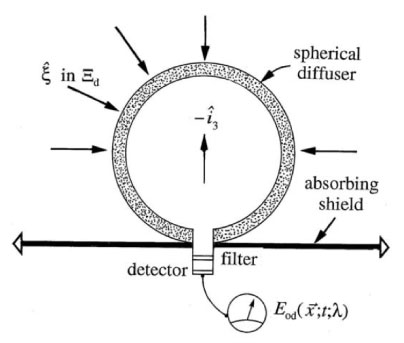
\includegraphics[height=5cm]{./Images/ScalarIrradianceSensor.jpg}
\end{figure}
\vspace{-.7cm}
\hfill \scriptsize (Source: \cite{MobleyOnline})

% \vspace{0.2cm}
% \centerline{Water Pixels}
% \centerline{(Unknown concentrations)}

\end{frame}
% --- slide ------------------------------------------------
\begin{frame}{Radiometric Quantities: Irradiance}
\textbf{Spectral downwelling plane irradiance} at depth z:
\begin{equation}
	E_{d}(z,\lambda)=\int_{2\pi_d} L(z,\theta,\varphi,\lambda)|cos\theta|d\Omega~~\left[Wm^{-2}nm^{-1} \right]
\end{equation}
Photosynthetic available radiation, \textbf{PAR}:
\begin{equation}
	PAR(z)\equiv \int_{350nm}^{700nm} \frac{\lambda}{hc}E_o(z,\lambda)d\lambda~~~\left[photons~s^{-1}m^{-2} \right]
\end{equation}
\end{frame}
% --- slide ------------------------------------------------
\begin{frame}{\LARGE Planar Irradiance Sensor} 
\begin{figure}
\centering
    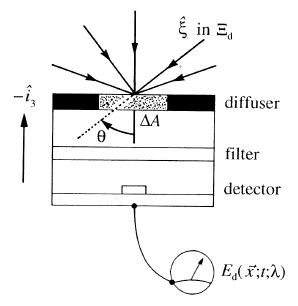
\includegraphics[height=5cm]{./Images/PlaneIrradianceSensor.png}
\end{figure}
\vspace{-.7cm}
\hfill \scriptsize (Source: \cite{MobleyOnline})

% \vspace{0.2cm}
% \centerline{Water Pixels}
% \centerline{(Unknown concentrations)}

\end{frame}
% --- slide ------------------------------------------------
\begin{frame}{Reflectance}
\begin{itemize}\itemsep.4cm
	\item {\textbf{Irradiance reflectance:}\\
			\begin{equation}
				R(z,\lambda)\equiv \frac{E_u(z,\lambda)}{E_d(z,\lambda)}
			\end{equation}}\\
	\item{ \textbf{Remote sensing reflectance (water):}\\
			\begin{equation}
				R_{rs}(\theta,\varphi,\lambda)\equiv \frac{L_w(\theta,\varphi,\lambda)}{E_d(\lambda)}~~\left[sr^{-1} \right]
			\end{equation}\\
			where $L_w$ is the \textbf{water-leaving radiance}\\}
	\item{ \textbf{Bidirectional Reflectance Distribution Function (BRDF):}\\
			\begin{equation}
				r_{BRDF} = \frac{\displaystyle L(\theta_o,\phi_o)}{\displaystyle E(\theta_i,\phi_i)}~~~\left[sr^{-1}\right]
			\end{equation}}
\end{itemize}
\end{frame}

%%%%%%%%%%%%%%%%%%% SECTION %%%%%%%%%%%%%%%%%%%%%%%%%%%%%%%%
\section{Preparation}
\subsection*{}
% --- slide ------------------------------------------------
\begin{frame}{Preparation}
	What do I want to collect?
	\begin{itemize}
		\item What instruments do I need?
		\item Where do I need to go?
		\item When do I need to go?
		\item How many people do I need?
	\end{itemize}
\end{frame}

% --- slide ------------------------------------------------
\begin{frame}{Preparation}
	Permits and forms
	\begin{itemize}
		\item RIT Risk management
		\scriptsize{\href{https://www.rit.edu/fa/grms/sites/rit.edu.fa.grms/files/docs/Agreement.pdf}{https://www.rit.edu/fa/grms/sites/rit.edu.fa.grms/files/docs/Agreement.pdf}}\normalsize
		\item Permits do do research
		\item RIT IRB
		\item Equipment checklist
		\item Data sheets
	\end{itemize}
\end{frame}

% --- slide ------------------------------------------------
\begin{frame}{Preparation}
	Safety
	\begin{itemize}
		\item Have a contact list (email, cell phone, other)
		\begin{itemize}
			\item Everyone in the field
			\item People back at RIT
			\item External contacts
			\item Emergency numbers 
		\end{itemize}
		\item First aid kit
		\item Water
		\item Food
	\end{itemize}
\end{frame}

% --- slide ------------------------------------------------
\begin{frame}{Preparation}
	Instruments
	\begin{itemize}
		\item Know how to use the instruments
		\item Make sure the batteries are charged
		\item Make sure there is room for new data
	\end{itemize}
\end{frame}

% --- slide ------------------------------------------------
\begin{frame}{Preparation}
	Other things to consider
	\begin{itemize}
		\item Shipping
		\item Driving
		\item How to get to the field
		\item Prioritization of data
		\item Ensure equipment availability
		\item Tools
		\item Write down procedure
		\item Sampling
		\item Take pictures
	\end{itemize}
\end{frame}

%%%%%%%%%%%%%%%%%%% SECTION %%%%%%%%%%%%%%%%%%%%%%%%%%%%%%%%
\section{Taking Measurements}
\subsection*{}
% --- slide ------------------------------------------------
\begin{frame}{Diffuse white reference panel (Spectralon)}
\begin{columns}[c] % contents are top vertically aligned
  	\begin{column}[T]{5cm}
  	\vspace{2cm}
		\begin{itemize}\itemsep.4cm
			\item{For a Lambertian surface:\\
				\vspace{.1cm}
				$L = \frac{\displaystyle E_dr}{\displaystyle \pi} \Rightarrow E_d = \frac{\displaystyle  L\pi}{\displaystyle r}$}
			\item{ For spectralon $r\approx 1$ ($\approx 100\%$)\\
			$\Rightarrow E_d = L\pi$}
		\end{itemize}
	\end{column}	
	\begin{column}[T]{7cm} % each column can also be its own environment
				\vspace{-.5cm}	
	  			\begin{figure}[htb]
					\centering
					 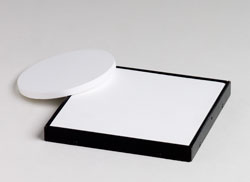
\includegraphics[height=3cm]{./Images/spectralon-web.jpg}
				\end{figure}
				\vspace{-.7cm}
				\begin{figure}[htb]
					\centering
					 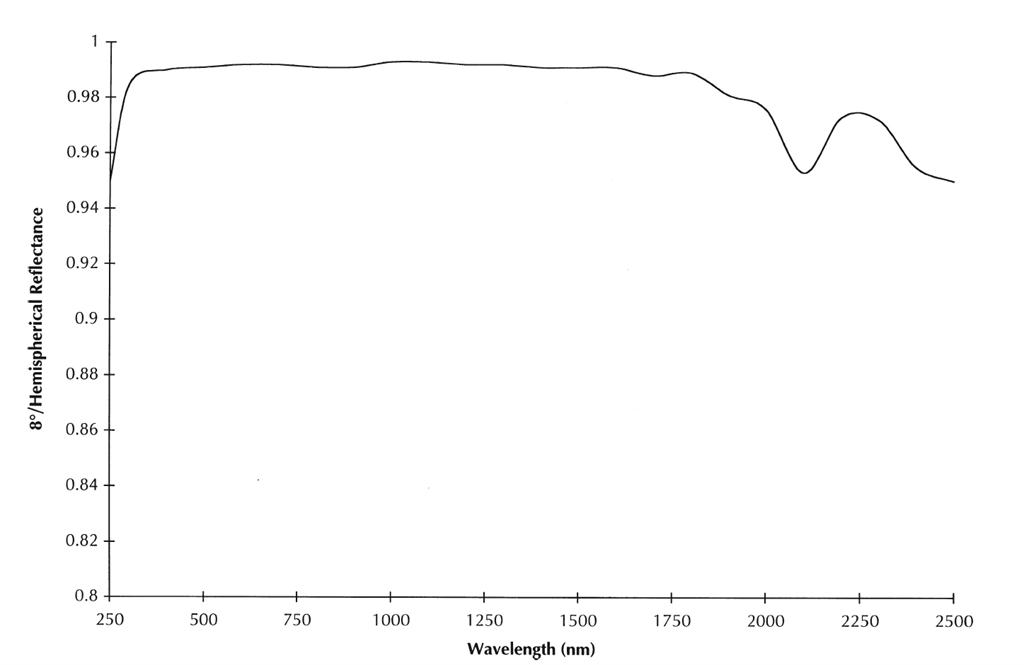
\includegraphics[height=4cm]{./Images/SpectralonTargetsReflectance.jpg}
				\end{figure}
	 
	\end{column}
\end{columns}
\end{frame}

% --- slide ------------------------------------------------
\begin{frame}{Diffuse white reference panel (Spectralon)}
	\scriptsize
%	\begin{flalign}L_\lambda=&
%		\underbrace{E_{s,\lambda}\cdot\cos\sigma\cdot\tau_{1,\lambda}\cdot\tau_{2,\lambda}\cdot\frac{\rho_\lambda}{\pi}}_{\mbox{solar}}+
%		\underbrace{\epsilon_\lambda\cdot\tau_{2,\lambda}\cdot L_{T,\lambda}}_{\mbox{emmissive}}+
%		F\cdot E_{ds,\lambda}\cdot\tau_{2,\lambda}\cdot\frac{r_{d,\lambda}}{\pi}+\nonumber\\
%		&F\cdot E_{d\epsilon,\lambda}\cdot\tau_{2,\lambda}\cdot\frac{r_{d,\lambda}}{\pi}+
%		(1-F)\cdot L_{bs,\lambda}\cdot\tau_{2,\lambda}\cdot r_{d,\lambda}+\nonumber\\
%		&(1-F)\cdot L_{b\epsilon,\lambda}\cdot\tau_{2,\lambda}\cdot r_{d,\lambda}+
%		\underbrace{L_{us,\lambda}+L_{u\epsilon,\lambda}}_{\mbox{upwelling}}
%	\end{flalign}
	\begin{equation}
		L=\underbrace{E_s'\cdot\cos\sigma'\cdot\tau_1\cdot\tau_2\cdot\frac{\rho}{\pi}}_{\mbox{solar}}+
		\underbrace{F\cdot E_{ds}\cdot\tau_2\cdot\frac{\rho_d}{\pi}}_{\mbox{sky}}+
		\underbrace{(1-F)\cdot E_{bs}\cdot\tau_2\cdot\frac{\rho_d}{\pi}}_{\mbox{adjacency}}+
		\underbrace{L_{us}}_{\mbox{upwelling}}
	\end{equation}
	Eqn.\ 4.69 from \cite{schott2007remote}.
	\begin{flalign}
		L=&m\cdot\rho+b\\
		L_{tar}=&m\cdot\rho_{tar}+b\\
		L_{ref}=&m\cdot\rho_{ref}+b\\
		\rho_{tar}=& \frac{L_{tar}-b}{m}\\
		m=&\frac{L_{ref}-b}{\rho_{ref}}\\
		\rho_{tar}=& \frac{L_{tar}-b}{L_{ref}-b}\cdot\rho_{ref}
	\end{flalign}
\end{frame}

% --- slide ------------------------------------------------
\begin{frame}{Reflectance}
\Large
\begin{itemize}\itemsep0.4cm
	\item{ \textbf{Reflectance:} $R(z,\lambda)\equiv \frac{\displaystyle L_u(z,\lambda)}{\displaystyle E_d(z,\lambda)}$}
	\item Two measurements:\\
		\begin{itemize}\itemsep.2cm
		\large
			\item{ $E_d$: Spectralon}
			\item{ $L_u$: Target or sample}
		\end{itemize}
\end{itemize}



\end{frame}
% --- slide ------------------------------------------------
\begin{frame}{\LARGE Remote-Sensing Reflectance}
 	\begin{columns}[c] % contents are top vertically aligned
  		\begin{column}[T]{5cm} % each column can also be its own environment
  		\begin{itemize}
  		\item 3 measurements:
	  		\begin{itemize}
	  			\item {$L_g$ (spectralon)}
	  			\item {$L_t = L_r+L_w$ (water)}
	  			\item {$L_{sky}$}
	  		\end{itemize}
	  	\item{Remote-sensing reflectance:\\
	  			\vspace{-0.5cm}
	  			\begin{gather*} 
	  				R_{rs} = L_w/E_d\\
	  				= (L_t - L_r)/E_d
	  			\end{gather*}\\
	  			with $L_r = 0.028*L_{sky}$}	
	  	
	  	\item {$E_d = L_g*\pi$}
	  	\item {$\phi:$ azimuthal angle}
	  	\item {$\theta:$ zenith angle}
  		\end{itemize}
    	\end{column}
    	\hspace{-1cm}
    	\begin{column}[T]{7cm} % each column can also be its own environment
  			\begin{figure}[htb]
				\centering
				 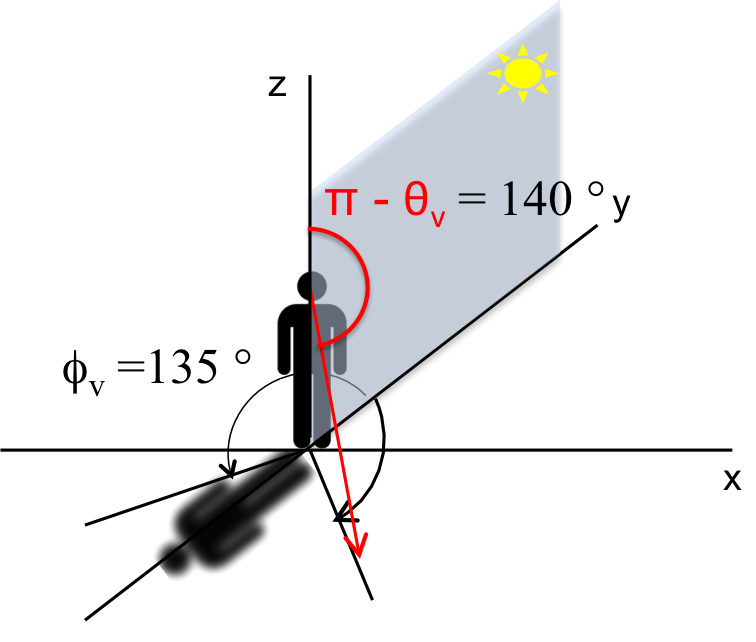
\includegraphics[height=6cm]{./Images/LwGeometry.png}
			\end{figure}
 
    	\end{column}
    \end{columns}
\end{frame}

% --- slide ------------------------------------------------
\begin{frame}{$L_{sky}$}

\begin{figure}[htb]
				\centering
				 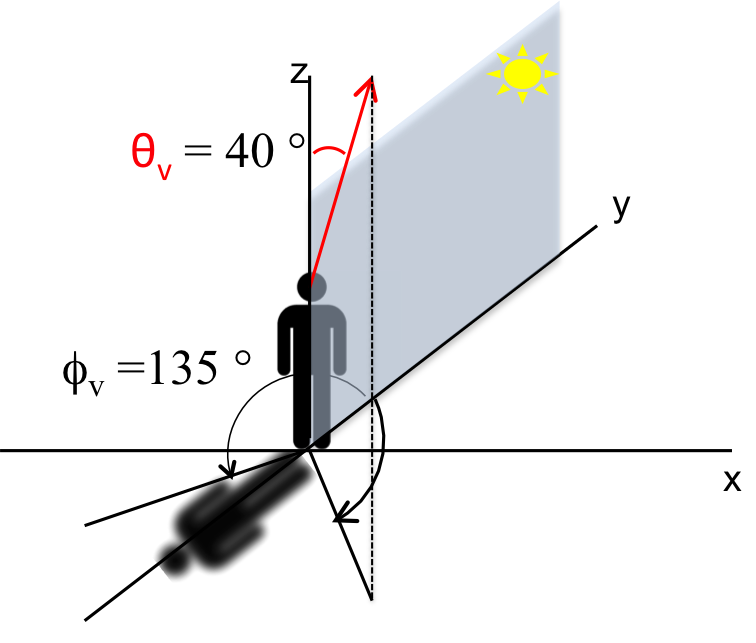
\includegraphics[height=6cm]{./Images/LskyGeometry.png}
			\end{figure}

\end{frame}
% --- slide ------------------------------------------------
\begin{frame}{Things to consider for a field campaign}
\large
\begin{itemize}\itemsep0.35cm
\item Planning ahead: permits, what kind of measurements, how many people, what conditions, instruments availability, shipping, prioritization of data.
\item Equipment check list
\item Contact list: phone numbers, emergency numbers, emails
\item Risk management form (RIT requirement)
\item Direction how to get to the place


\end{itemize}

\end{frame}
% --- slide ------------------------------------------------
\begin{frame}{Things to consider for a field campaign}
\large
\begin{itemize}\itemsep0.35cm
\item Have a good datasheet
\item Download and look data from the instrument ASAP!!!
\item Tools for in-field repairs and cleaning
\item Water, food, field clothes, first aid kit
\item Plan collection ahead of time
\item Write down procedure
\item Setting up plots/sites
\item Take pictures

\end{itemize}

\end{frame}
% --- slide ------------------------------------------------
\begin{frame}{Things to consider for a field campaign}
\large
\begin{itemize}\itemsep0.35cm

\item Read instrument manual
\item Check and charge batteries in advance
\item Check instrument in advance
\item The data should be taken as close to the time of acquisition as possible (due to inevitable landscape changes)
\item Weather conditions 
\item Take measurement in same illumination conditions

\end{itemize}

\end{frame}
%%%%%%%%%%%%%%%%%%% SECTION %%%%%%%%%%%%%%%%%%%%%%%%%%%%%%%%
\section{DIRS Instruments}
\subsection*{}
% --- slide ------------------------------------------------
\begin{frame}{DIRS Lab Instruments}
\large
\begin{itemize}\itemsep.4cm
	\item ASD (Spectroradiometer; reflectance, radiance)
	\item SVC (Spectroradiometer; reflectance, radiance)
	\item RIT LIDAR
	\item GRIT (Goniometer; BRDF)
	\item GPS (Location)
	\item HydroScat-2 (Backscattering)
	\item AccuPAR LP-80 (PAR energy)
\end{itemize}

\end{frame}
% --- slide ------------------------------------------------
\begin{frame}{DIRS Lab Instruments (con't)}
\large
\begin{itemize}\itemsep.4cm
	\item WASP (Multispectral Instrument)
	\item WASP Lite (Multispectral Instrument)
	\item MISI (Multispectral Instrument)
	\item Thermistor (Temperature)
	\item Spectrophotometer (Absorbance)
	\item Camera
\end{itemize}

\end{frame}
% --- slide ------------------------------------------------
\begin{frame}{DIRS Lab Instruments (con't)}{ASD}

 	\begin{columns}[c] % contents are top vertically aligned
  		\begin{column}[T]{5cm} % each column can also be its own environment
		\vspace{1cm}
  		\begin{itemize}\itemsep.4cm
  		\item FieldSpec 4 Spectroradiometer
  		\item Spectral Range: 350-2500 nm (UV, VIS, NIR and SWIR)
  		\item Sampling Interval:	
	  		\begin{itemize}
	  			\item 1.4 nm (350-1000 nm)\\
				\item 2 nm (100-2500 nm)
			\end{itemize}
  		\end{itemize}
    	\end{column}
    	\hspace{-1cm}
    	\begin{column}[T]{7cm} % each column can also be its own environment
  			\begin{figure}[htb]
				\centering
				 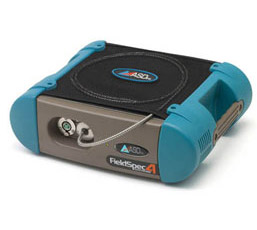
\includegraphics[height=3cm]{./Images/ASD.jpg}
			\end{figure}
			\vspace{-.5cm}
			\begin{figure}[htb]
				\centering
				 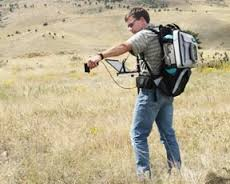
\includegraphics[height=3cm]{./Images/ASDperson.jpeg}
			\end{figure}
 
    	\end{column}
    \end{columns}
\end{frame}
% --- slide ------------------------------------------------
\begin{frame}{DIRS Lab Instruments (con't)}{SVC}

 	\begin{columns}[c] % contents are top vertically aligned
  		\begin{column}[T]{5cm} % each column can also be its own environment
		\vspace{1cm}
  		\begin{itemize}\itemsep.4cm
  		\item Spectra Vista Corp. (SVC) Spectroradiometer
  		\item Spectral Range: 350-2500 nm (UV, VIS, NIR and SWIR)
  		\item Sampling Interval: 
	  		\begin{itemize}
	  			\item 1.5 nm, 350-1000 nm\\ 
				\item 3.8 nm, 1000-1890 nm\\ 
				\item 9.5 nm, 1890-2500 nm
			\end{itemize}
  		\end{itemize}
    	\end{column}
    	\hspace{-1cm}
    	\begin{column}[T]{7cm} % each column can also be its own environment
  			\begin{figure}[htb]
				\centering
				 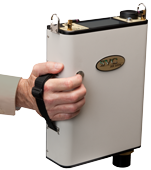
\includegraphics[height=3cm]{./Images/1024i-Unit.png}
			\end{figure}
			\vspace{-.5cm}
			\begin{figure}[htb]
				\centering
				 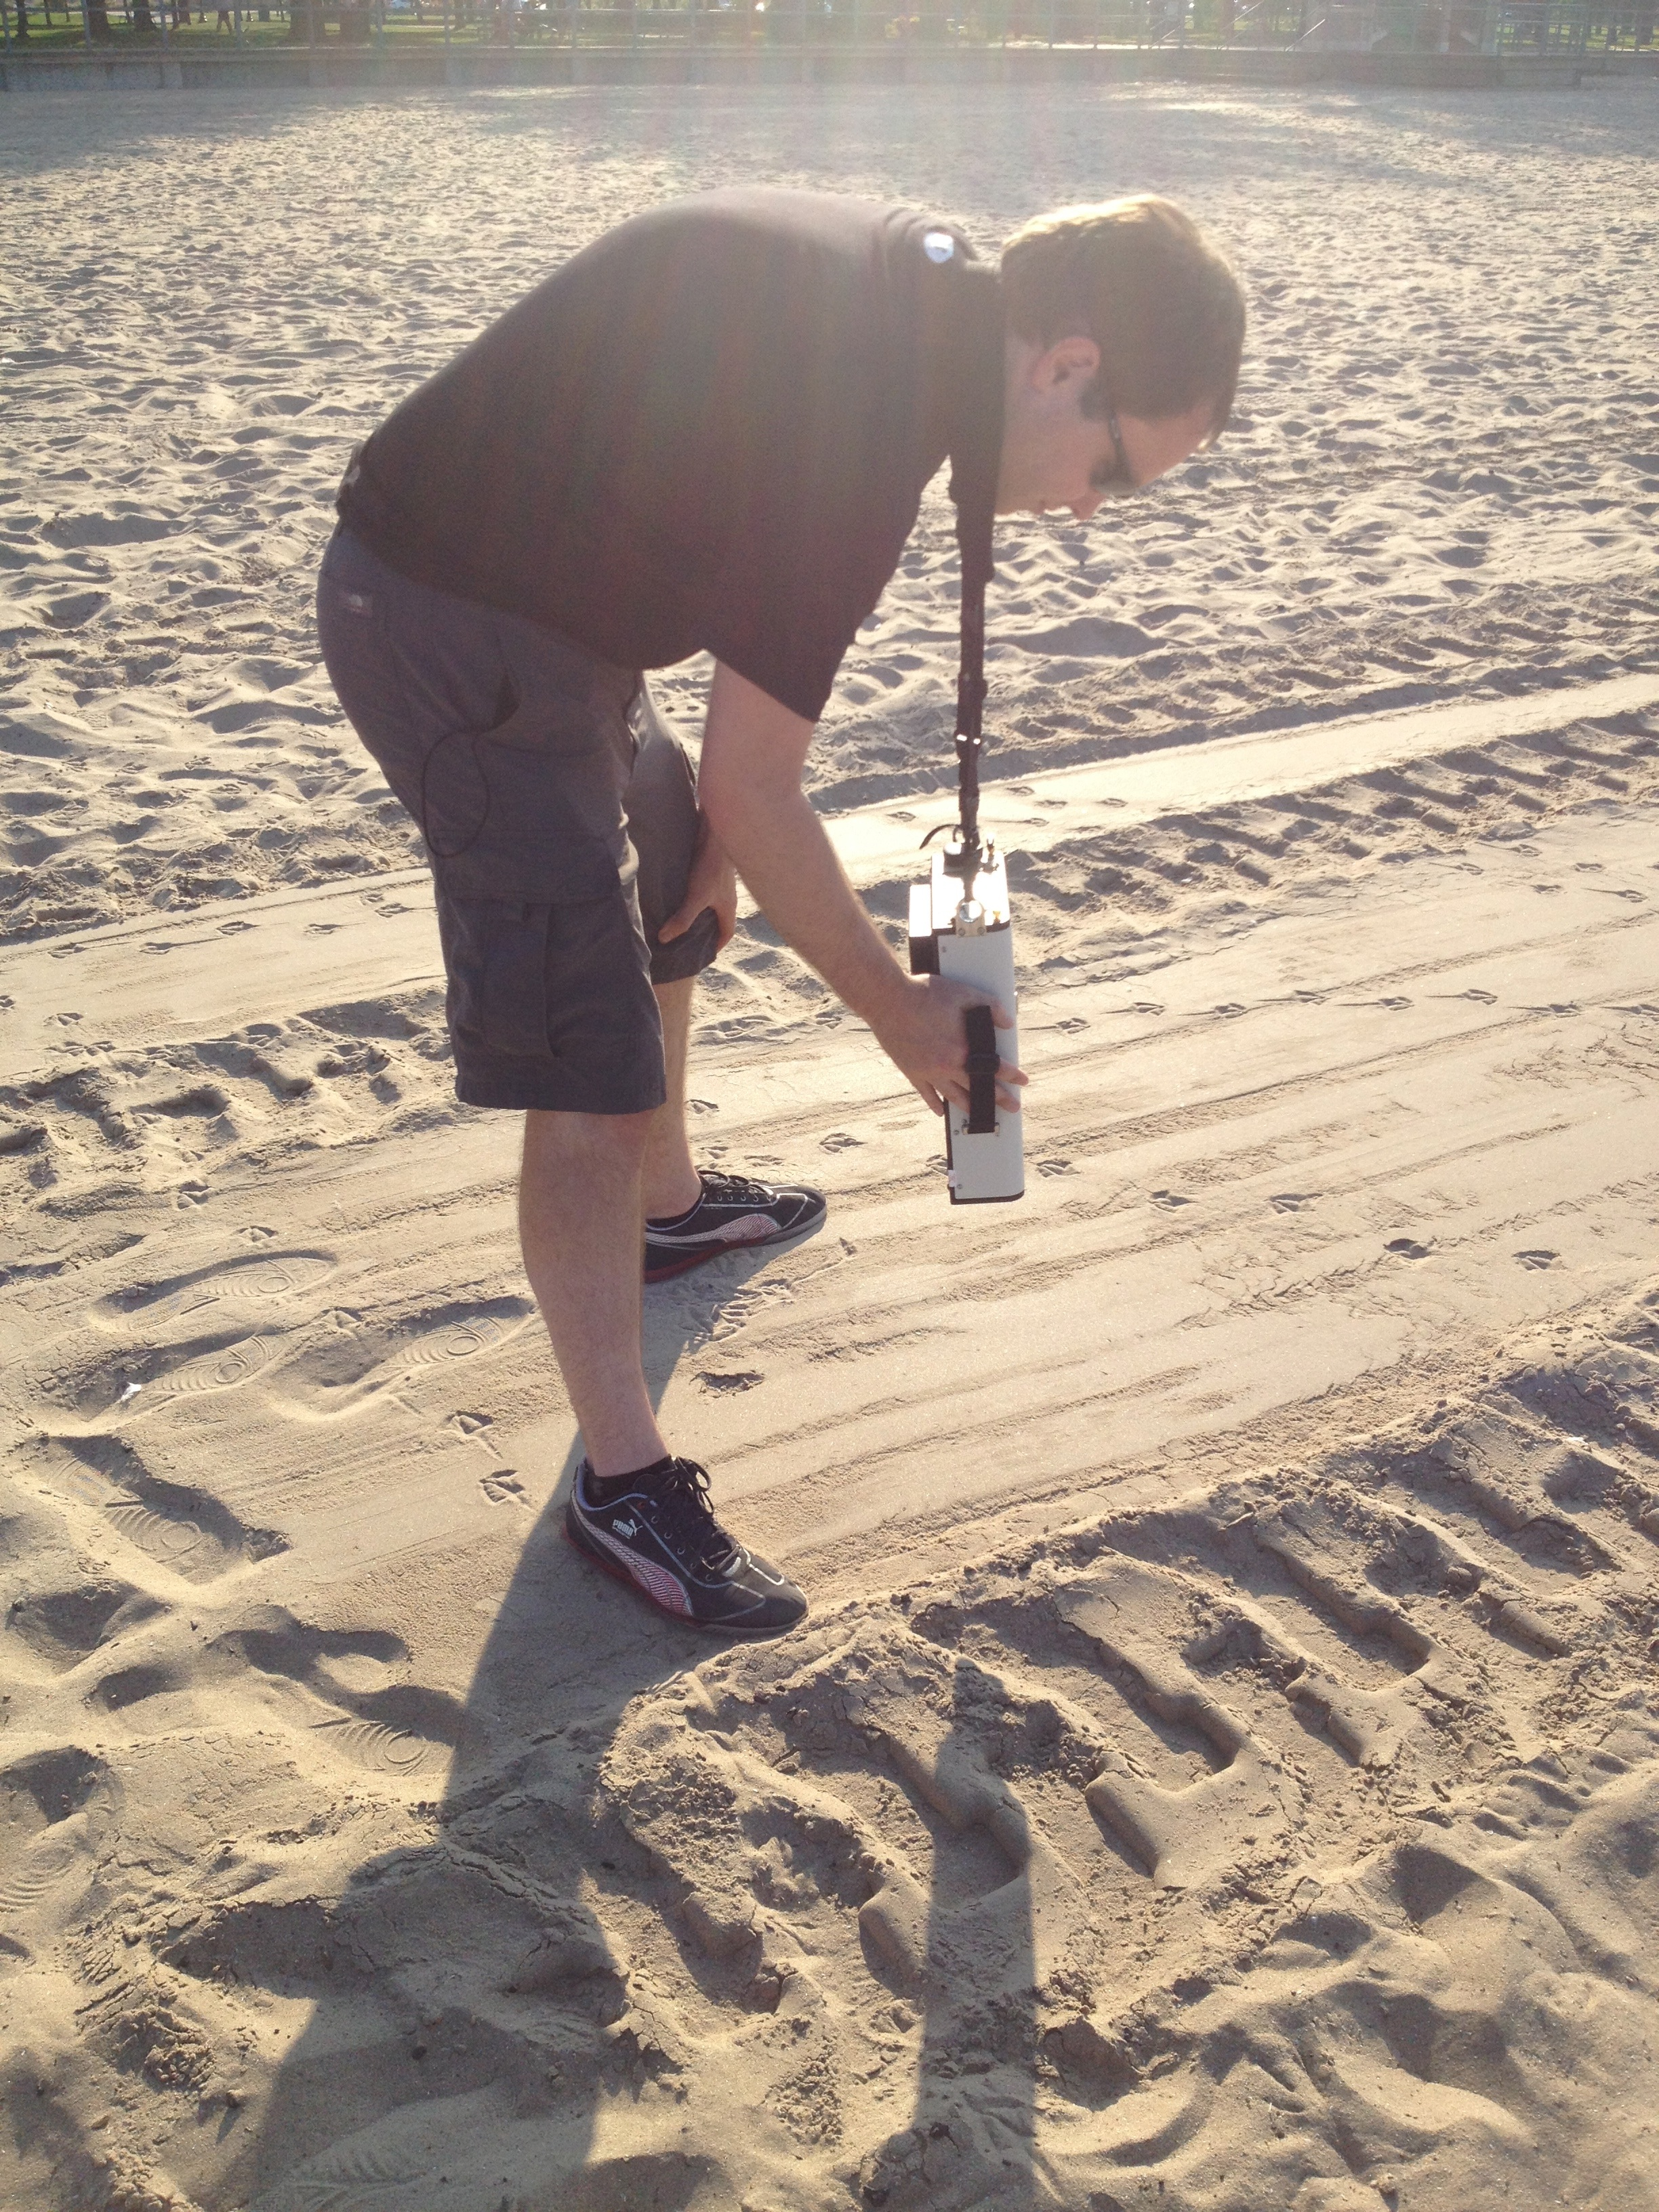
\includegraphics[height=3cm]{./Images/PaulSand.jpg}
			\end{figure}
 
    	\end{column}
    \end{columns}
\end{frame}
% --- slide ------------------------------------------------
\begin{frame}{DIRS Lab Instruments (con't)}{LIDAR}
 	\begin{columns}[c] % contents are top vertically aligned
  		\begin{column}[T]{5cm} % each column can also be its own environment
  		\vspace{1cm}
  		\begin{itemize}\itemsep.4cm
  		\item Light Detection and Ranging (LiDAR)
  		\item Similar to RADAR but it uses laser light.
  		\item Generate 3D models of the environment
  		\end{itemize}
    	\end{column}
    	\hspace{-1cm}
    	\begin{column}[T]{7cm} % each column can also be its own environment
    		\vspace{-.5cm}
  			\begin{figure}[htb]
				\centering
				 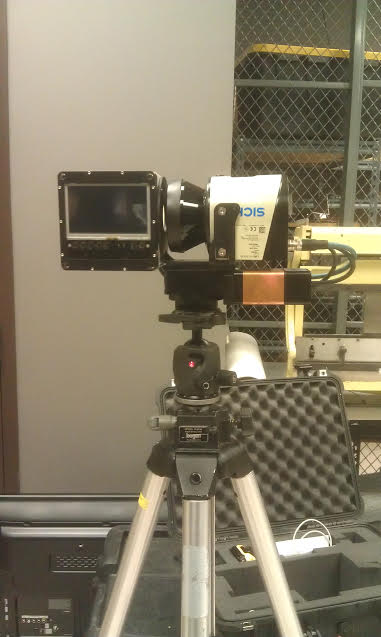
\includegraphics[height=4cm]{./Images/LidarRIT.jpg}
			\end{figure}
			\vspace{-.5cm}
			\begin{figure}[htb]
				\centering
				 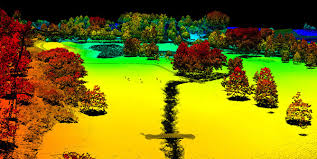
\includegraphics[height=2cm]{./Images/Lidar3D.jpeg}
			\end{figure}
			
 
    	\end{column}
    \end{columns}
\end{frame}
%%%%%%%%%%%%%%%%%%% SECTION %%%%%%%%%%%%%%%%%%%%%%%%%%%%%%%%
\section{Data Processing}
\subsection*{}
% --- slide ------------------------------------------------
\begin{frame}{Data Extraction}
\Large
\begin{itemize}\itemsep.4cm
	\item Raw data in proprietary format (depending of the instrument). Ex: *.dat, *.SPC
	\item Translate or export to ASCII (*.txt, *.ASC)
	\item Text files manipulation (IDL, Matlab, Python, C++, bash).
\end{itemize}



\end{frame}
% --- slide ------------------------------------------------
\begin{frame}{Data in ASCII format}{ASD}

\begin{figure}
\centering
    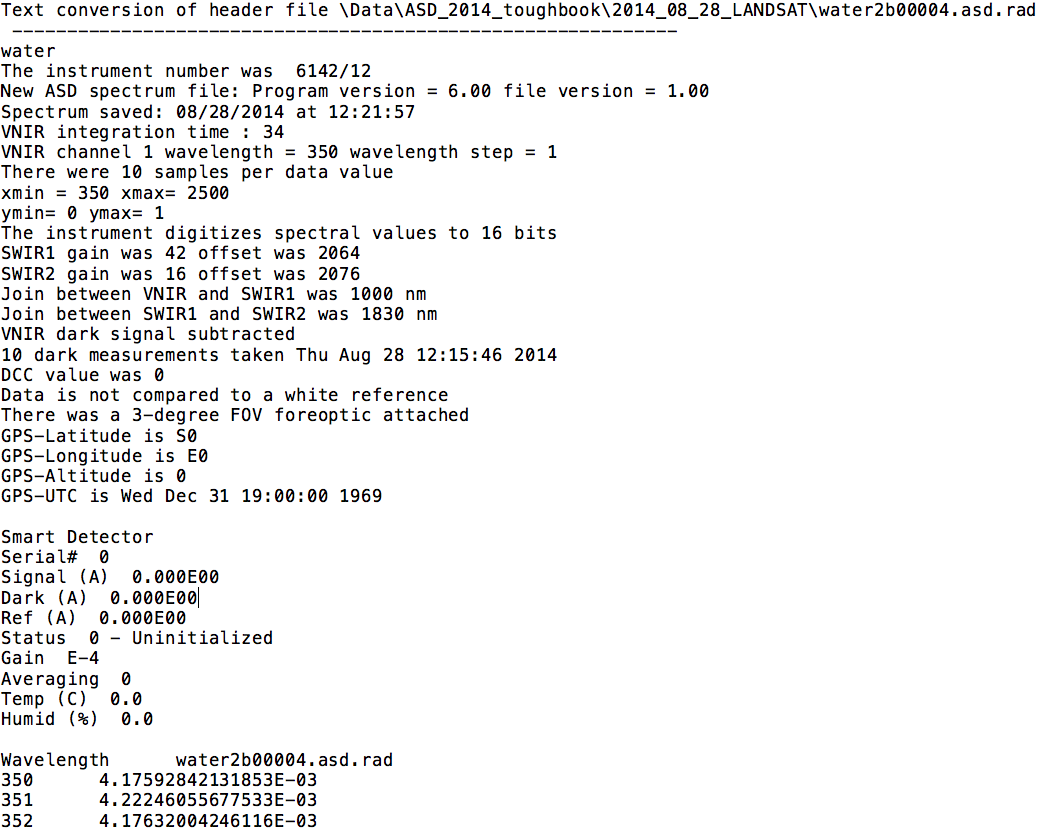
\includegraphics[height=7cm]{./Images/TextFileASD.png}
\end{figure}

\end{frame}
% --- slide ------------------------------------------------
\begin{frame}{Data in ASCII format}{SVC}
\vspace{-.5cm}
\begin{figure}
\centering
    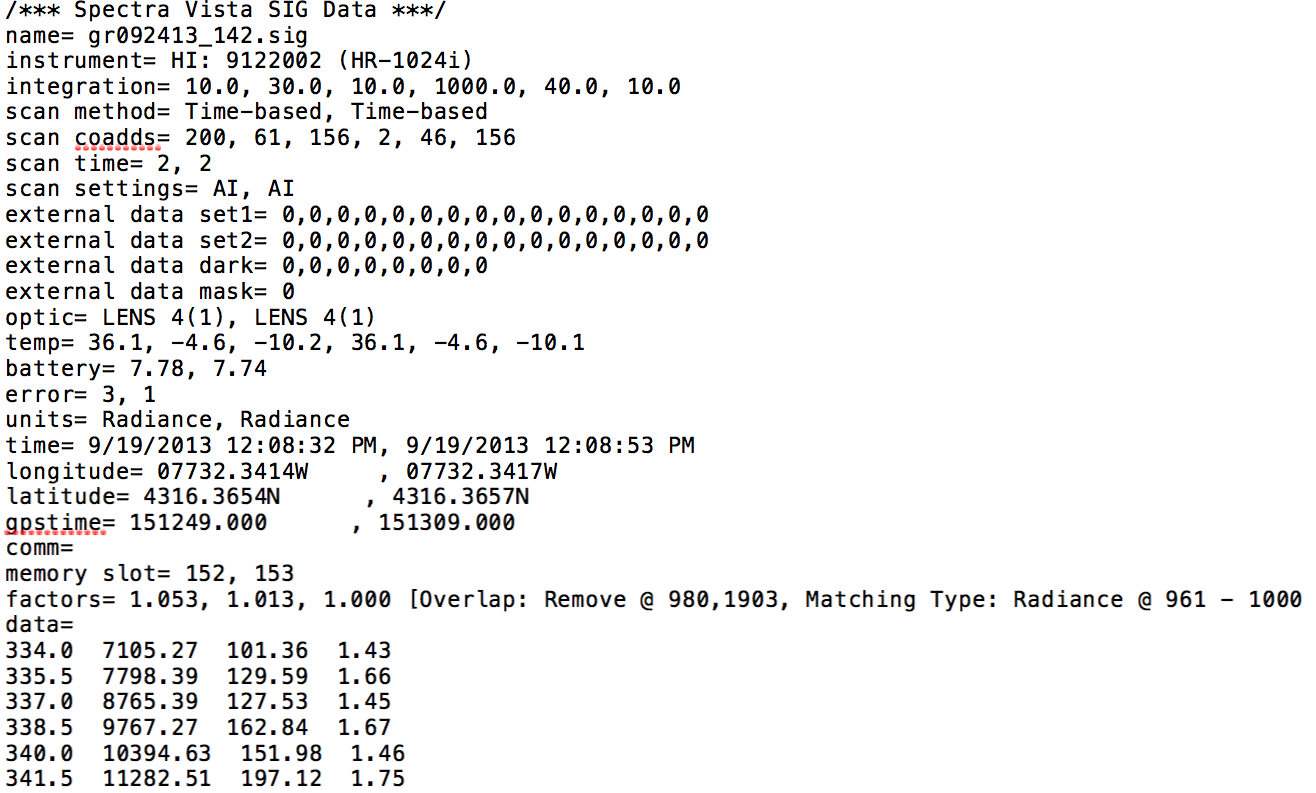
\includegraphics[height=7cm]{./Images/TextFileSVC.png}
\end{figure}

\end{frame}
% --- slide ------------------------------------------------
\begin{frame}{Text files manipulation}{SVC}
\begin{figure}
\centering
    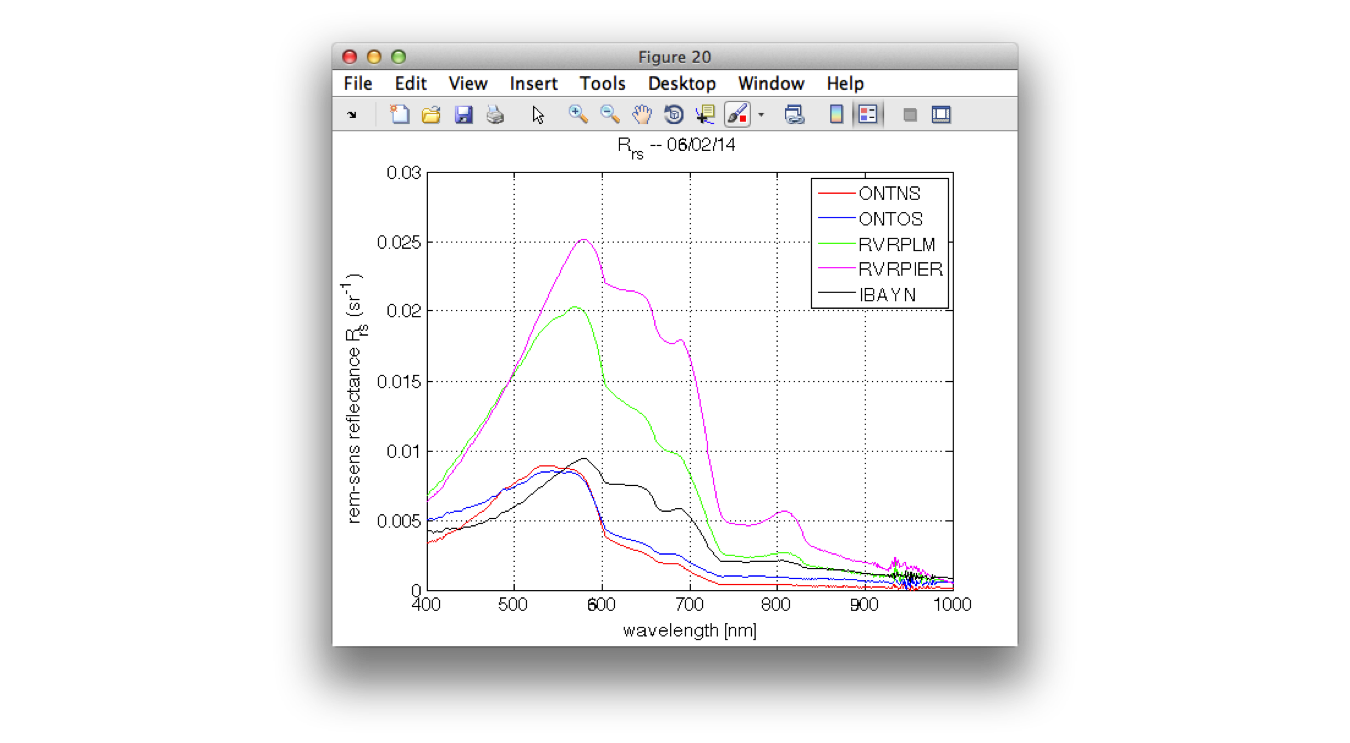
\includegraphics[height=6.5cm]{./Images/Reflectances.png}
\end{figure}

\end{frame}
%%%%%%%%%%%%%%%%%%% SECTION %%%%%%%%%%%%%%%%%%%%%%%%%%%%%%%%
\section{Conclusions}
\subsection*{}
% --- slide ------------------------------------------------
\begin{frame}{Field Campaigns }
\Large

\begin{itemize}
	\item Negative

	\begin{itemize}\itemsep.1cm
	\large
		\item Weather dependent
		\item Extreme environmental conditions (too cold or too hot)
		\item Instrumentation failure
		\item Long days
	\end{itemize}

	\item Positive

	\begin{itemize}\itemsep.1cm
	\large
		\item Brings theory to practice
		\item Appreciate nature (nice to be outside your office)
		\item Get to know more about your colleagues
		\item Know new places
		\item It is FUN!
	\end{itemize}	
\end{itemize}

\end{frame}

%%%%%%%%%%%% Paul's %%%%%%%%%%%%

% --- slide ------------------------------------------------
\begin{frame}{Field Campaigns in Pictures}
\vspace{-.5cm}
\begin{figure}
\centering
    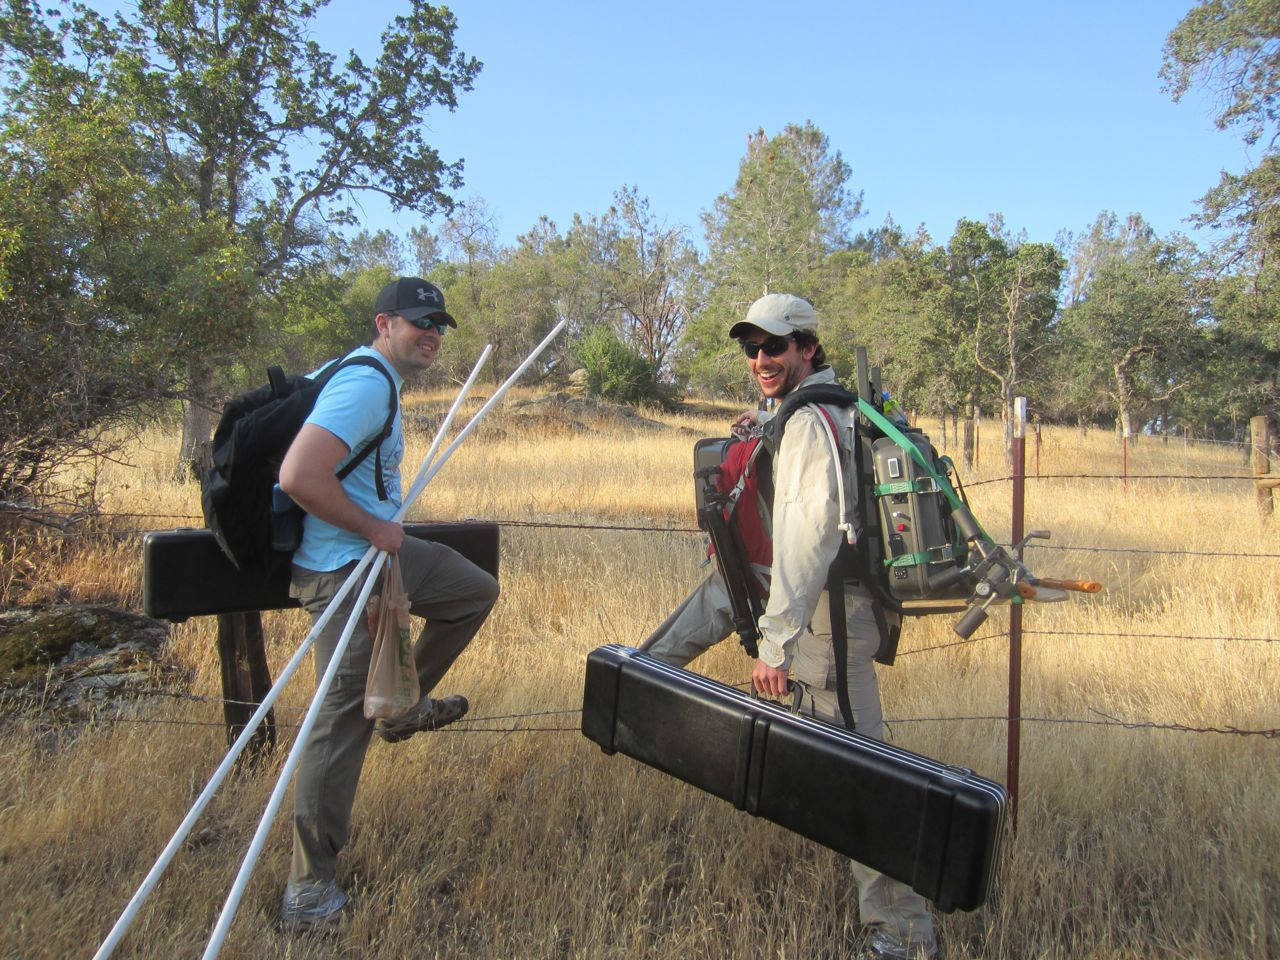
\includegraphics[height=7cm]{./Images/06}
\end{figure}
\end{frame}
% --- slide ------------------------------------------------
\begin{frame}{Field Campaigns in Pictures}
\vspace{-.5cm}
\begin{figure}
\centering
    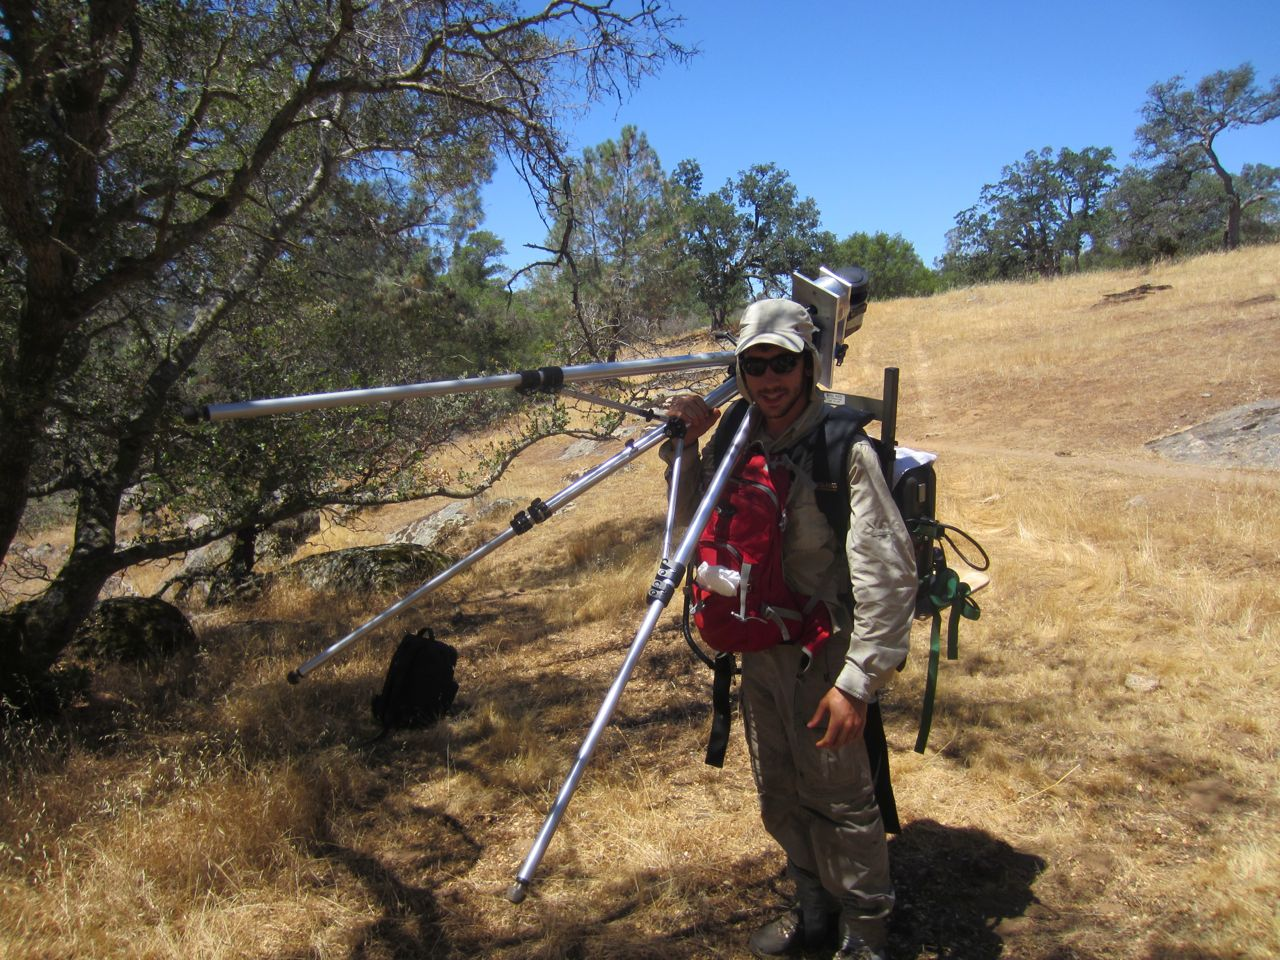
\includegraphics[height=7cm]{./Images/07}
\end{figure}
\end{frame}
% --- slide ------------------------------------------------
\begin{frame}{Field Campaigns in Pictures}
\vspace{-.5cm}
\begin{figure}
\centering
    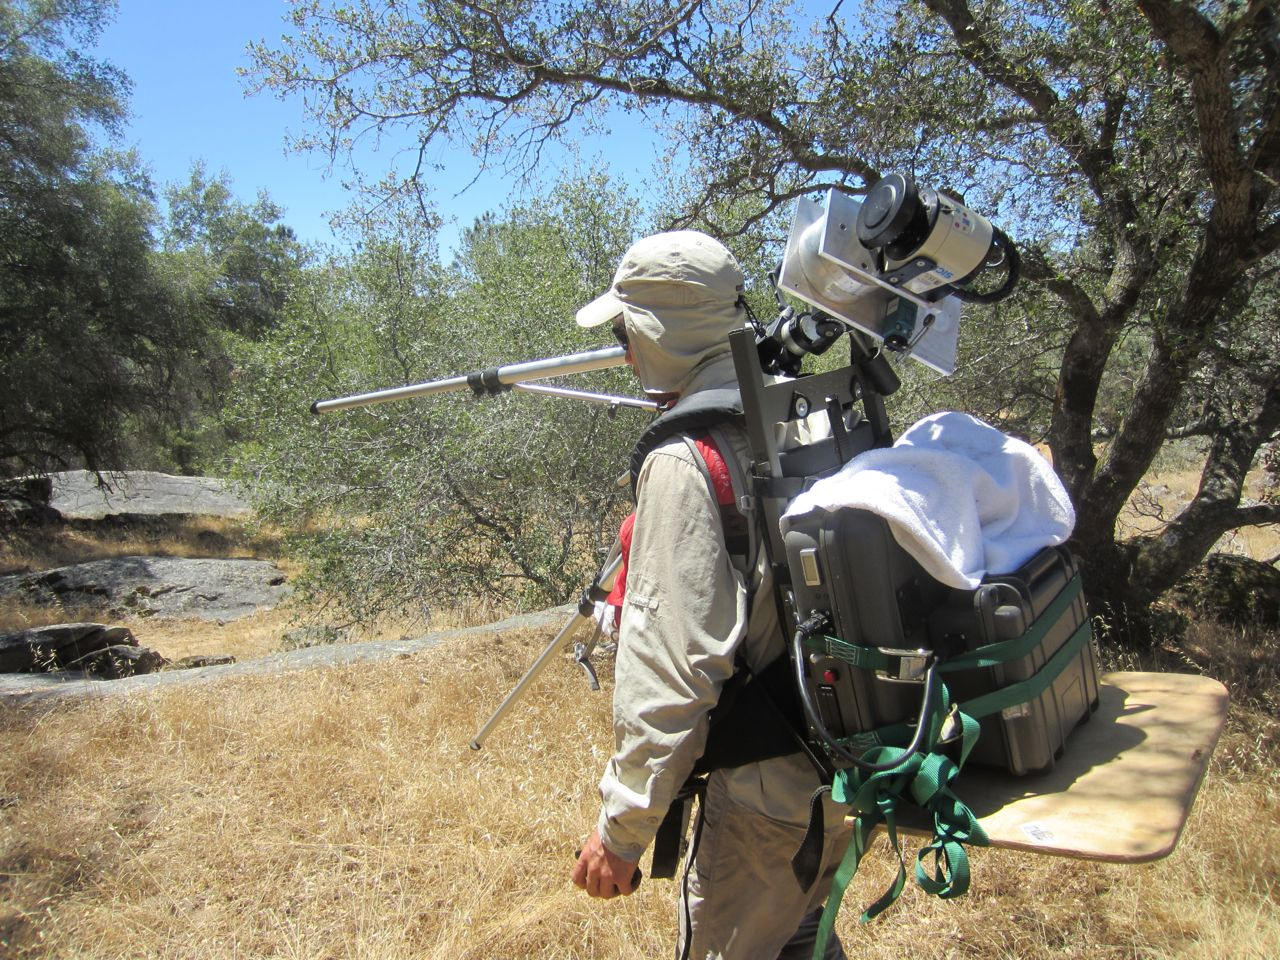
\includegraphics[height=7cm]{./Images/09}
\end{figure}
\end{frame}
% --- slide ------------------------------------------------
\begin{frame}{Field Campaigns in Pictures}
\vspace{-.5cm}
\begin{figure}
\centering
    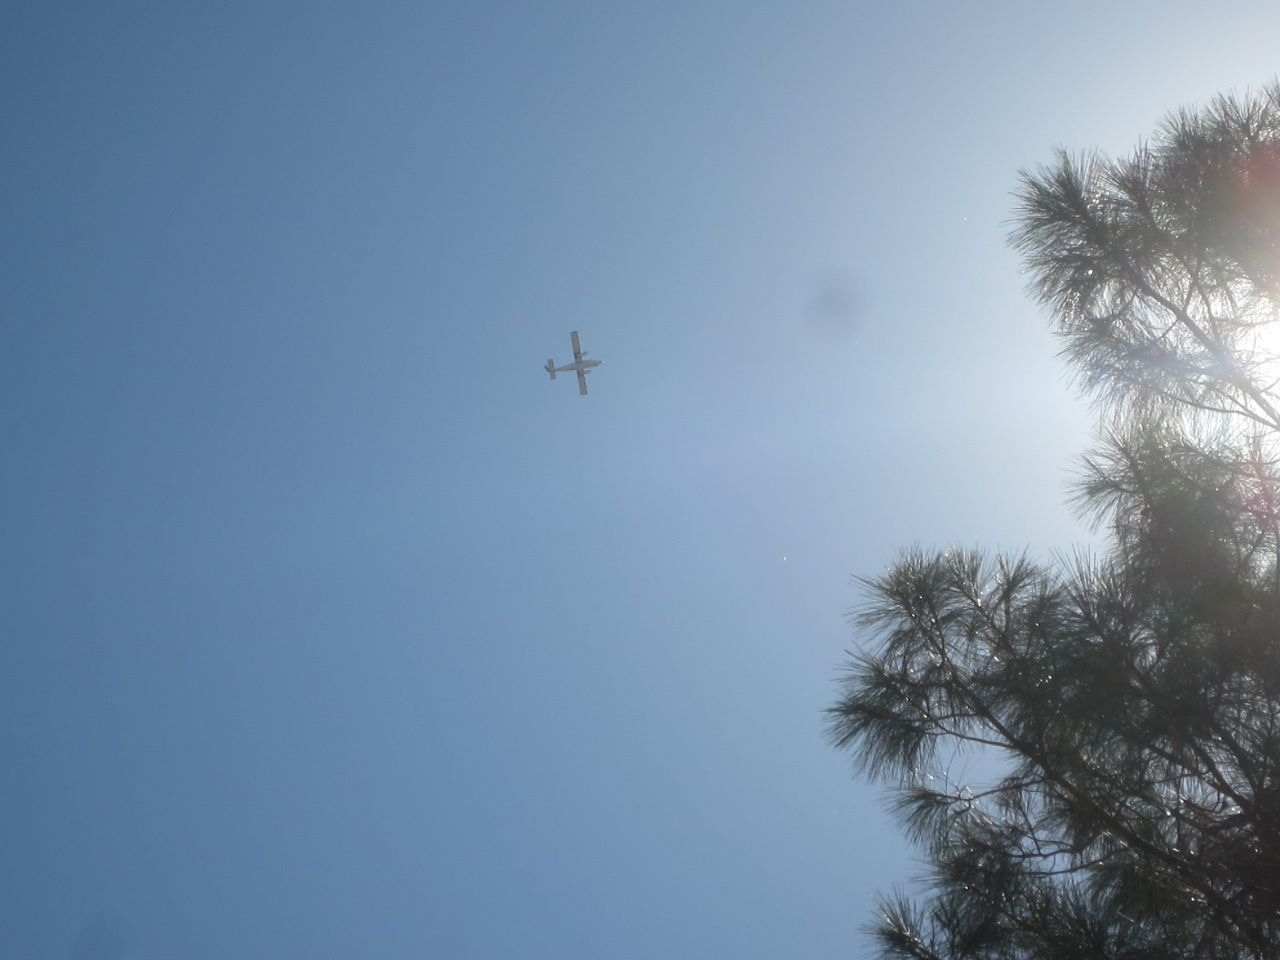
\includegraphics[height=7cm]{./Images/11}
\end{figure}
\end{frame}
% --- slide ------------------------------------------------
\begin{frame}{Field Campaigns in Pictures}
\vspace{-.5cm}
\begin{figure}
\centering
    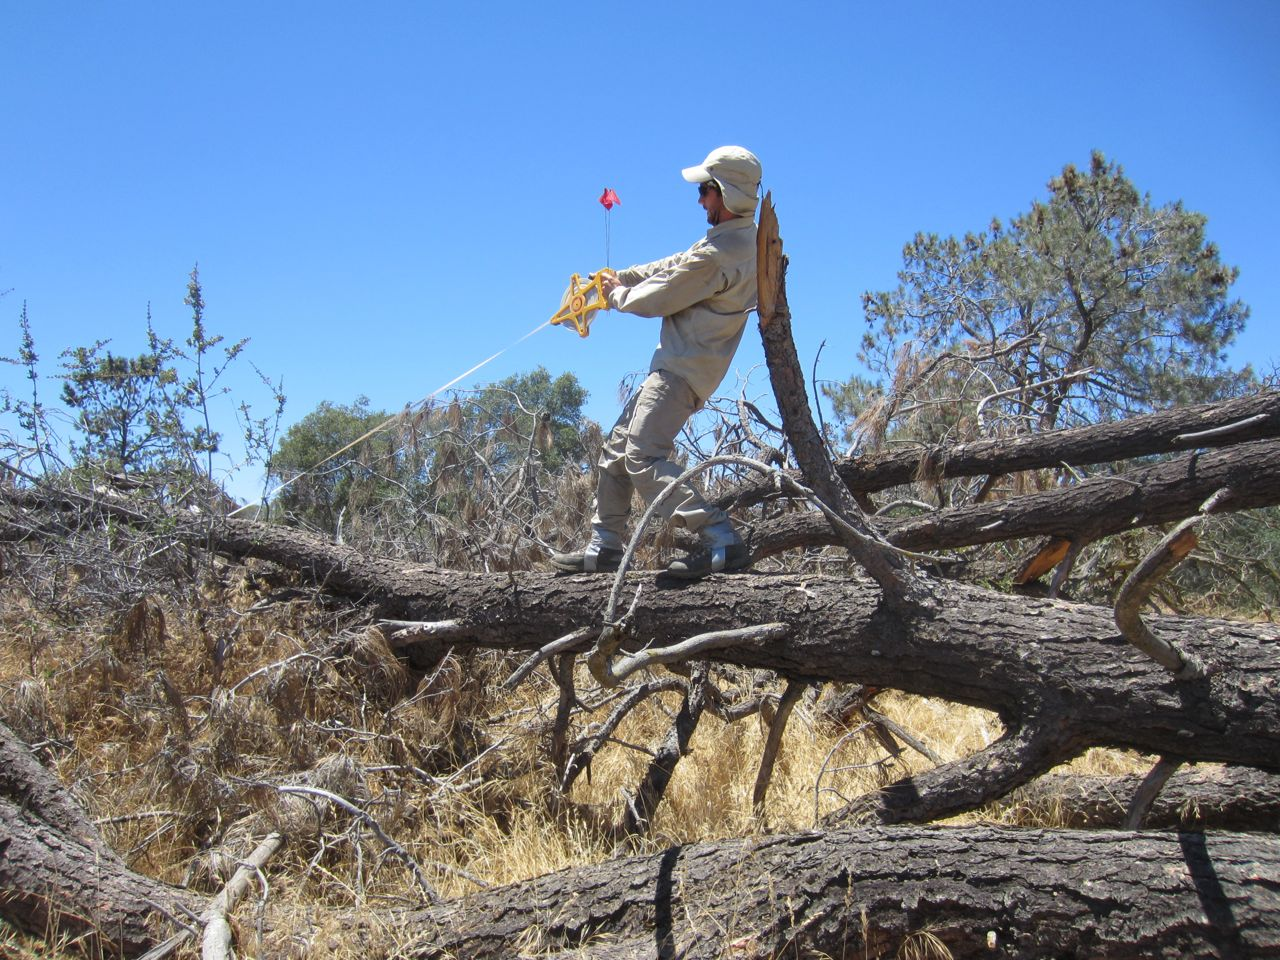
\includegraphics[height=7cm]{./Images/16}
\end{figure}
\end{frame}
% --- slide ------------------------------------------------
\begin{frame}{Field Campaigns in Pictures}
\vspace{-.5cm}
\begin{figure}
\centering
    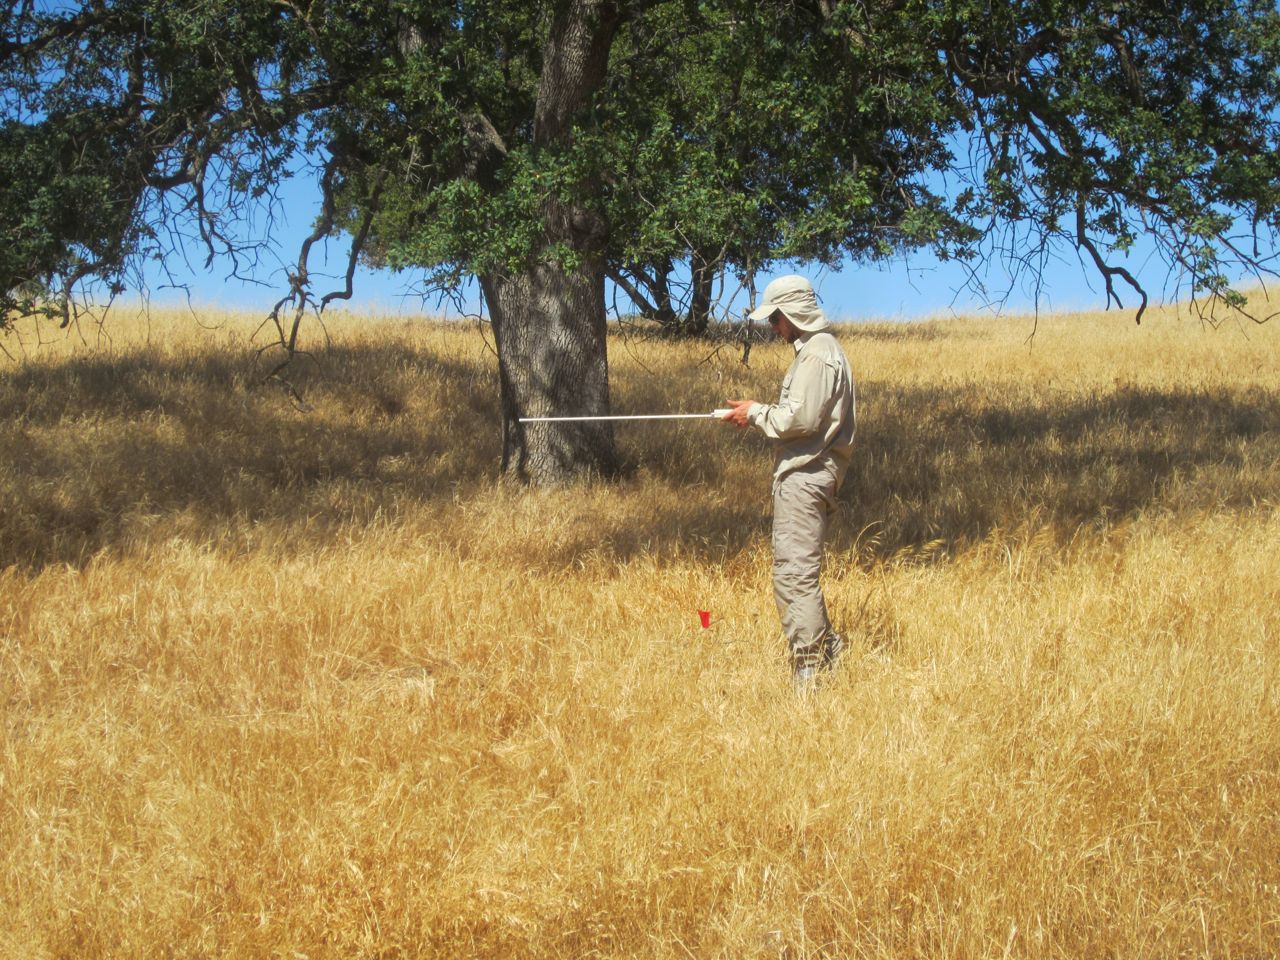
\includegraphics[height=7cm]{./Images/20}
\end{figure}
\end{frame}
% --- slide ------------------------------------------------
\begin{frame}{Field Campaigns in Pictures}
\vspace{-.5cm}
\begin{figure}
\centering
    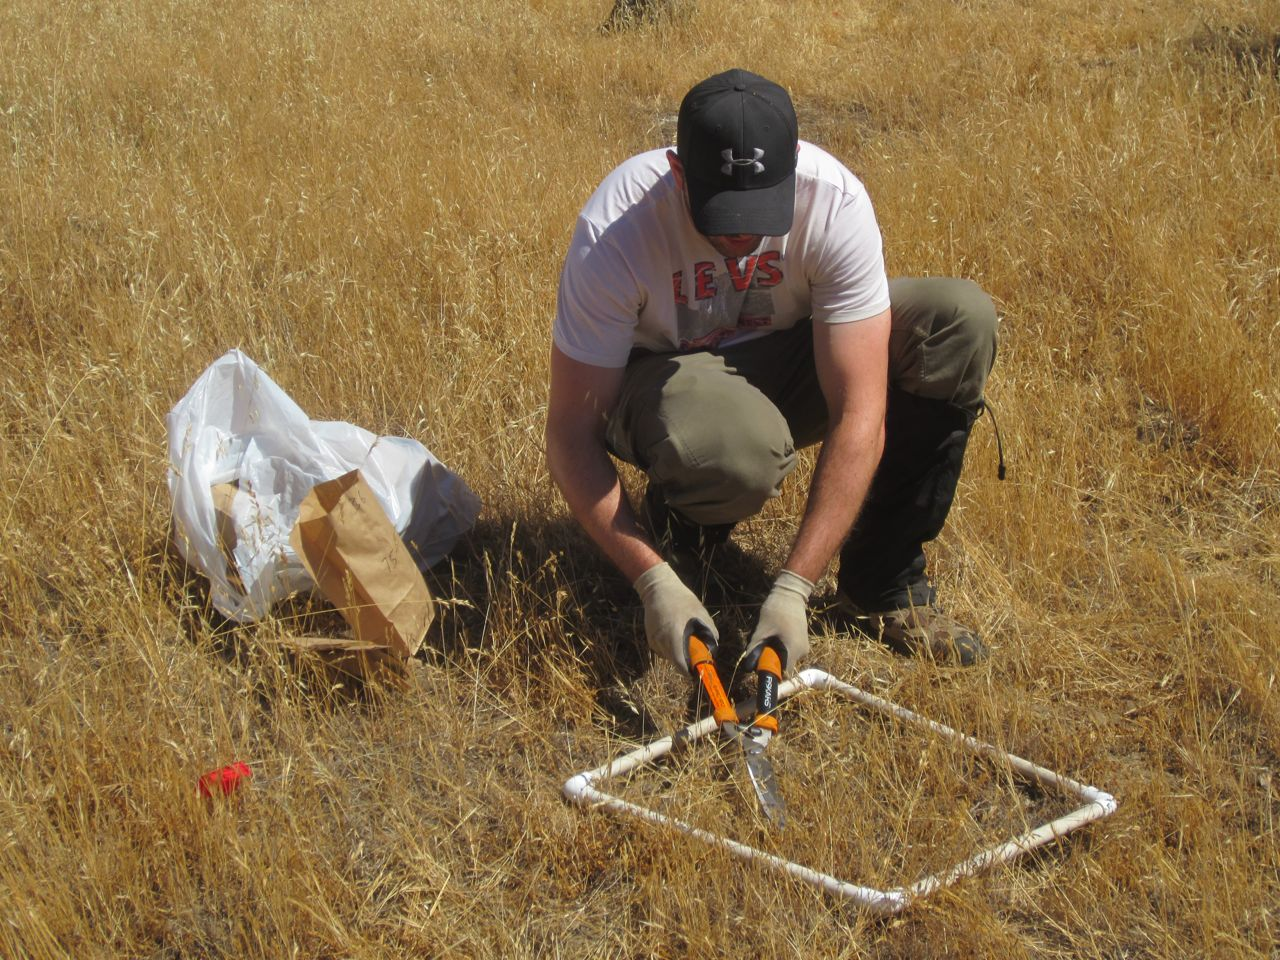
\includegraphics[height=7cm]{./Images/21}
\end{figure}
\end{frame}
% --- slide ------------------------------------------------
\begin{frame}{Field Campaigns in Pictures}
\vspace{-.5cm}
\begin{figure}
\centering
    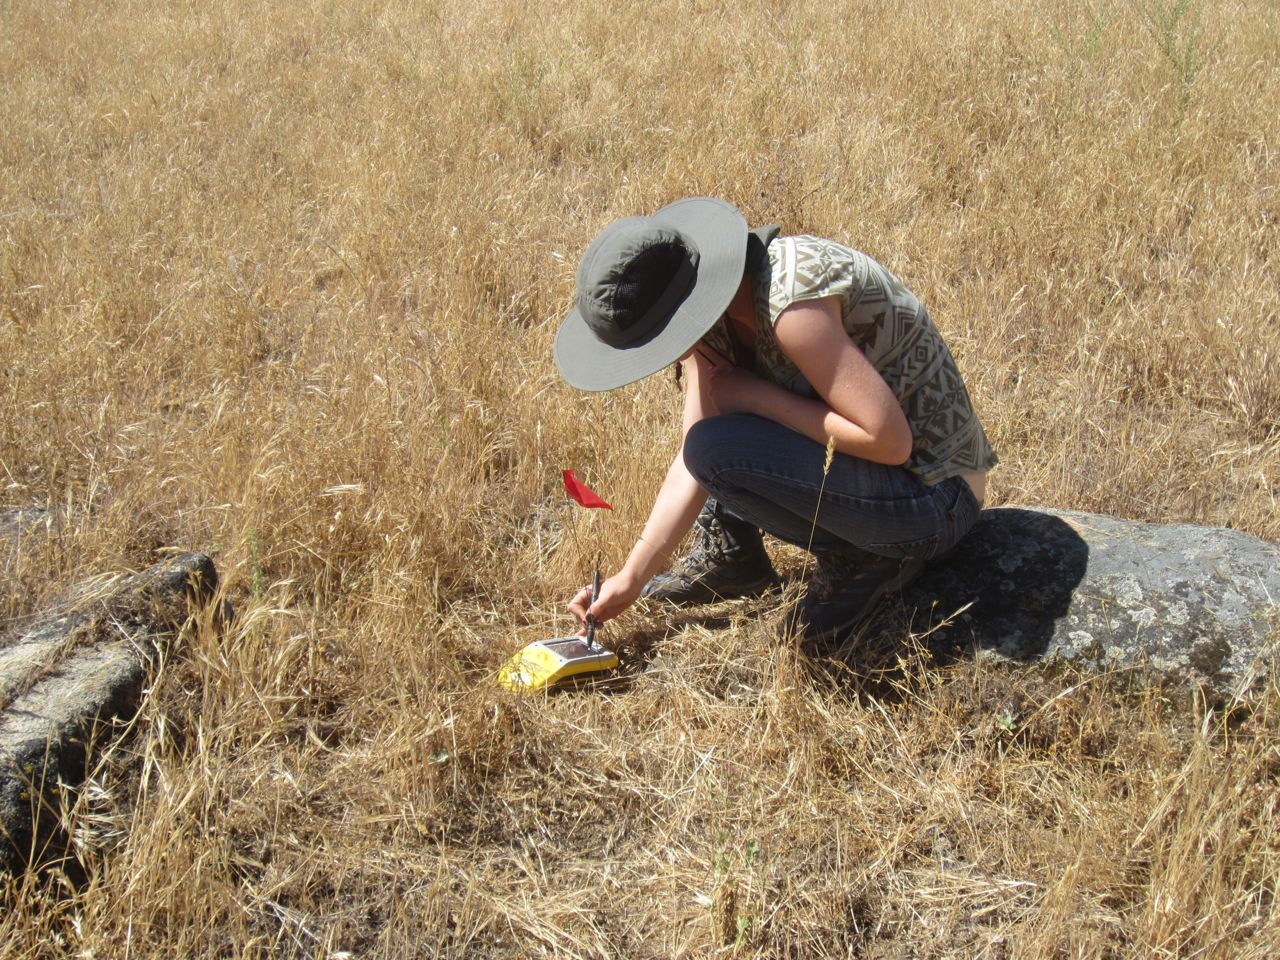
\includegraphics[height=7cm]{./Images/22}
\end{figure}
\end{frame}
% --- slide ------------------------------------------------
\begin{frame}{Field Campaigns in Pictures}
\vspace{-.5cm}
\begin{figure}
\centering
    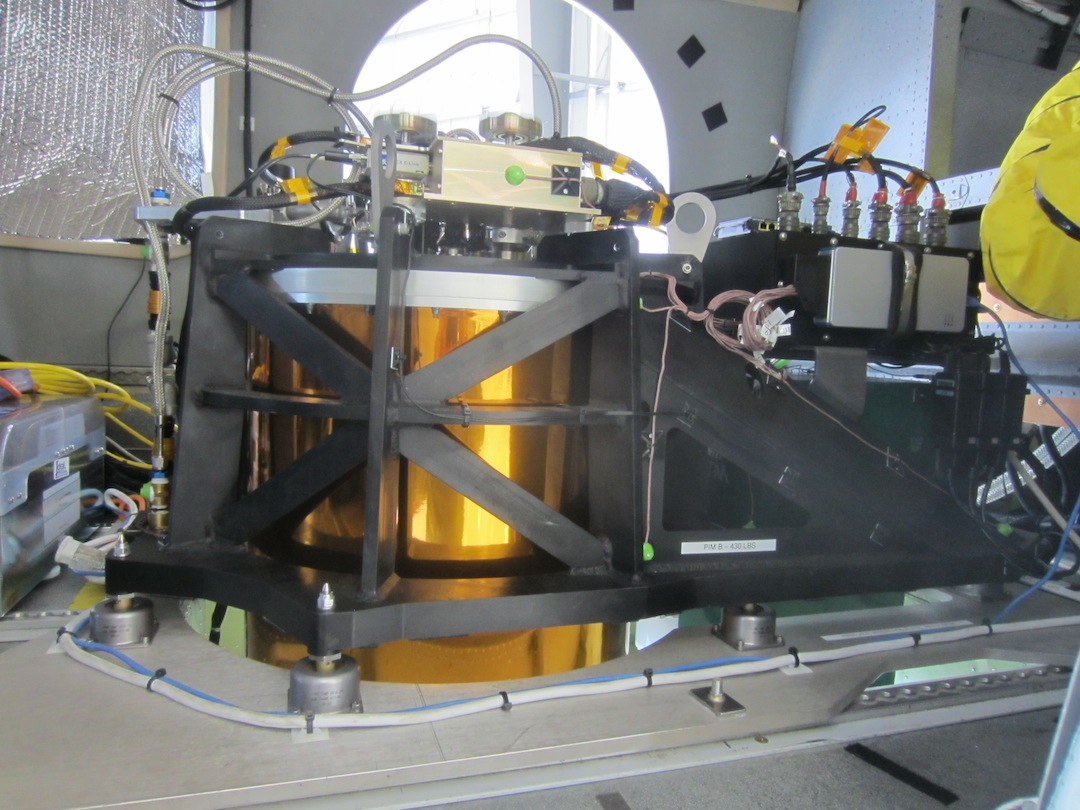
\includegraphics[height=7cm]{./Images/IMG_5878}
\end{figure}
\end{frame}
% --- slide ------------------------------------------------
\begin{frame}{Field Campaigns in Pictures}
\vspace{-.5cm}
\begin{figure}
\centering
    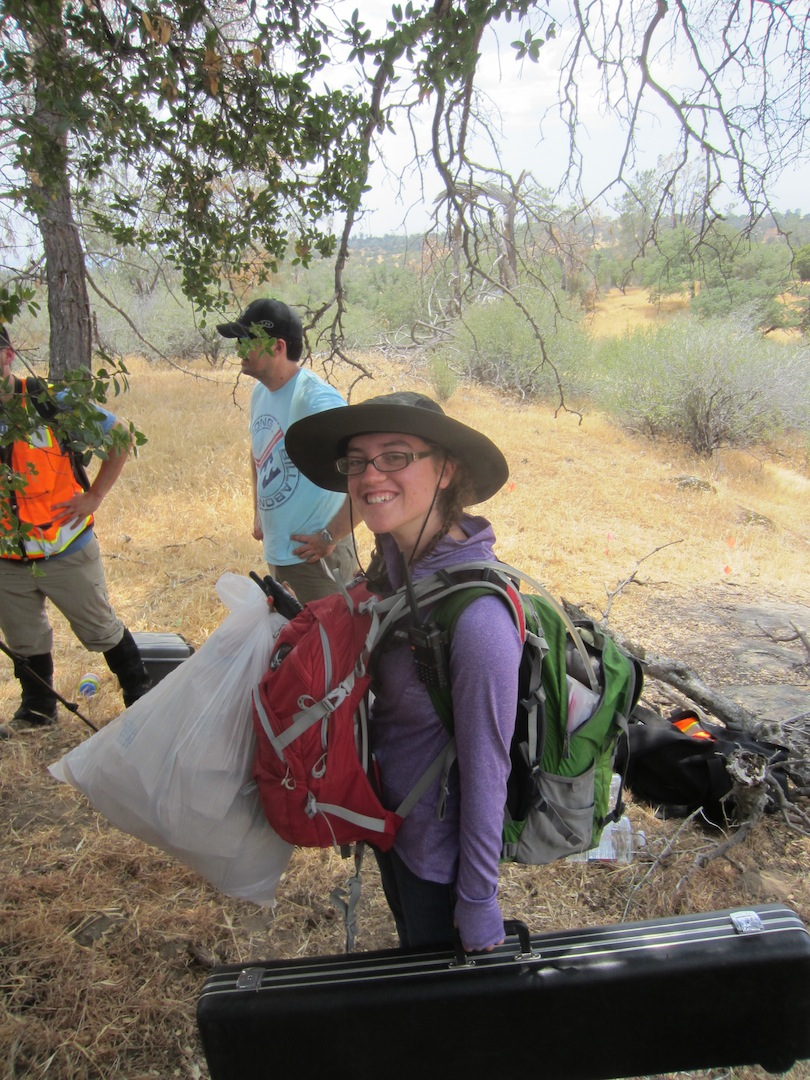
\includegraphics[height=7cm]{./Images/IMG_5897}
\end{figure}
\end{frame}
% --- slide ------------------------------------------------
\begin{frame}{Field Campaigns in Pictures}
\vspace{-.5cm}
\begin{figure}
\centering
    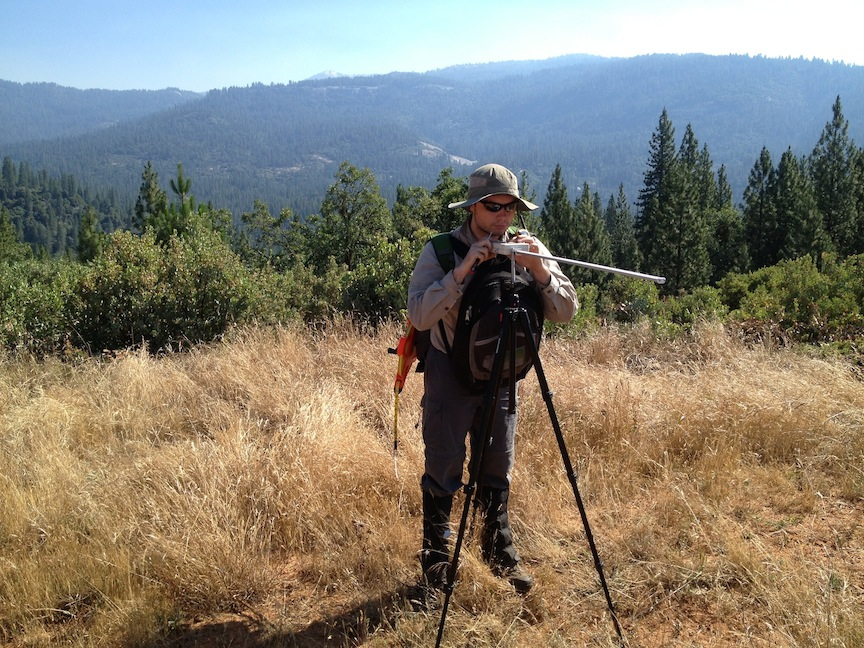
\includegraphics[height=7cm]{./Images/IMG_1710}
\end{figure}
\end{frame}
% --- slide ------------------------------------------------
\begin{frame}{Field Campaigns in Pictures}
\vspace{-.5cm}
\begin{figure}
\centering
    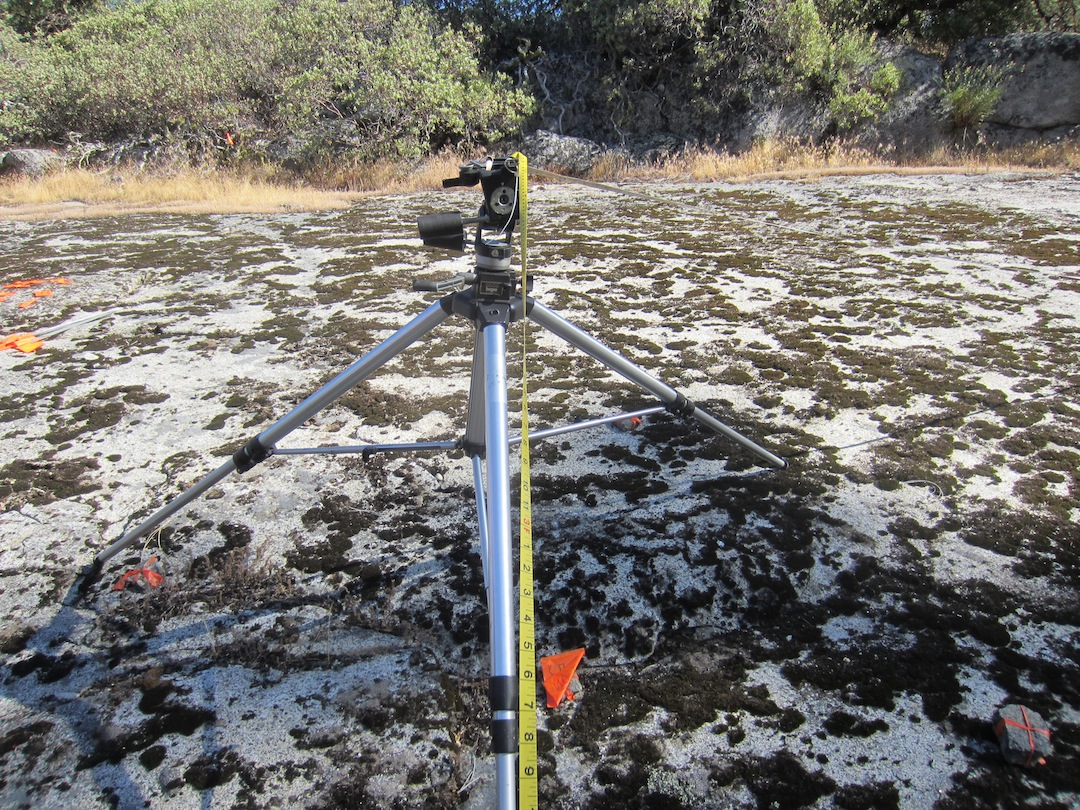
\includegraphics[height=7cm]{./Images/IMG_6484}
\end{figure}
\end{frame}

% --- slide ------------------------------------------------
\begin{frame}{Field Campaigns in Pictures}
\vspace{-.5cm}
\begin{figure}
\centering
    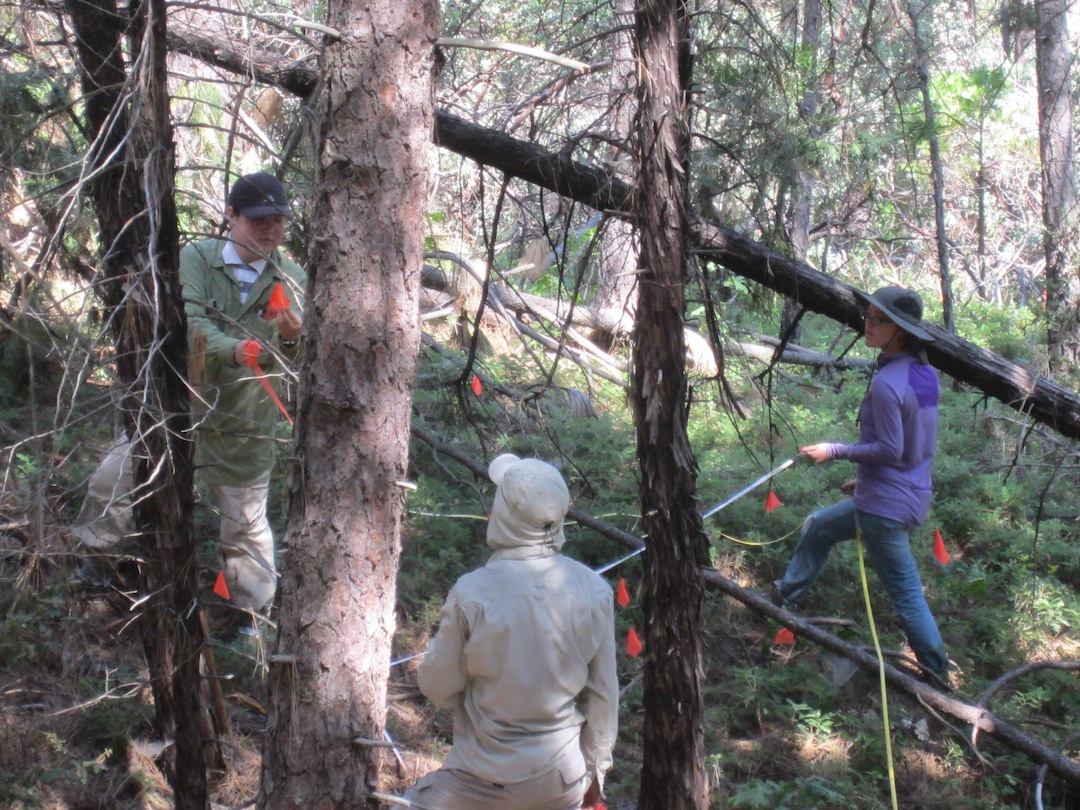
\includegraphics[height=7cm]{./Images/IMG_6525}
\end{figure}
\end{frame}

% --- slide ------------------------------------------------
\begin{frame}{Field Campaigns in Pictures}
\vspace{-.5cm}
\begin{figure}
\centering
    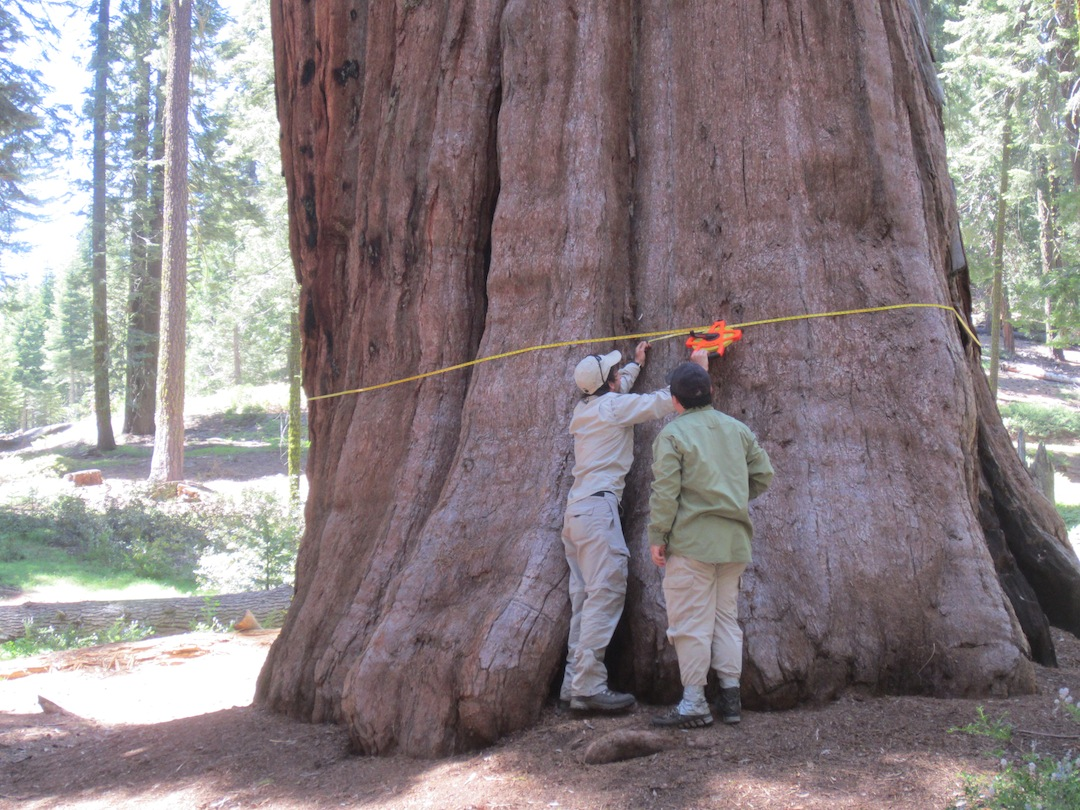
\includegraphics[height=7cm]{./Images/IMG_6637}
\end{figure}
\end{frame}

% --- slide ------------------------------------------------
\begin{frame}{Field Campaigns in Pictures}
\vspace{-.5cm}
\begin{figure}
\centering
    \includegraphics[height=7cm]{./Images/IMG_7811}
\end{figure}
\end{frame}

% --- slide ------------------------------------------------
\begin{frame}{Field Campaigns in Pictures}
\vspace{-.5cm}
\begin{figure}
\centering
    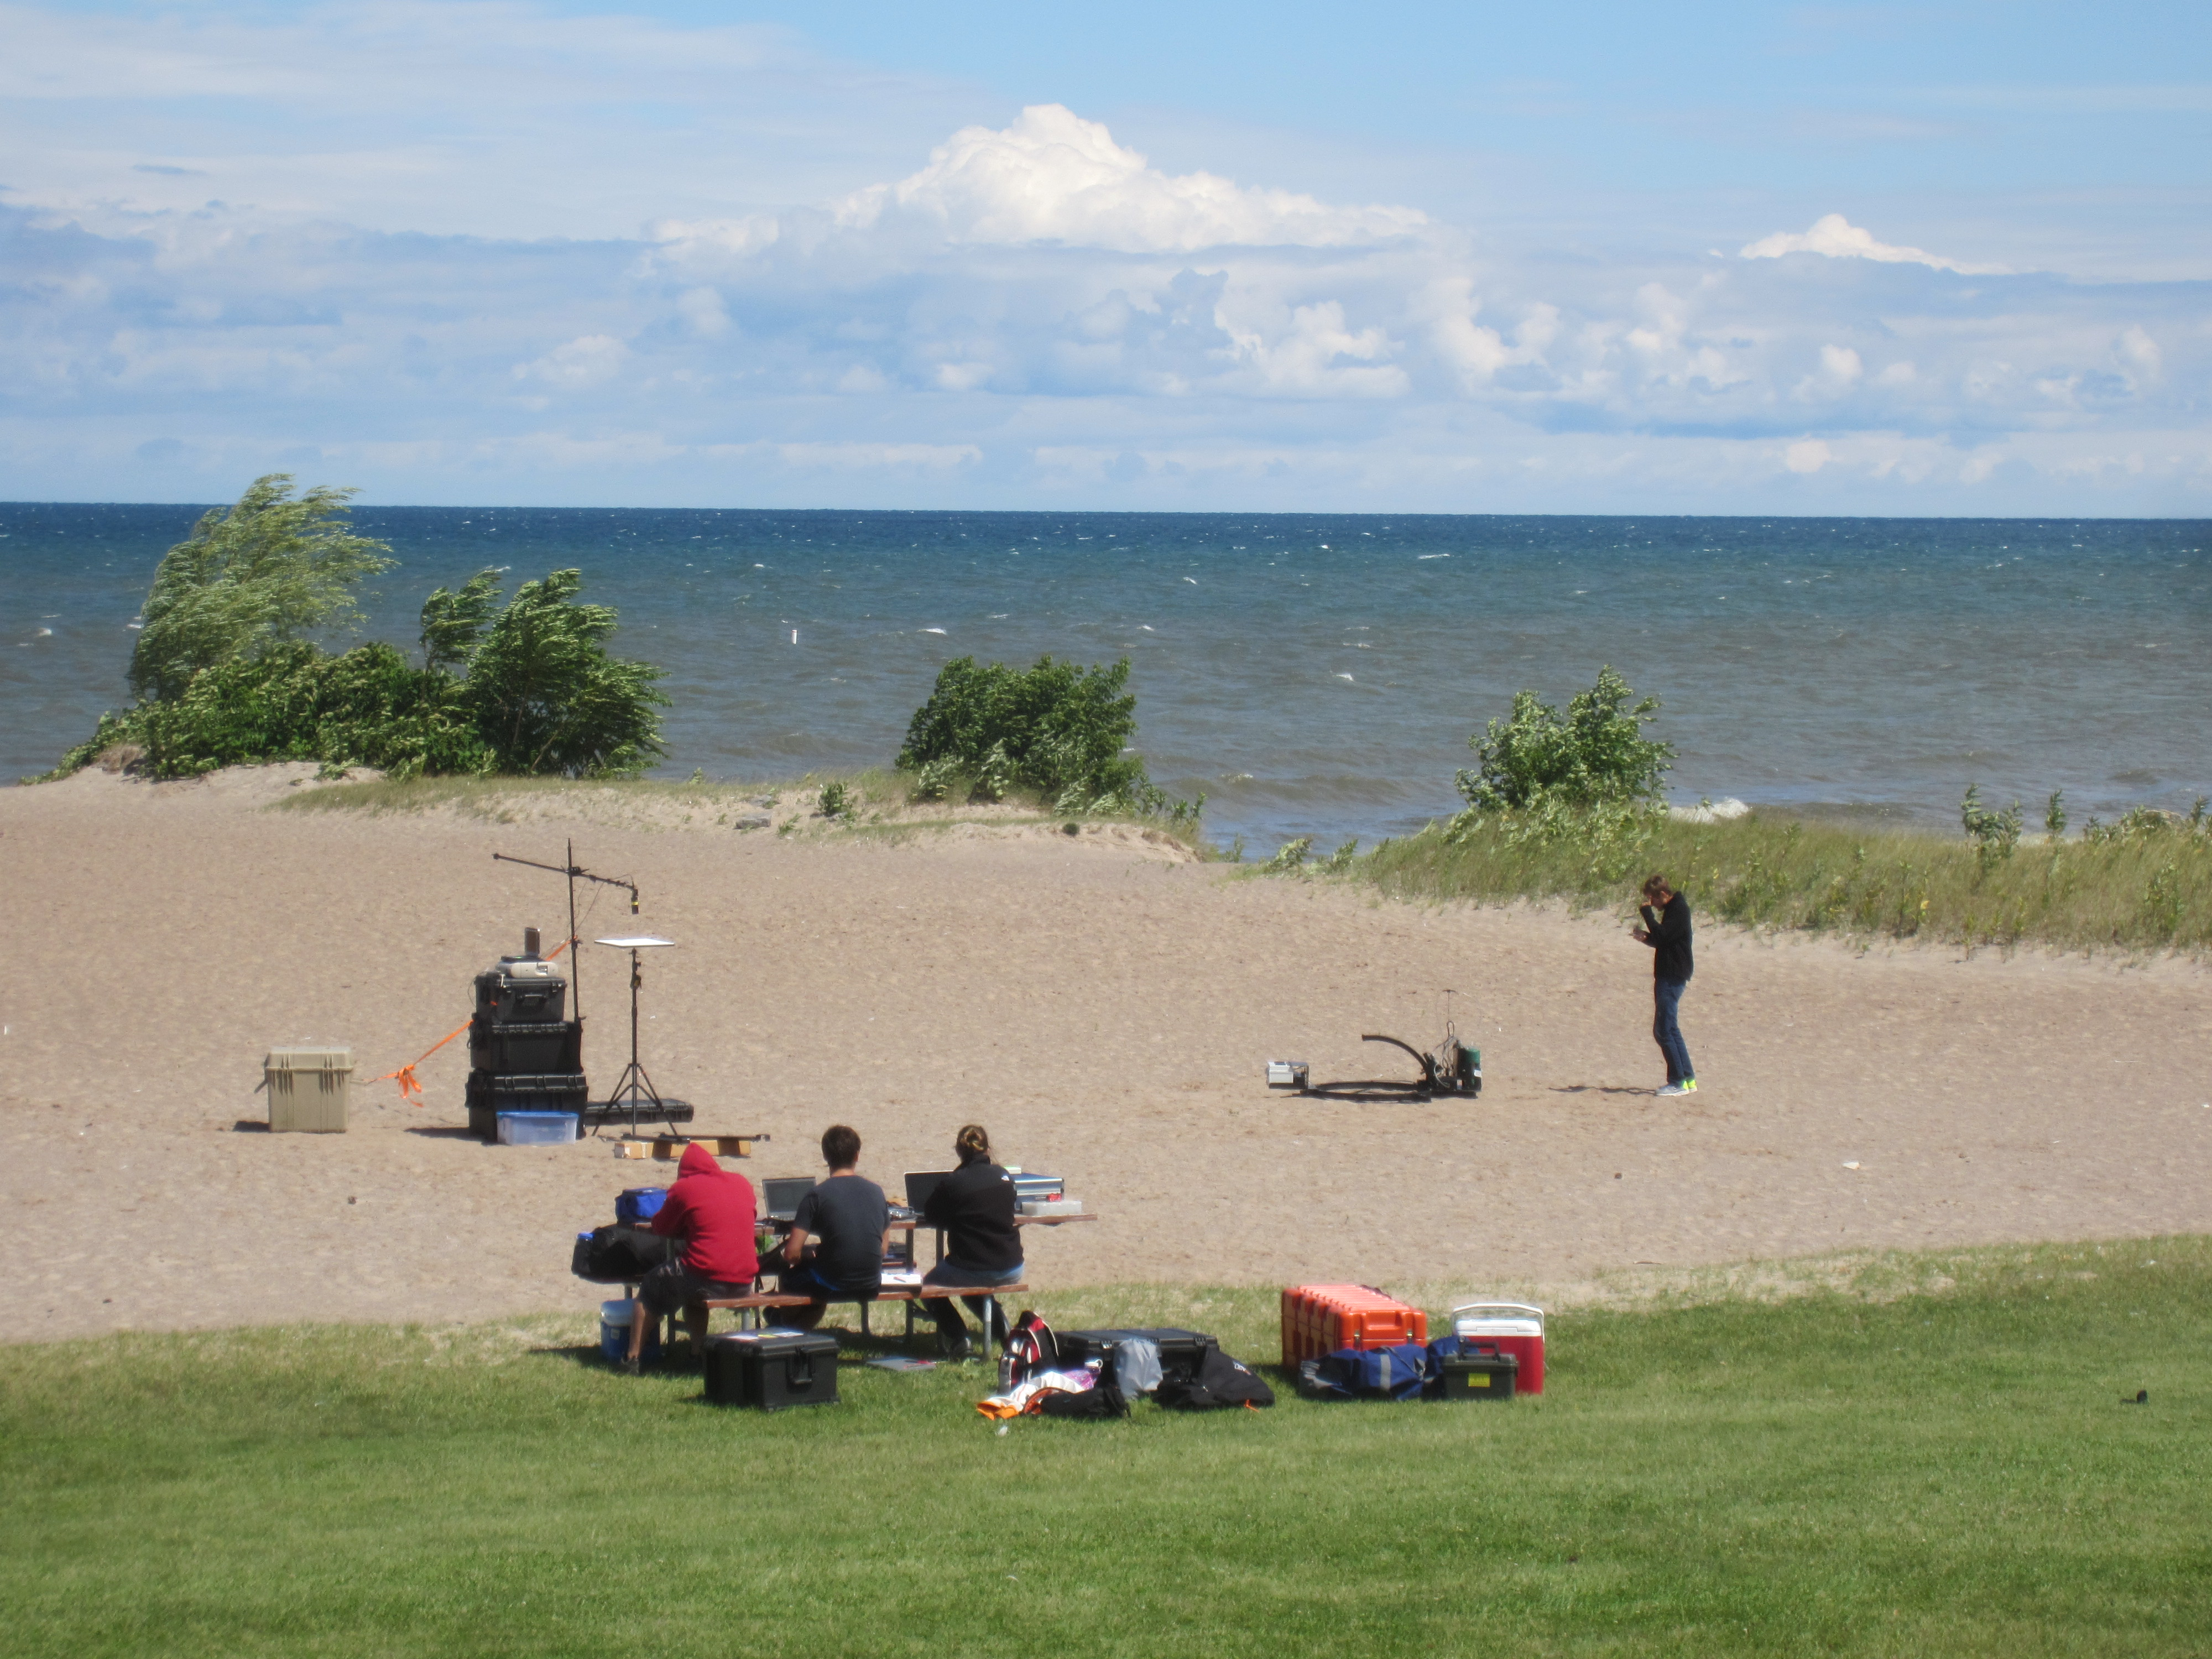
\includegraphics[height=7cm]{./Images/IMG_7932}
\end{figure}
\end{frame}

% --- slide ------------------------------------------------
\begin{frame}{Field Campaigns in Pictures}
\vspace{-.5cm}
\begin{figure}
\centering
    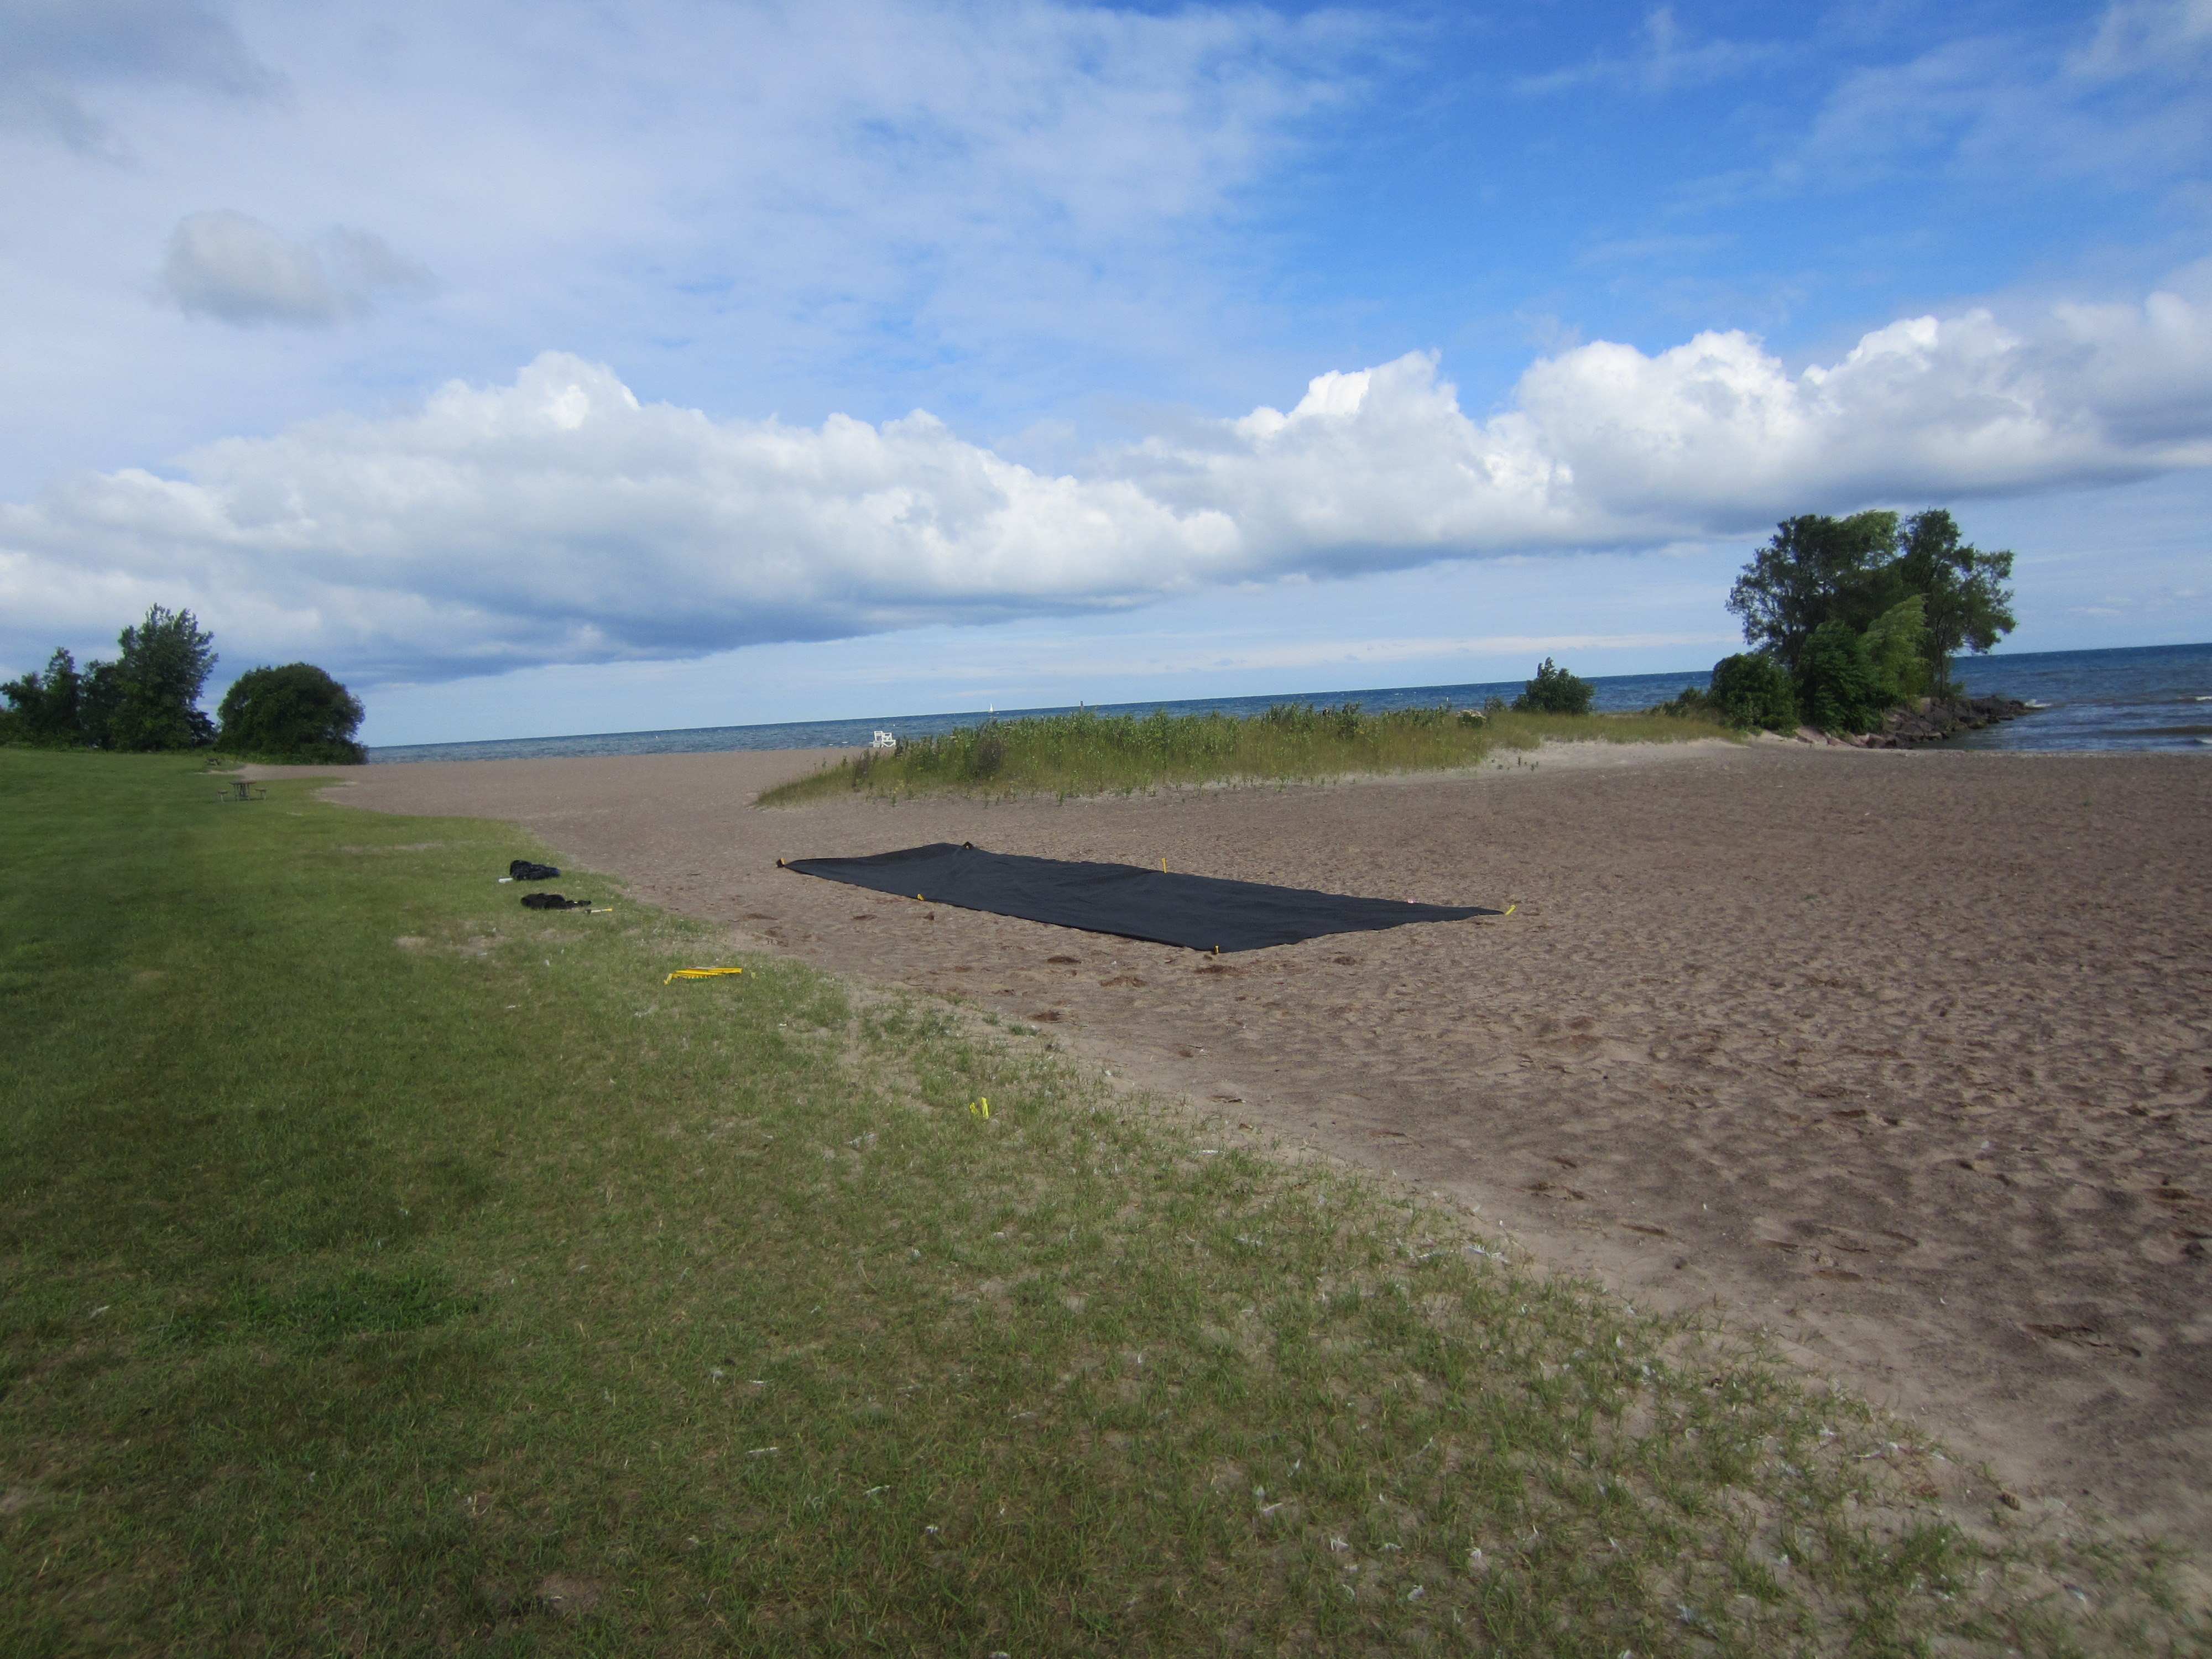
\includegraphics[height=7cm]{./Images/IMG_7966}
\end{figure}
\end{frame}

% --- slide ------------------------------------------------
\begin{frame}{Field Campaigns in Pictures}
\vspace{-.5cm}
\begin{figure}
\centering
    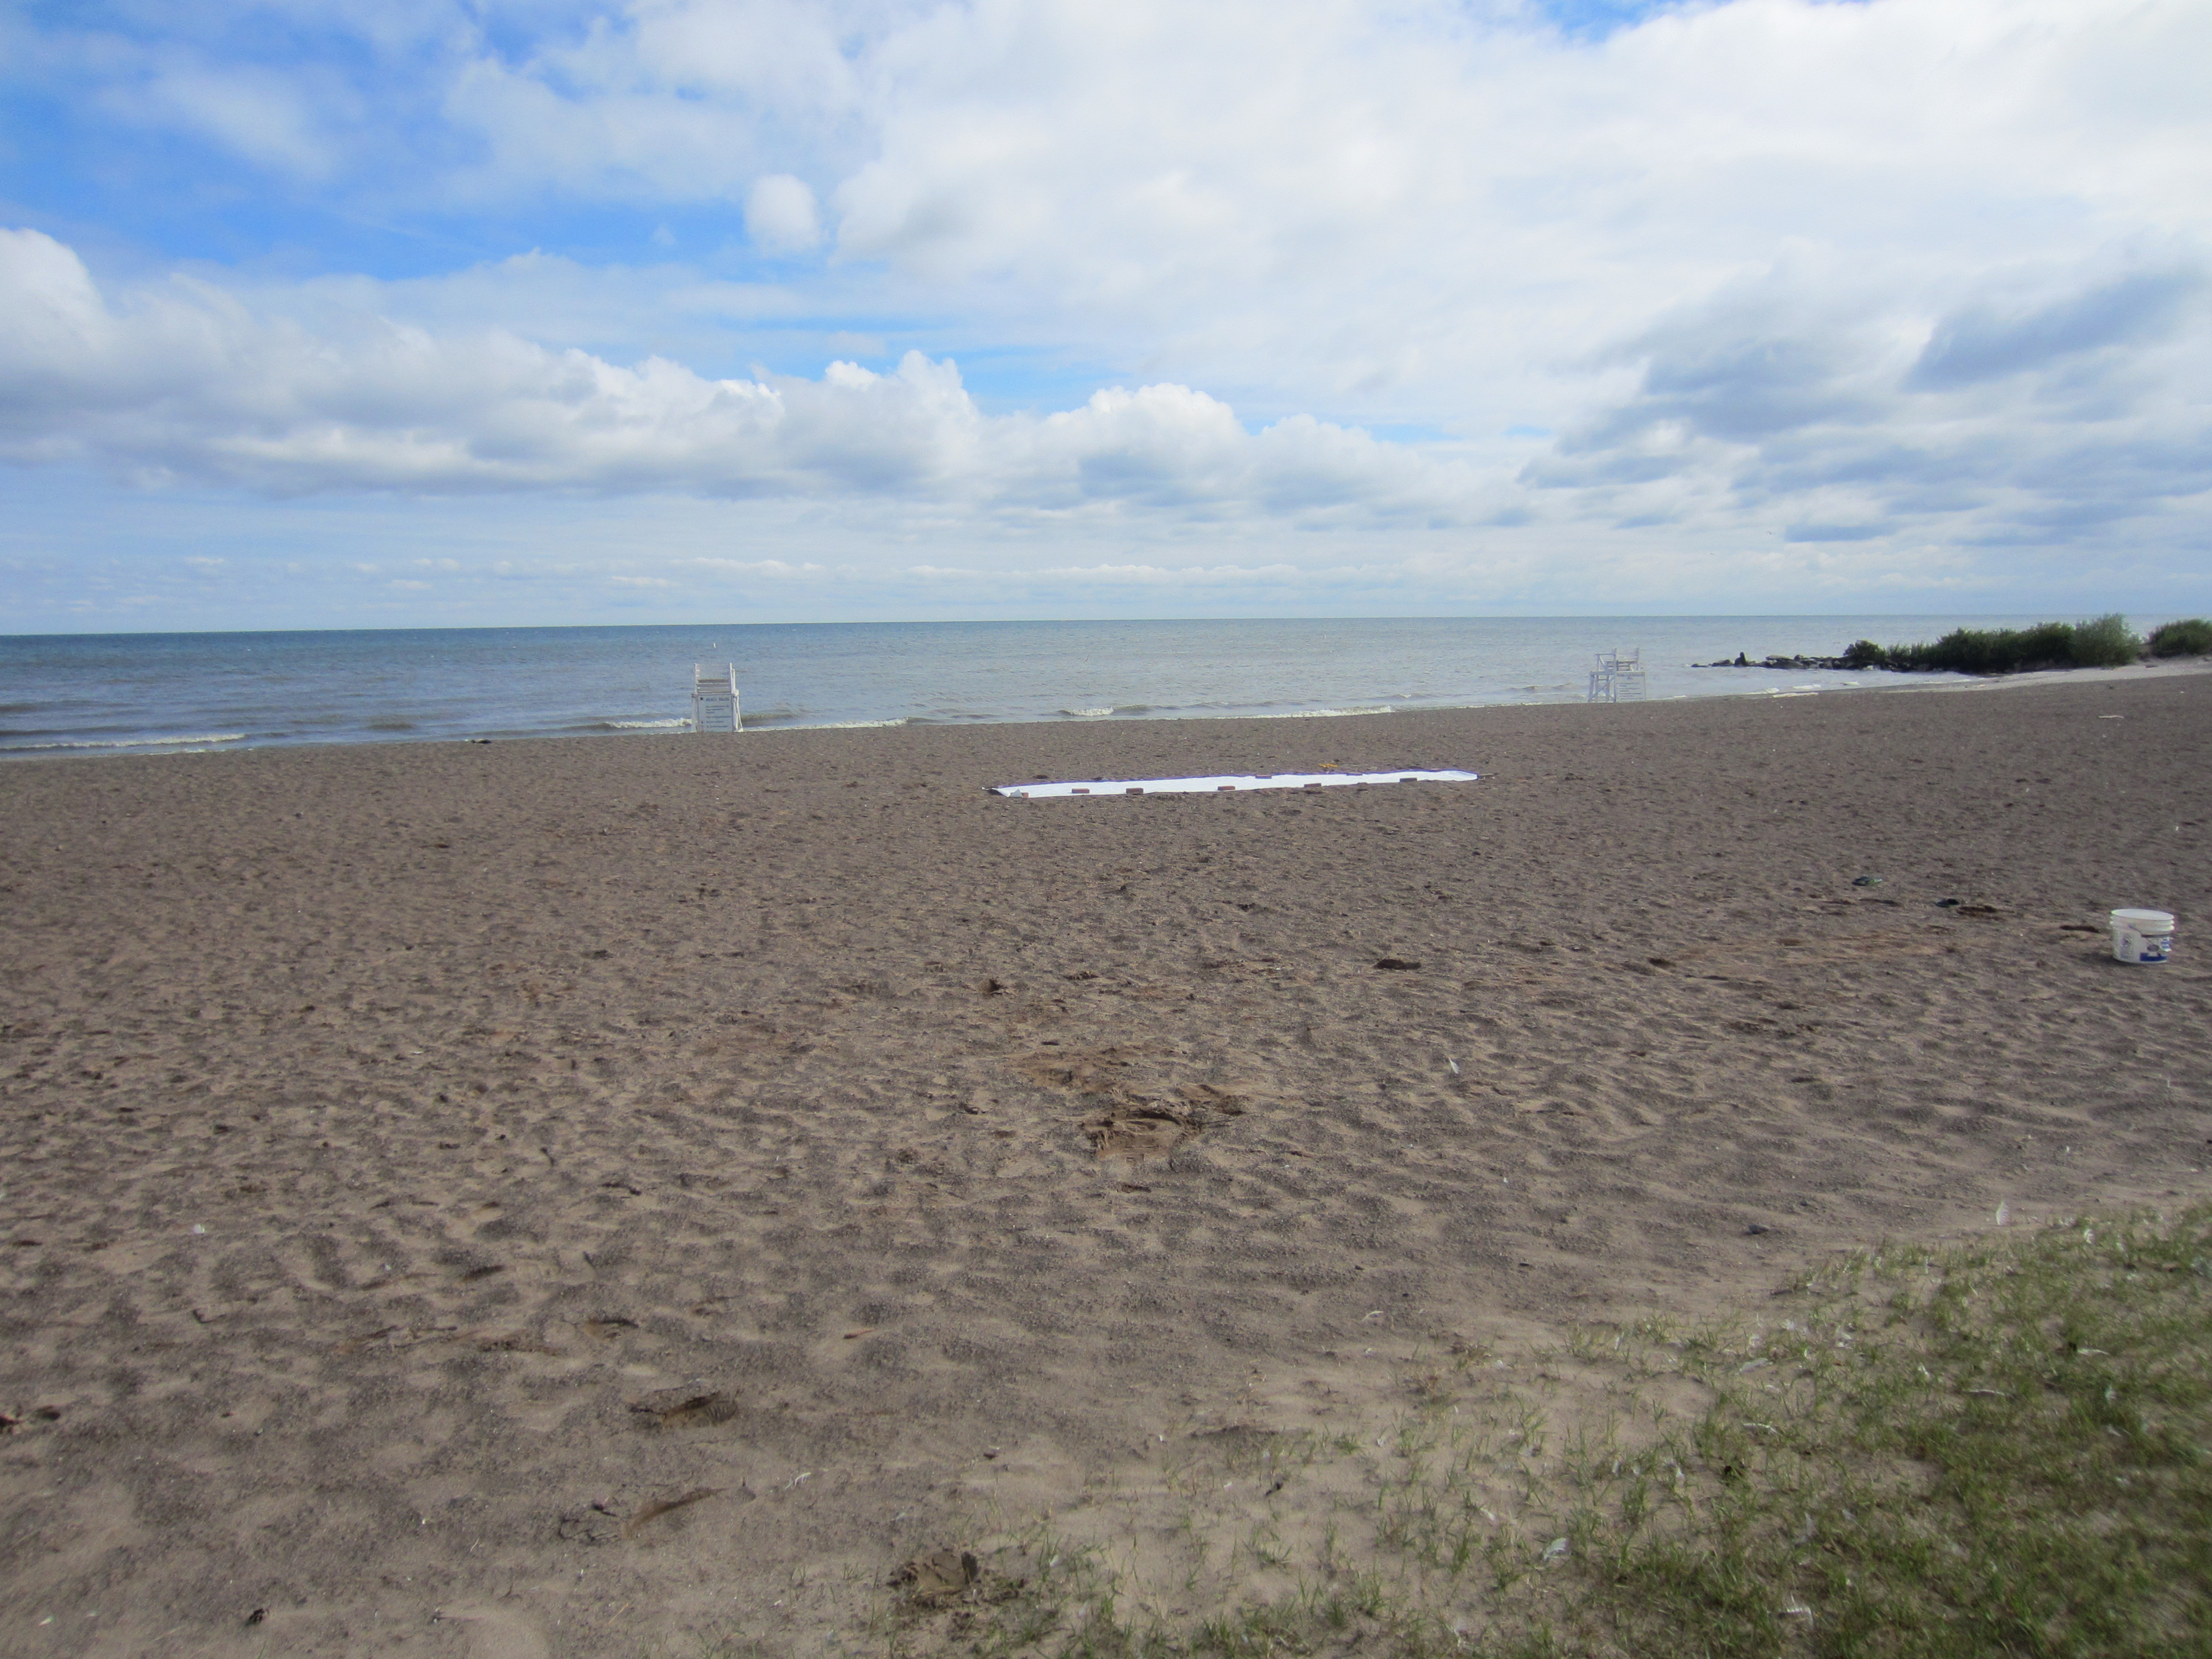
\includegraphics[height=7cm]{./Images/IMG_7967}
\end{figure}
\end{frame}

% --- slide ------------------------------------------------
\begin{frame}{Field Campaigns in Pictures}
\vspace{-.5cm}
\begin{figure}
\centering
    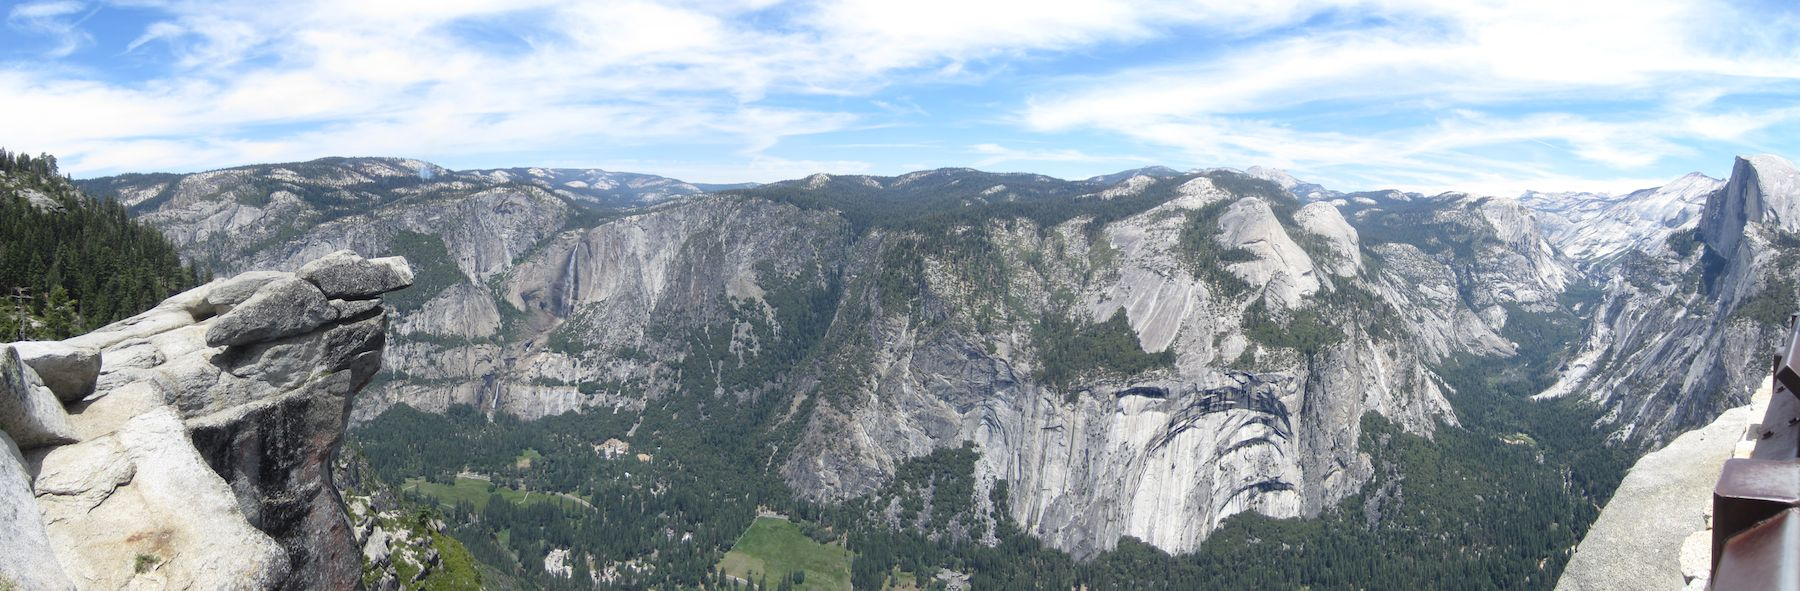
\includegraphics[width=10cm]{./Images/STA_6366-STC_6368}
\end{figure}
\end{frame}




%% Javier

% --- slide ------------------------------------------------
\begin{frame}{Field Campaigns in Pictures}
\vspace{-.5cm}
\begin{figure}
\centering
    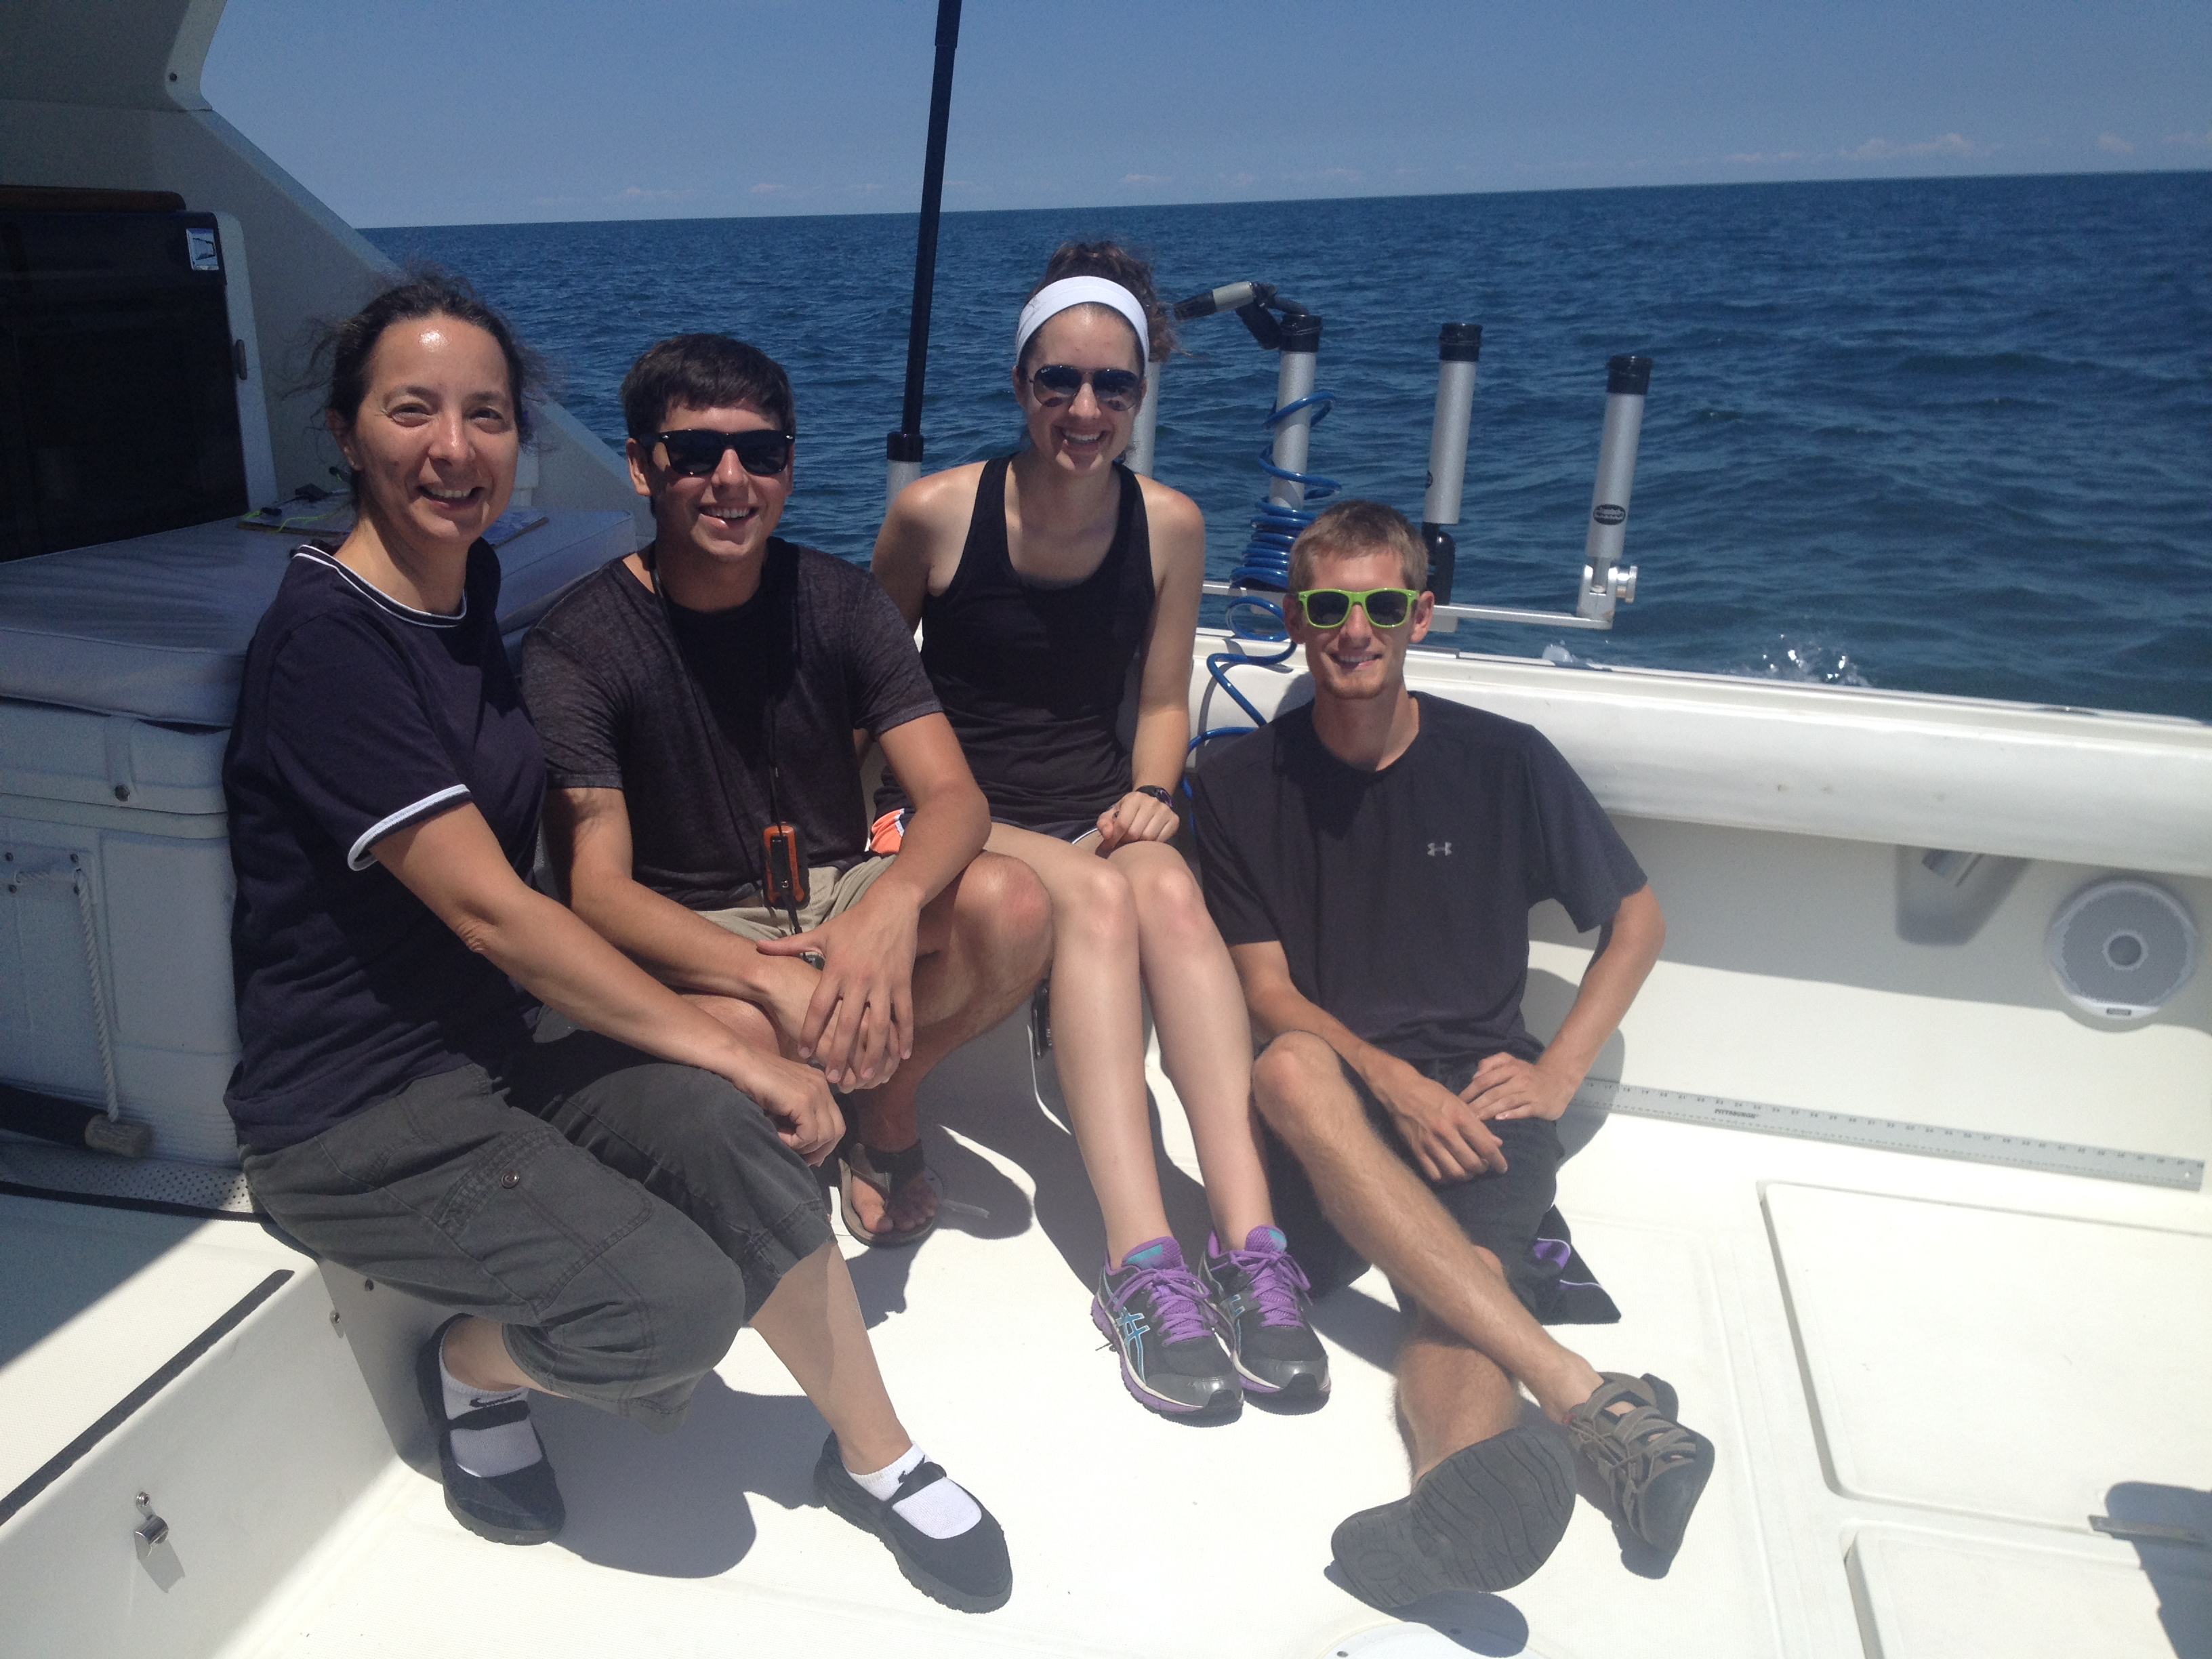
\includegraphics[height=7cm]{./Images/BoatLuxury.jpg}
\end{figure}

\end{frame}
% --- slide ------------------------------------------------
\begin{frame}{Field Campaigns in Pictures}
\vspace{-.5cm}
\begin{figure}
\centering
    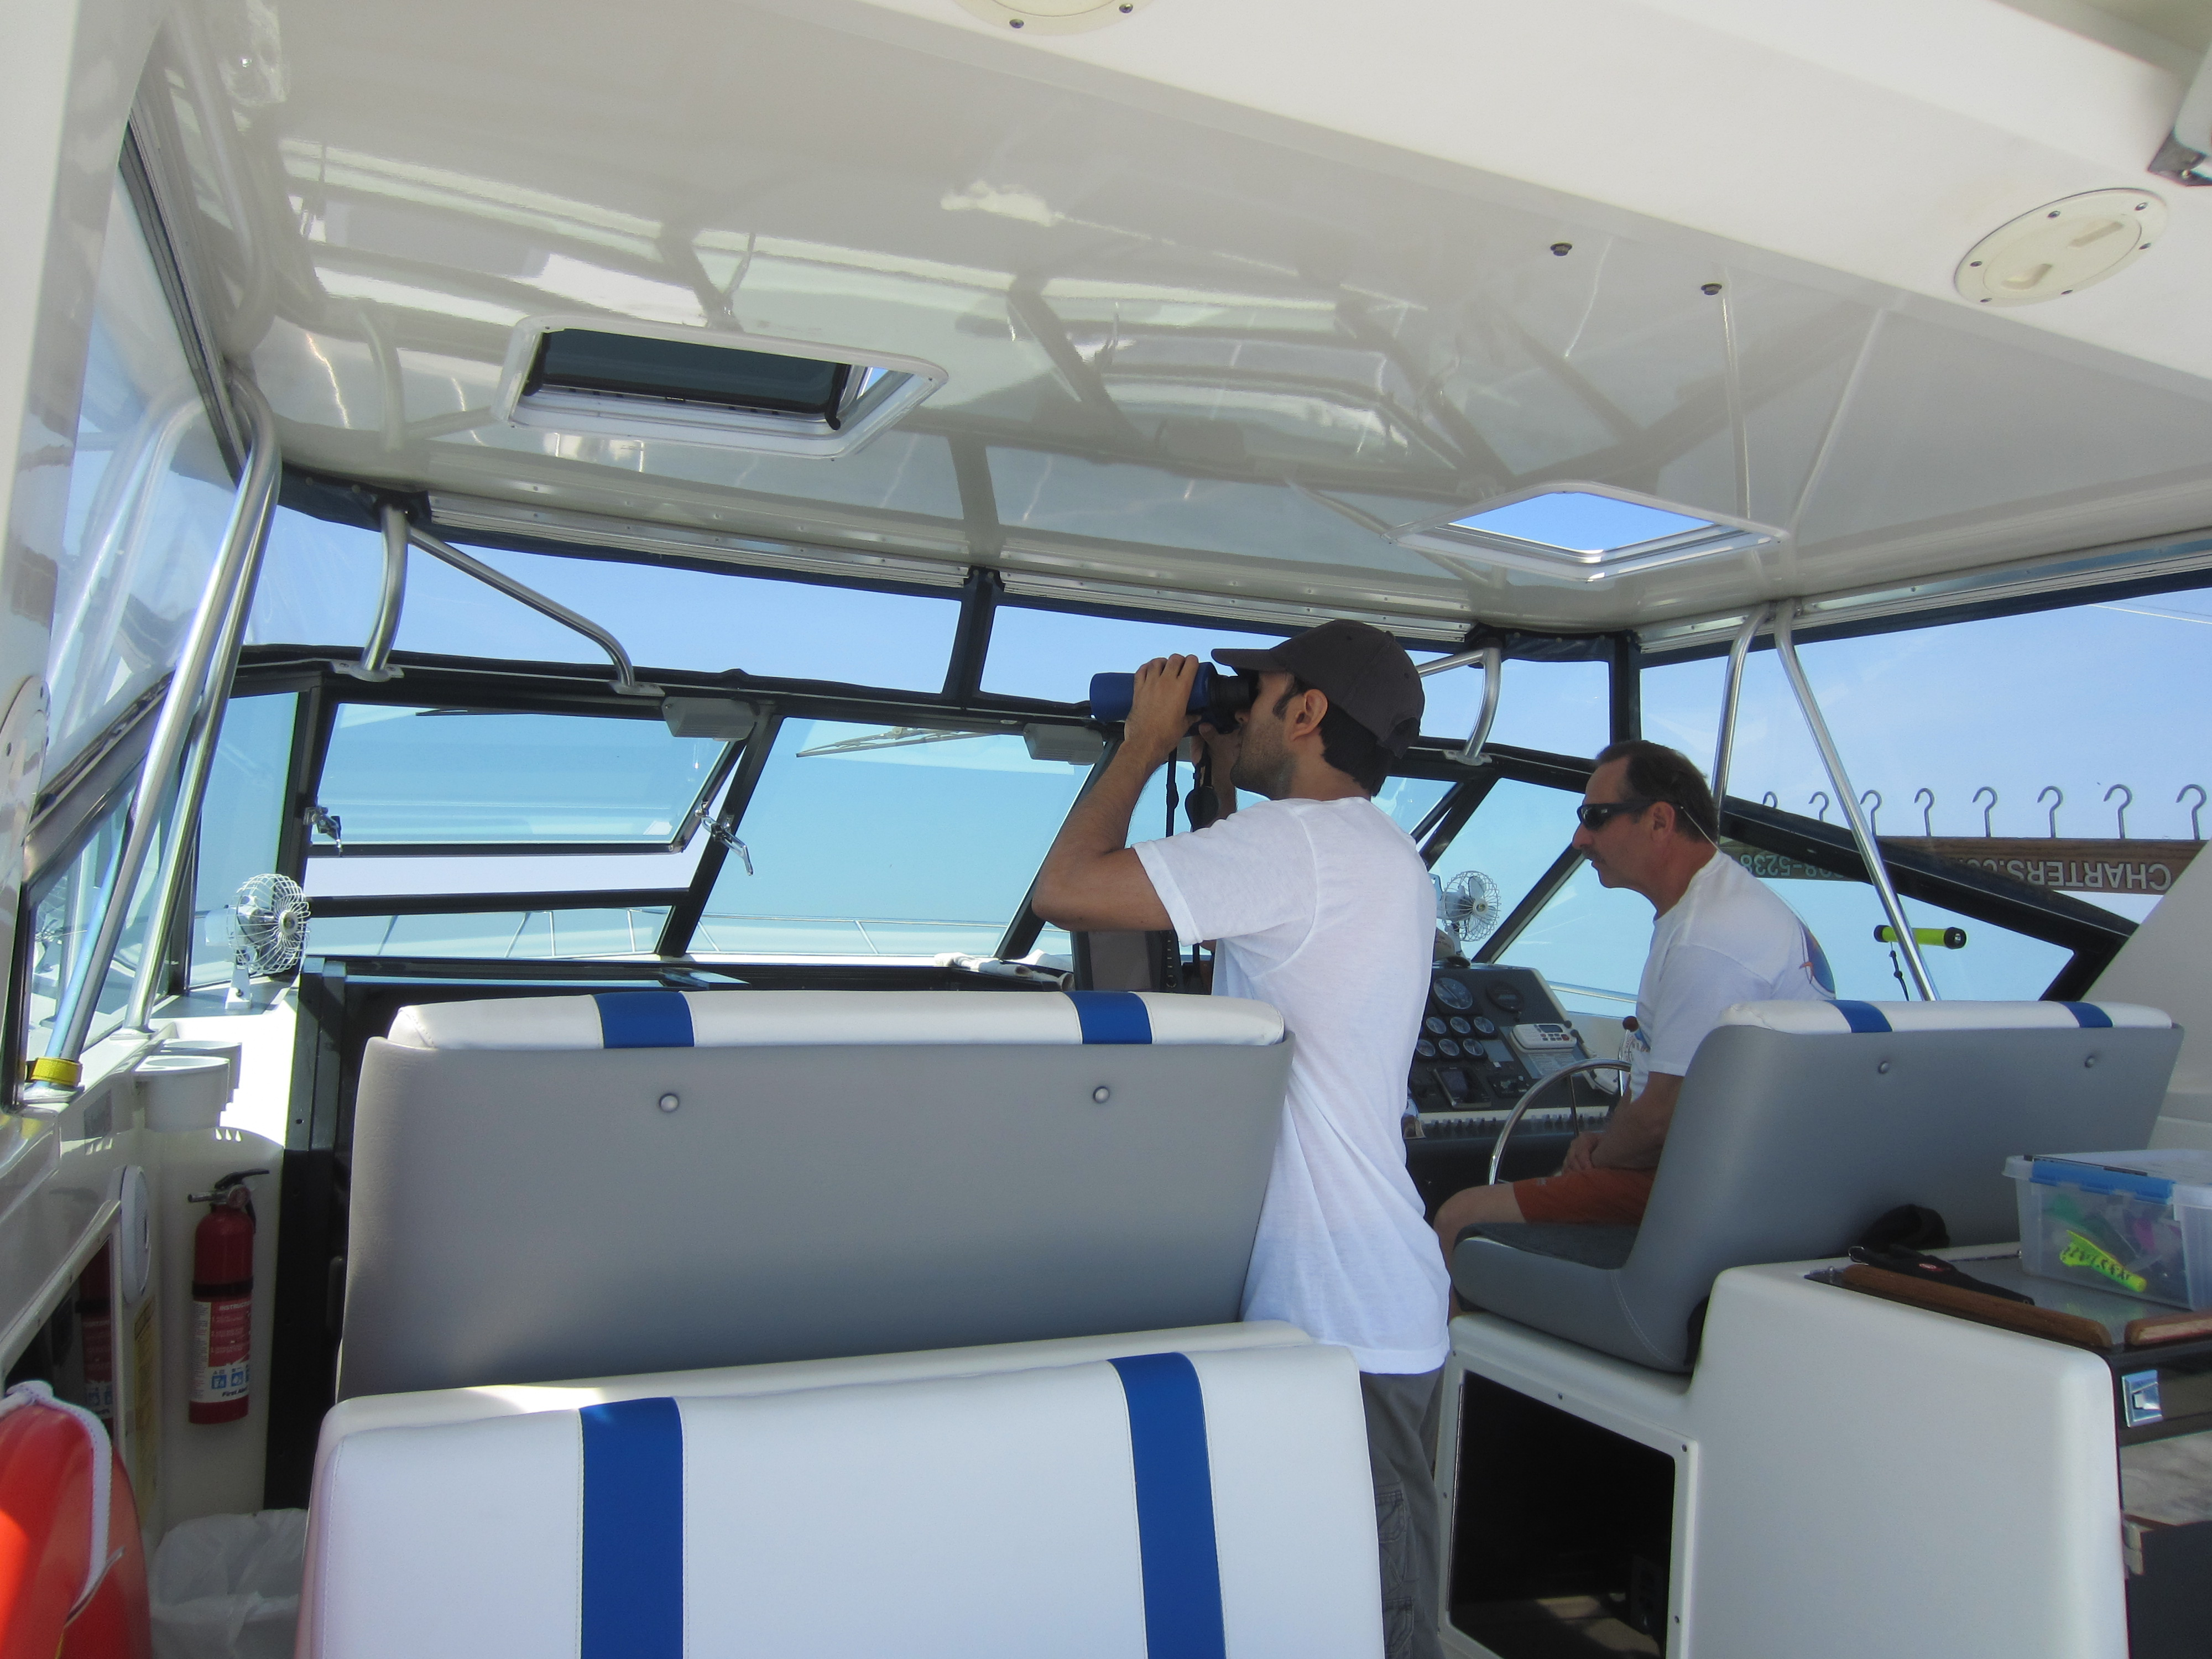
\includegraphics[height=7cm]{./Images/BoatLuxury2.jpg}
\end{figure}

\end{frame}
% --- slide ------------------------------------------------
\begin{frame}{Field Campaigns in Pictures}
\vspace{-.5cm}
\begin{figure}
\centering
    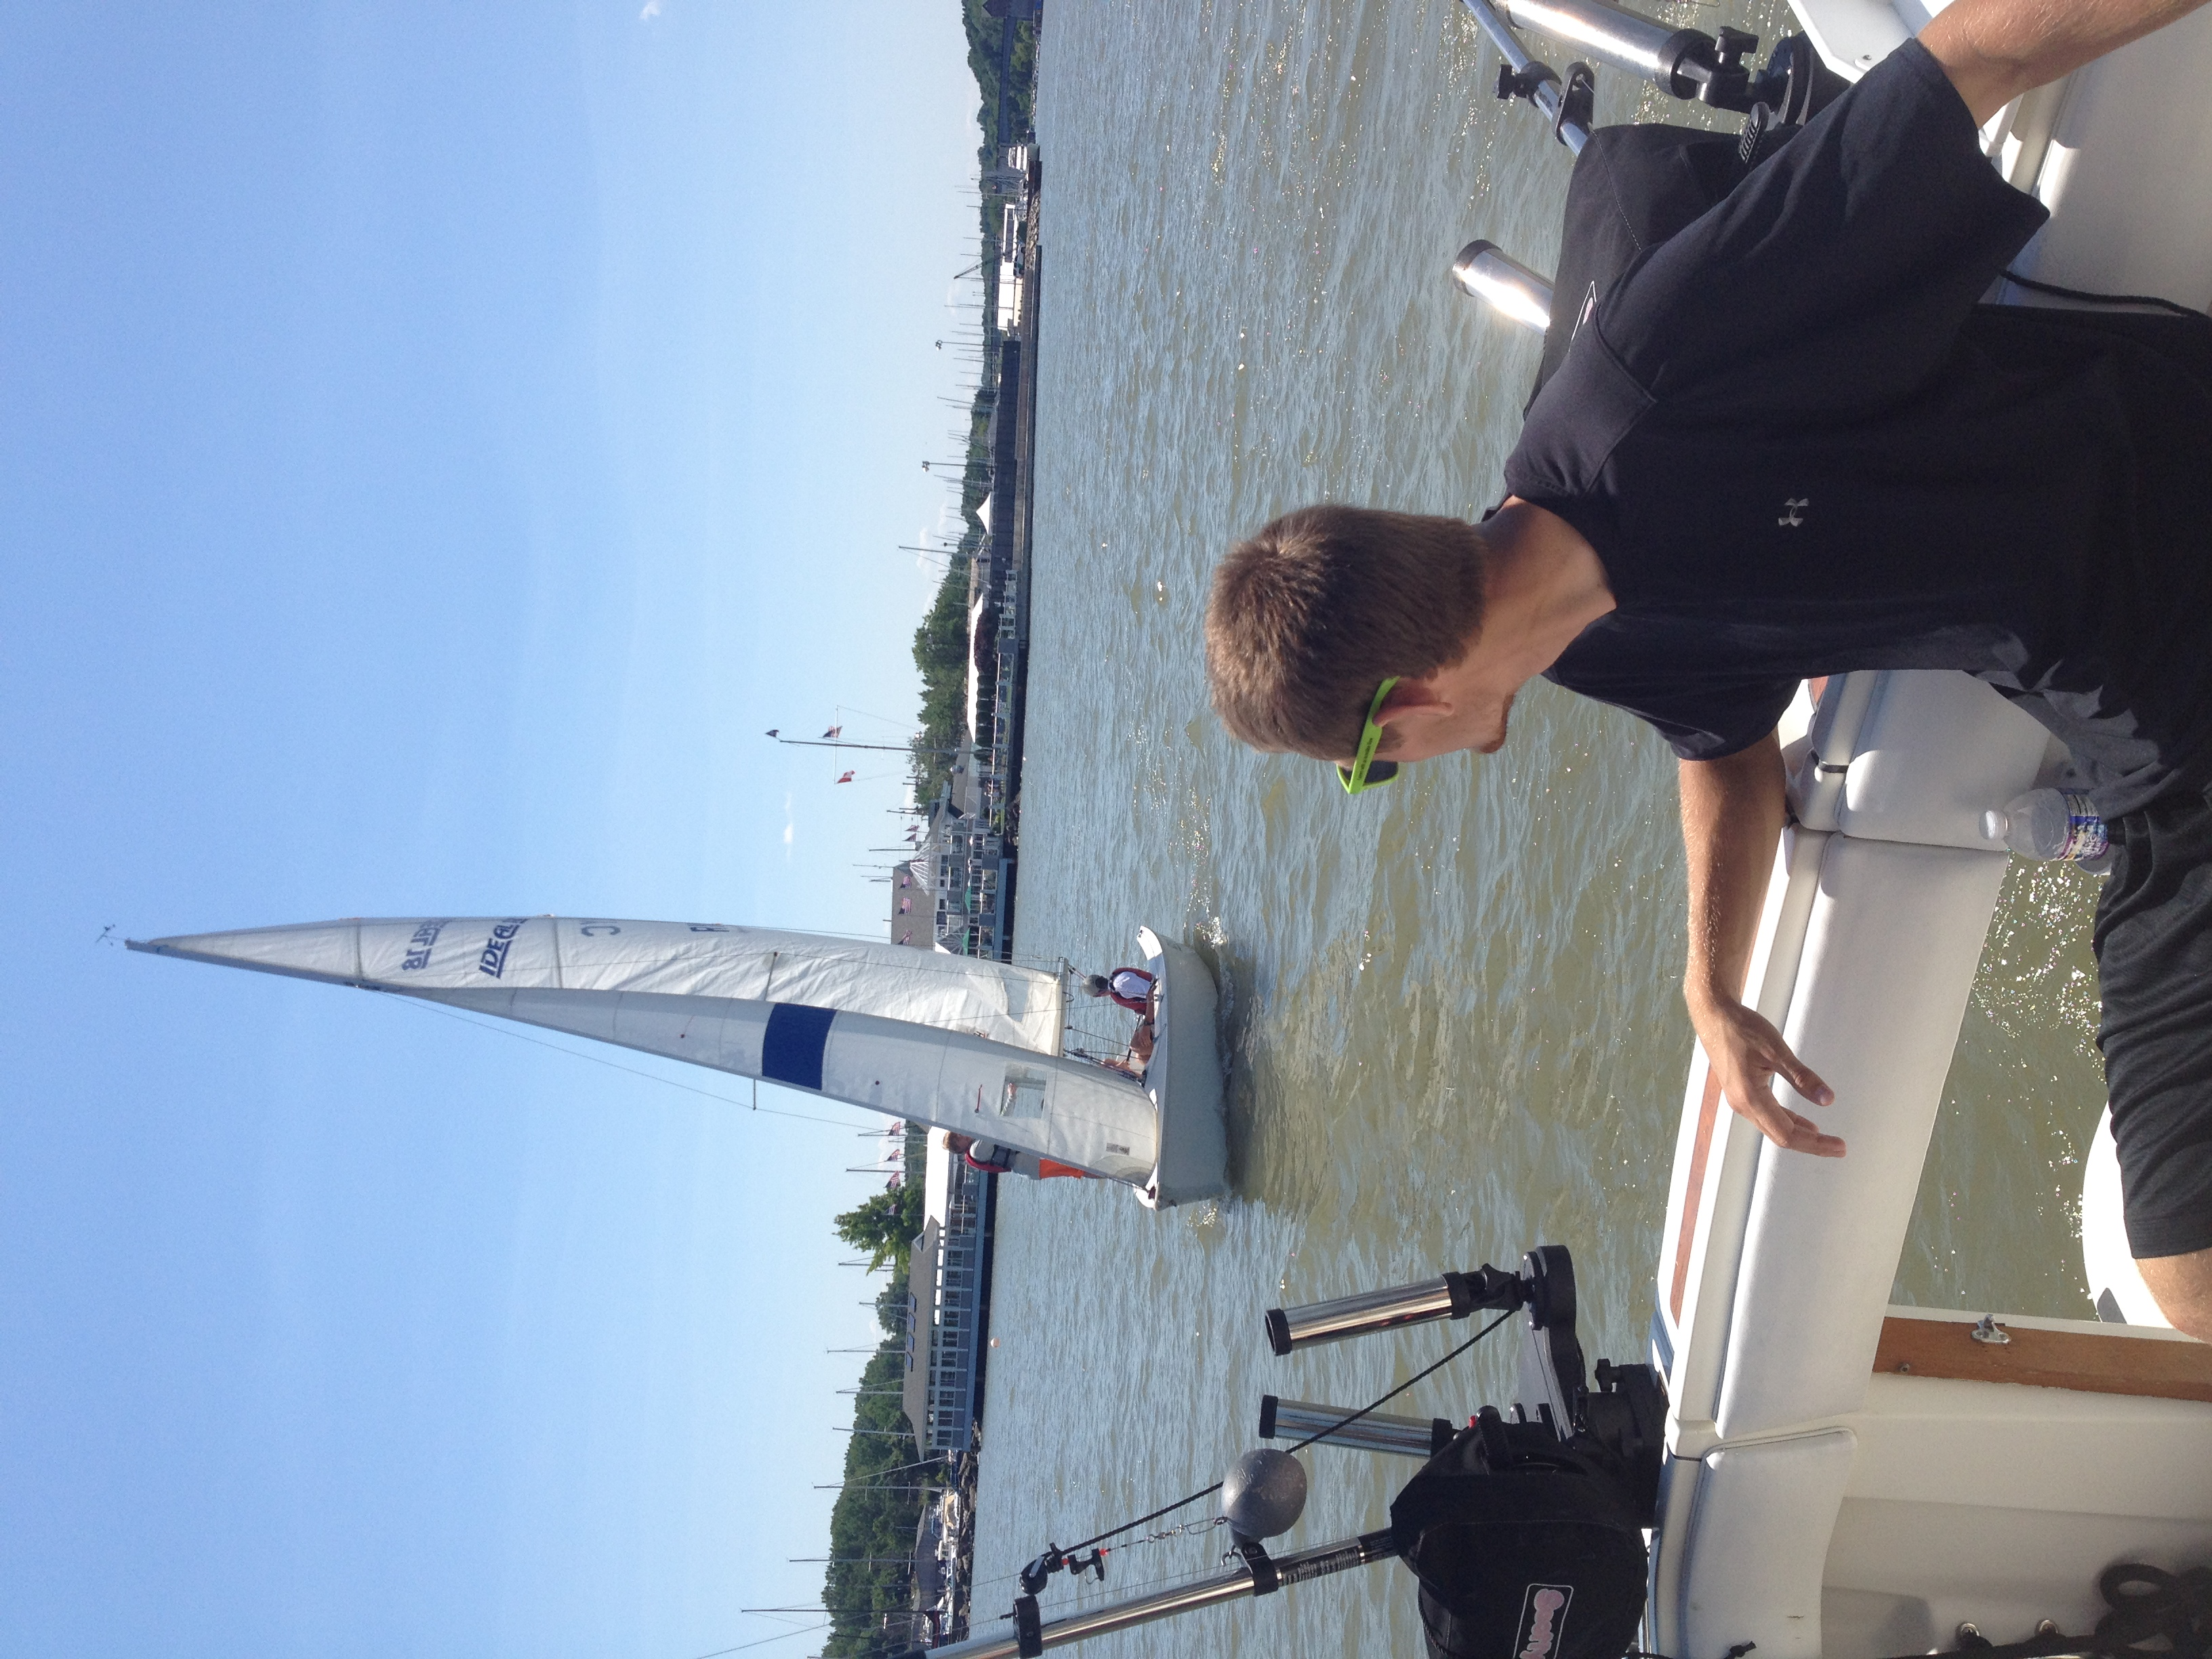
\includegraphics[angle=-90,origin=c,height=6.5cm]{./Images/Boat.jpg}
\end{figure}

\end{frame}
% --- slide ------------------------------------------------
\begin{frame}{Field Campaigns in Pictures}
\vspace{-.5cm}
\begin{figure}
\centering
    \includegraphics[height=7cm]{./Images/SAM_1370.jpg}
\end{figure}

\end{frame}
% --- slide ------------------------------------------------
\begin{frame}{Field Campaigns in Pictures}
\vspace{-.5cm}
\begin{figure}
\centering
    \includegraphics[height=7cm]{./Images/JavierBoat.jpg}
\end{figure}

\end{frame}
% --- slide ------------------------------------------------
\begin{frame}{Field Campaigns in Pictures}
\vspace{-.5cm}
\begin{figure}
\centering
    \includegraphics[angle=90,origin=c,height=6.5cm]{./Images/PaulBoat2.jpg}
\end{figure}

\end{frame}
% --- slide ------------------------------------------------
\begin{frame}{Field Campaigns in Pictures}
\vspace{-.5cm}
\begin{figure}
\centering
    \includegraphics[height=7cm]{./Images/CanoePrep.jpg}
\end{figure}

\end{frame}
% --- slide ------------------------------------------------
\begin{frame}{Field Campaigns in Pictures}
\vspace{-.5cm}
\begin{figure}
\centering
    \includegraphics[angle=-90,origin=c,height=6.5cm]{./Images/CanoeTransport.jpg}
\end{figure}

\end{frame}
% --- slide ------------------------------------------------
\begin{frame}{Field Campaigns in Pictures}
\vspace{-.5cm}
\begin{figure}
\centering
    \includegraphics[height=7cm]{./Images/CanoePrep2.jpg}
\end{figure}

\end{frame}
% --- slide ------------------------------------------------
\begin{frame}{Field Campaigns in Pictures}
\vspace{-.5cm}
\begin{figure}
\centering
    \includegraphics[height=7cm]{./Images/CanoeOnWater.jpg}
\end{figure}

\end{frame}
% --- slide ------------------------------------------------
\begin{frame}{Field Campaigns in Pictures}
\vspace{-.5cm}
\begin{figure}
\centering
    \includegraphics[height=7cm]{./Images/JavierPaddle.jpg}
\end{figure}

\end{frame}
% --- slide ------------------------------------------------
\begin{frame}{Field Campaigns in Pictures}
\vspace{-.5cm}
\begin{figure}
\centering
    \includegraphics[angle=90,origin=c,height=6.5cm]{./Images/JavierCanoe.jpg}
\end{figure}

\end{frame}
% --- slide ------------------------------------------------
\begin{frame}{Field Campaigns in Pictures}
\vspace{-.5cm}
\begin{figure}
\centering
    \includegraphics[height=7cm]{./Images/NastyWater.jpg}
\end{figure}

\end{frame}
% --- slide ------------------------------------------------
\begin{frame}{Field Campaigns in Pictures}
\vspace{-.5cm}
\begin{figure}
\centering
    \includegraphics[height=7cm]{./Images/PaulCanoe.jpg}
\end{figure}

\end{frame}
% --- slide ------------------------------------------------
\begin{frame}{Field Campaigns in Pictures}
\vspace{-.5cm}
\begin{figure}
\centering
    \includegraphics[height=7cm]{./Images/PaulCanoeFeet.jpg}
\end{figure}

\end{frame}
% --- slide ------------------------------------------------
\begin{frame}{Field Campaigns in Pictures}
\vspace{-.5cm}
\begin{figure}
\centering
    \includegraphics[height=7cm]{./Images/PaulSand.jpg}
\end{figure}

\end{frame}
% --- slide ------------------------------------------------
\begin{frame}{Field Campaigns in Pictures}
\vspace{-.5cm}
\begin{figure}
\centering
    \includegraphics[height=7cm]{./Images/Birds2.jpg}
\end{figure}

\end{frame}
% --- slide ------------------------------------------------
\begin{frame}{Field Campaigns in Pictures}
\vspace{-.5cm}
\begin{figure}
\centering
    \includegraphics[height=7cm]{./Images/Birds.jpg}
\end{figure}



\end{frame}
%%%%%%%%%%%%%%%%%%% SECTION %%%%%%%%%%%%%%%%%%%%%%%%%%%%%%%%
% \section{Conclusions}
% \subsection*{Conclusions}
% % --- slide ------------------------------------------------
% \begin{frame}{\LARGE Conclusions}

% \Large
% \begin{itemize}\itemsep.4cm
% 	\item Current retrieval algorithm depends on IOPs from the field. Not always available!

% 	\item LUT from Hydrolight: Highly dependent in phase function

% 	\item Obtain field data for Landsat-8 is difficult, mainly for weather conditions
% \end{itemize}

% \end{frame}

% --- slide ------------------------------------------------
{	
\setbeamertemplate{footline}{} 
\setbeamertemplate{headline}{}
\begin{frame}[noframenumbering] 

\vspace{\baselineskip}
\centerline{\Large Thanks for your attention!}
	\vspace{\baselineskip}
\vspace{-.3cm}
% \centerline{\Huge QUESTIONS?}
\uncover <2->{\centerline{\Huge QUESTIONS?}}

\begin{figure}[htb]
\centering
\includegraphics[height=6.5cm]{./Images/NiceView.jpg}
\end{figure}
\end{frame}
}
% % BIBLIOGRAPHY
% \bibliographystyle{apalike}

% \bibliography{/Users/javier/Desktop/Javier/PHD_RIT/Latex/javier_bib}
% --- slide ------------------------------------------------
\section*{}
\begin{frame}%[shrink=30] 
\tiny
  \frametitle{References}
  % \nocite{*}
  \bibliographystyle{apalike}
  \bibliography{./javier_bib}
\end{frame}
\end{document} 
% EEEEEEEEEEENNNNNNNNNNNNNNDDDDDDDDDDDD